
\documentclass[12pt, twoside]{book}
%%%%%%%% Preamble %%%%%%%%%%%%
\title{Degree project}
\usepackage[utf8]{inputenc} % File coding uses utf8
\usepackage{amsmath} % Extra commands for math
\usepackage{amssymb} % Math symbols 
\usepackage{graphicx} % Include images in LaTeX
\usepackage{color} % Coloring text
\usepackage{enumerate}
\usepackage{titletoc}
\usepackage{float} % Allow you to use [H] specifier to force the position of the images 
\usepackage{capt-of} % Defines a command \captionof for putting a caption to something that’s not a float.
\usepackage{sidecap} % Defines environments called SCfigure and SCtable (analogous to figure and table) to typeset captions sideways
\sidecaptionvpos{figure}{c} % Alignment
\usepackage{caption} % to customize the captions in floating environments like figure and table
\usepackage{commath} % Mathematics typesetting support
\usepackage{cancel} % Place lines through maths formulae
\usepackage{anysize} % to set up document margins
\marginsize{3.5cm}{2cm}{2.54cm}{2.54cm} % Left, right, up, down
\usepackage{wrapfig}
% \usepackage[top=2.54cm,bottom=2.54cm,left=3.5cm,right=2cm]{geometry}
\usepackage{appendix} %Extra control of appendices
\usepackage{tocbibind}
\usepackage{colortbl}

%EXTRA PACKAGES
\usepackage{indentfirst}
\usepackage{multirow}
\usepackage[toc, acronym]{glossaries}
\usepackage[linesnumbered,ruled,vlined]{algorithm2e}
\usepackage{multirow}
\usepackage{tabulary}
\usepackage{enumitem}
\usepackage{enumerate}
\usepackage{changepage}
\usepackage{alltt}
\usepackage{listings}
\usepackage{longtable,lscape}
\usepackage{lmodern}
\usepackage{gensymb}
\usepackage{caption}
\usepackage{subcaption}
\usepackage{hyperref}
\hypersetup{
    colorlinks,
    citecolor=blue,
    filecolor=black,
    linkcolor=black,
    urlcolor=black
}
\usepackage{listings}
\usepackage{color}
\lstloadlanguages{C,C++,csh,Java}

\definecolor{red}{rgb}{0.6,0,0} 
\definecolor{blue}{rgb}{0,0,0.6}
\definecolor{green}{rgb}{0,0.8,0}
\definecolor{cyan}{rgb}{0.0,0.6,0.6}
\definecolor{gray}{rgb}{0.753,0.753,0.753}

\lstset{
language=csh,
basicstyle=\footnotesize\ttfamily,
numbers=left,
numberstyle=\tiny,
numbersep=5pt,
tabsize=2,
extendedchars=true,
breaklines=true,
frame=b,
stringstyle=\color{blue}\ttfamily,
showspaces=false,
showtabs=false,
commentstyle=\color{green},
morecomment=[l]{//}, %use comment-line-style!
morecomment=[s]{/*}{*/}, %for multiline comments
showstringspaces=false,
morekeywords={ abstract, event, new, struct,
as, explicit, null, switch,
base, extern, object, this,
bool, false, operator, throw,
break, finally, out, true,
byte, fixed, override, try,
case, float, params, typeof,
catch, for, private, uint,
char, foreach, protected, ulong,
checked, goto, public, unchecked,
class, if, readonly, unsafe,
const, implicit, ref, ushort,
continue, in, return, using,
decimal, int, sbyte, virtual,
default, interface, sealed, volatile,
delegate, internal, short, void,
do, is, sizeof, while,
double, lock, stackalloc,
else, long, static,
enum, namespace, string},
keywordstyle=\color{cyan},
identifierstyle=\color{red},
backgroundcolor=\color{white},
}

\usepackage{caption}
\DeclareCaptionFont{white}{\color{white}}
\DeclareCaptionFormat{listing}{\colorbox{blue}{\parbox{\textwidth}{\hspace{15pt}#1#2#3}}}
\captionsetup[lstlisting]{format=listing,labelfont=white,textfont=white, singlelinecheck=false, margin=0pt, font={bf,footnotesize}}

\lstdefinestyle{sharpc}{language=[Sharp]C, frame=lr, rulecolor=\color{blue!80!black}}

% Reset page margins properly for doublesided pages
\setlength{\marginparwidth}{0pt}
\setlength{\marginparsep}{0pt}
\setlength{\oddsidemargin}{0.125in}
\setlength{\evensidemargin}{0.125in}
\setlength{\textwidth}{6.375in}
\setlength{\parindent}{1em}
\setlength{\tabcolsep}{18pt}
\raggedbottom


%%% Theorem-like environments %%%%%%%%%%%%%%%%%%%%%%%%%%%%%%%%%%%%%%%%%%%%%%%%%%
%%\usepackage{mathtools}

\newtheorem{theorem}{Theorem}
\newtheorem{corollary}{Corollary}
\newtheorem{lemma}{Lemma}
\newtheorem{proposition}{Proposition}
\newtheorem{conjecture}{Conjecture}
\newtheorem{definition}{Definition}
\newtheorem{remark}{Remark}
\newtheorem{example}{Example}

%%%%%%%%%%%%%%%%%%%%%%%%%%%%%%%%%%%%%%%%%%%%%%%%%%%%%%%%%%%%%%%%%%%%%%%%%%%%%%%%

%%% Put your local definitions here %%%%%%%%%%%%%%%%%%%%%%%%%%%%%%%%%%%%%%%%%%%%
% For example,
\newcommand{\R}{\mathbb{R}}
\let\cleardoublepage\clearpage

% Header and Footer
\usepackage{fancyhdr} 
\pagestyle{fancy}
\fancyhf{}
\fancyhead[L]{\footnotesize University of Science and Technology of Hanoi} 
\fancyfoot[R]{\footnotesize Bachelor Thesis}  
\fancyfoot[C]{\thepage}  % center
\fancyfoot[L]{\footnotesize Information and Communications Technology}  %left
\renewcommand{\footrulewidth}{0.4pt}
\fancypagestyle{firststyle}
{
   \fancyhf{}
}

\usepackage{listings} % To use source code
\definecolor{dkgreen}{rgb}{0,0.6,0} % Color for using code
% Language to use

%%%%%%%% glossaries %%%%%%%%%%%%
\makeglossaries
\newacronym{usth}{USTH}{University of Science and Technology of Hanoi}

\newacronym{vast}{VAST}{Vietnam Academy of Science and Technology}
\newacronym{api}{API}{application programming interface}
\newacronym{db}{DB}{database}
\newacronym{dbms}{DBMS}{database managment system}
\newacronym{http}{HTTP}{Hypertext Transfer Protocol}

\newacronym{sql}{SQL}{structured query language}

\newacronym{jdbc}{JDBC}{Java Database Connectivity}

\newacronym{json}{JSON}{JavaScript Object Notation}
\newacronym{acl}{ACL}{Access Control List}
\newacronym{rbac}{RBAC}{Role-Based Access Control}

\newglossaryentry{classDiagram}
{
    name=Application package,
    description={A collection of programs or modules that is directed at some generic  application and can be tailored (perhaps with some additions) to the needs of a specific instance of that application.}
}
\newglossaryentry{boundary}
{
    name=Boundary class,
    description={a class that is the boundary of the system and other system or user (which is actor in the use case diagram).}
}
\newglossaryentry{control}
{
    name=Control class,
    description={A control class manages the flow of interaction of the scenario. A control class to achieves use cases in the use case diagram.}
}
\newglossaryentry{entity}
{
    name=Entity class,
    description={An entity is a long-lived, passive class that is responsible for some meaningful 
chunk of information. that class has data.}
}

\newglossaryentry{sequence}
{
    name=Sequence diagram,
    description={an interaction diagram that shows how processes operate with one another and in what order, and shows object interactions arrange in time sequence.}
}

\newglossaryentry{briefDesc}
{
    name=Brief Description,
    description={The models of discourse along with exposition, argumentation and narration about summary, meaning, role of Use Cases.}
}

\newglossaryentry{flow}
{
    name=Flow of Events,
    description={The set of actions ordered to perform a Use Case in the system.}
}

\newglossaryentry{basicFlow}
{
    name=Basic flow,
    description={The set of required actions to perform Use Case in the system.}
}
\newglossaryentry{altFlow}
{
    name=Alternative flow,
    description={Actions that are not compulsory for the Use Case but they are necessary to 
get all provided function of system.}
}

\newglossaryentry{preCon}
{
    name=Pre-Condition,
    description={a statement or set of statements that outline a condition that should be true, 
or conditions that should be true, when the operation is called. The operation is not guaranteed to perform as it should unless the pre-conditions have been met.}
}

\newglossaryentry{postCon}
{
    name=Post-Condition,
    description={a statement or statements describing the condition that will be true when the operation has completed its task. If the operation is correct and the pre-condition(s) met, then the post-condition is guaranteed to be true.}
}

\title{Degree project}

%%%%%%%% Preamble ends %%%%%%%%%%%%

\begin{document}
\linespread{1.25}
%%%%%%%%%%%%%%%%%%%%%%%%%%%%%%%% Cover Page %%%%%%%%%%%%%%%%%%%%%%%%%%%%%%%%%%%%%%%%%%%

\thispagestyle{firststyle}
\begin{center}
  \textsc{\Large University of Science and Technology of Hanoi}
  \vspace*{-3cm}
  \begin{minipage}{0.48\textwidth} 
    \begin{center}
        \includegraphics[scale = 0.2]{images/usth_logo.png}
    \end{center}
  \end{minipage}
  \vspace*{1cm}

  \begin{minipage}{0.9\textwidth} 
    \begin{center}
      \textsc{\LARGE Bachelor Thesis}
    \end{center}
  \end{minipage}\\[0.5cm]
  
  \vspace*{1cm}

  { \huge \bfseries Development of \\ Data Lake APIs and Dashboard}\\[0.4cm]	

  \vspace*{0.5cm}
  { \large 
    \emph{Author:} \\	
      {Nguyen Phuong Thao} \\
      {USTHBI9-212} \\
    \vspace*{1.5cm}
    \emph{Supervisor:} \\													
      Dr. TRAN Giang Son, USTH ICT Lab \\
  }

  \begin{center}
    {Hanoi - July 2021}
  \end{center}
  
\end{center}
																		
%%%%%%%%%%%%%%%%%%%% Cover page ends %%%%%%%%%%%%%%%%%%%%%%%%%%%%%%%%


\frontmatter

\chapter{Acknowledgments}
\label{chap:acknowledgments}
Throughout the writing of this dissertation, I have received a great deal of support and assistance.

I would like to thank my supervisor, Professor Tran Giang Son, whose expertise was invaluable in formulating my methodology. Your insightful feedback pushed me to sharpen my thinking and brought my work to a higher level.

I would like to acknowledge my professors from my university for their excellent teaching. I want to thank you for your patient support and for all of the opportunities I was given.

In addition, I would like to thank my parents. Finally, I could not have completed this dissertation without the support of my friends, who provided stimulating discussions as well as happy distractions to rest my mind outside of my work.

\thispagestyle{empty} 


\tableofcontents 
\listoftables
% \listoffigures
\startlist[main]{lof}% starts main list of figures
\printlist[main]{lof}{}{\chapter*{List of Figures}}%prints main list of figures


\mainmatter

\chapter{Introduction}
\label{chap:intro}
\section{Context and Motivation}
Data-driven decision-making is changing how we live and work. For every aspect of data science, machine learning, and advanced analytics, data scientists require data to help make decisions \cite{forEnterprises}. Big Tech companies like Google and Facebook to medium financial services organizations and insurance companies have always been data-driven. Big Data and Data Science are permeating all aspects of our lives. 

The concept of a Data Lake was driven by particular challenges that organizations were facing with the way data was handled, processed, and stored. Initially, what we used to is a data puddle, which is a single-purpose or single-project, started maintaining vast amounts of data themselves with almost no reuse in other applications in the same organization—these created information silos across various platforms. A demand was felt to have Data Lakes, which could solve data governance, data ownership, and data accessibility. A data lake could store any form of data, data as-is, data have no fixed schema,... so it could be analyzed and kept ready for consumption by consumer applications. 

Many researchers at the University of Science and Technology of Hanoi (USTH) and the Vietnam Academy of Science and Technology (VAST) work with data regularly. Suppose a dataset is frequently researched by multiple researchers from various departments and periods. However, data is currently arranged manually, even on the laboratory's storage, leading to duplication and difficult data discovery.

In this project, we attempt to develop a Data Lake to solve those challenges.

To start, we will use the C4 model to describe the software architecture because this application belongs to a more extensive system of ComLake, developed by a group of the software development team, supervised by Professor Tran Giang Son. 

\begin{figure}[H]
    \centering
    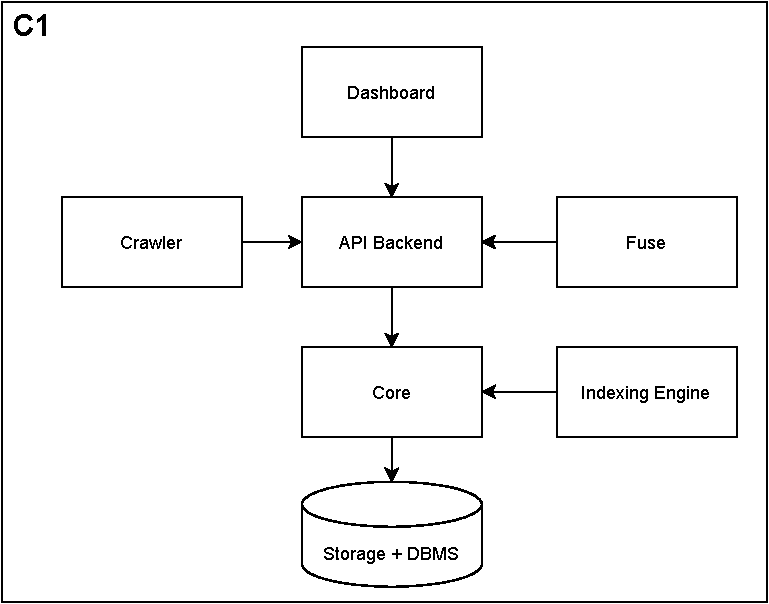
\includegraphics[width=1.0\textwidth, page={1}]{images/ComLake_arch.pdf}
    \caption{Level 1: System Context diagram: ComLake Overall Architecture diagram}
    \label{fig:C1}
\end{figure}
This is the System Context diagram for the ComLake system. The system comprises seven containers: a web application Dashboard, a server-side API Application, a data web Crawler, a Filesystem in USErspace (FUSE), an Image Indexing Engine using Machine Learning, a Core service that encapsulates distributed file system (DFS), and a database management system (DBMS).

The Dashboard, a ReactJS application that runs in the customer's web browser, will be the end-first user's point of contact. The Public API (API Backend in the figure) would handle authentication and authorization for external users and most internal services before being modified and given to the core API.

We will strive to build the Public API and Dashboard container. 

\section{Thesis Structure}
The thesis is divided into six main chapters to explain the development of Data Lake APIs and Dashboard.
\begin{itemize}
    \item The first chapter, Introduction, will discuss the fascinating subject of Data Lake APIs and Dashboards and the proposed solution in Chapter 1: Introduction.
    \item The second chapter, Objectives, we shall establish the project's standard requirements, present a quick summary of the system's operation, and present the reasons for its development.
    \item The third chapter, Requirement Analysis, will continue with the system's scenarios, use cases, object models, and dynamic models.
    \item The fourth chapter, Methodology, includes the entire functional specification and navigational paths that reflect the screen sequence. We will go through all of the tools and techniques utilized in the project, why they were chosen, and how the use cases were implemented in detail.
    \item The fifth chapter, Result and Discussion, we shall detail all of the functionalities that are implemented in the system
    \item The sixth chapter, Conclusions, provides conclusions about the project outcome and discusses the difficulties that exist during project development.
\end{itemize}


\chapter{Objectives}
\label{chap:object}
%---------------------------------------------------------
In this segment, we will define the standard requirements of the project, provide a brief overview of the function of the system and the reasons for its development.
\section{Desired Features}
The main goal of this project is to develop a Data Lake APIs and dashboard with basic services: 
\begin{itemize}
    \item \textbf{FEATURE 1: Authenticate}
    \begin{itemize}
        \item \textbf{SUB-FEATURE 1.1: Register}: allow users to create a new account
        \item \textbf{SUB-FEATURE 1.2: Login}: allow users to access into the system.
    \end{itemize}
    
    \item \textbf{FEATURE 2: Manage Users}
    \begin{itemize}
        \item \textbf{SUB-FEATURE 2.1: Create User}: allow Admin to create an account
        \item \textbf{SUB-FEATURE 2.2: View User}: 
            \begin{itemize}
                \item Allow Admin to get a list of all users in the system, filter users by their metadata, export users data to a CSV file
                \item Allow (Regular) User to view their own profile
            \end{itemize}
        \item \textbf{SUB-FEATURE 2.3: Update User}: 
            \begin{itemize}
                \item Allow Admin to edit users' information
                \item (Regular) User to update their own profile
            \end{itemize}
        \item \textbf{SUB-FEATURE 2.4: Delete User}: allow Admin to delete an account     
    \end{itemize}
    
    \item \textbf{FEATURE 3: Manage User Groups}
    \begin{itemize}
        \item \textbf{SUB-FEATURE 3.1: Create Group}: allow Admin to create a group
        \item \textbf{SUB-FEATURE 3.2: View Group}: allow Admin to get a list of all groups in the system, filter groups by their metadata, export groups data to a CSV file
        \item \textbf{SUB-FEATURE 3.3: Update Group}: allow Admin to add a user to a group
        \item \textbf{SUB-FEATURE 3.4: Delete Group}: allow Admin to delete a group
    \end{itemize}
    
    \item \textbf{FEATURE 4: Manage Folders}
    \begin{itemize}
        \item \textbf{SUB-FEATURE 4.1: Create Folder}: allow users to create a folder
        \item \textbf{SUB-FEATURE 4.2: View Folder}: 
            \begin{itemize}
                \item Admin can view all folders
                \item A (regular) User could only access folders they have permission to read
                \item Users can filter folders by their metadata, and export folders data to a CSV file
            \end{itemize}
        \item \textbf{SUB-FEATURE 4.3: Edit Folder}: 
            \begin{itemize}
                \item Admin can edit all folders
                \item A (regular) User could only edit folders they have permission to write
            \end{itemize}
        \item \textbf{SUB-FEATURE 4.4: Add a sub-folder to a folder}: 
        \begin{itemize}
            \item Admin can add all sub-folders to all folders
            \item A (regular) User could only add a sub-folder to a folder they have permission to write
        \end{itemize}
        \item \textbf{SUB-FEATURE 4.5: Delete Folder}:
            \begin{itemize}
                \item Admin can delete all folders
                \item A (regular) User could only delete folders they have permission to write
            \end{itemize}
    \end{itemize}
    
    \item \textbf{FEATURE 5: Manage Files}
    \begin{itemize}
        \item \textbf{SUB-FEATURE 5.1: Create File}: allow users to create a file
        \item \textbf{SUB-FEATURE 5.2: View File}: 
            \begin{itemize}
                \item Admin can view all files
                \item A (regular) User could only access files they have permission to read
                \item Users can filter files by their metadata, and export folders data to a CSV file
            \end{itemize}
        \item \textbf{SUB-FEATURE 5.3: Update File}: 
            \begin{itemize}
                \item Admin can edit all files
                \item A (regular) User could only edit files they have permission to write
            \end{itemize}
        \item \textbf{SUB-FEATURE 5.4: Add a file to a folder}: 
            \begin{itemize}
                \item Admin can add all files to all folders
                \item A (regular) User could only add files to folders they have permission to write
            \end{itemize}
        \item \textbf{SUB-FEATURE 5.5: Download File}: 
            \begin{itemize}
                \item Admin can add download all files
                \item A (regular) User could only download files they have permission to read
            \end{itemize}
        \item \textbf{SUB-FEATURE 5.6: Delete File}:
            \begin{itemize}
                \item Admin can delete all files
                \item A (regular) User could only delete files they have permission to write
            \end{itemize}
    \end{itemize}
    
    \item \textbf{FEATURE 6: Manage ACLs}
    \begin{itemize}
        \item \textbf{SUB-FEATURE 6.1: Grant ACL}: allow users to grant ACL (permission to read or write) to a user or a group for a file or folder
        \item \textbf{SUB-FEATURE 6.2: View ACL}: allow users to view all ACL (permission to read or write) of all folders or files they have access to; users could also search in ACL sources, filter ACLs based on their metadata, and export ACL data to a CSV file
        \item \textbf{SUB-FEATURE 6.3: Delete ACL}: allow users to remove ACL (permission to read or write) of a user or a group in a file or folder
    \end{itemize}
\end{itemize}
\section{Expected Outcome}
The system aims to create a Data Lake for all uses and storage of USTH and beyond the university. The specific goals include:
\begin{itemize}
    \item Develop a backend application that has all the desired features discussed and connected to the Data Lake Core
    \item Develop a web interface with interactions between users and the system
    \item The web page should be able to run in multiple browsers such as Chrome, Firefox, Safari 
\end{itemize}

%---------------------------------------------------------

%\section{Justification}


\chapter{Requirement Analysis}
\label{chap:requirement_analysis}
In this chapter, we will examine a brief review of the project's functions and the system's scenarios and use cases. This section includes the entire functional specification.

\section{Overall System Requirements}
In general, this application should satisfy the following requirements:
\begin{itemize}
  \item A login system with authentication
  \item Users can upload and download files
  \item The system limited users with some features
  \begin{itemize}
    \item For Admin:
        \begin{itemize}
            \item Manage Users
            \item Manage User Groups
            \item Access to all files and folders
            \item Grant or remove permissions for all files and folders
        \end{itemize}
    \item For Regular Users:
        \begin{itemize}
            \item View their own profile
            \item Update their own profile
            \item Access to files and folders they have permission to read and/or write
            \item Grant or remove permissions for the files or folders they own
        \end{itemize}
  \end{itemize}
\end{itemize}

\section{Users \& Non-functional Requirements}
\begin{itemize}
    \item \textbf{Users Requirement}: Have a device with internet access, preferable Chrome web browser
    \item \textbf{Performance}: The website is accessible by anyone with a public domain. 
    \item \textbf{Availability}: The user can only work with the system fully if they can login with a registered account.
    \item \textbf{Re-usability}: User can use external files with the website. User can use CSV file generated from the website for other purposes. The data generated by the website can be use as the resource for other services.
    \item \textbf{Reliability}: The system will not work without the Internet connection.
\end{itemize}

\section{Use Cases}
\subsection{Use Cases Diagram}
The following diagram describes the functions that a user can perform with the system.
\begin{figure}[H]
    \centering
    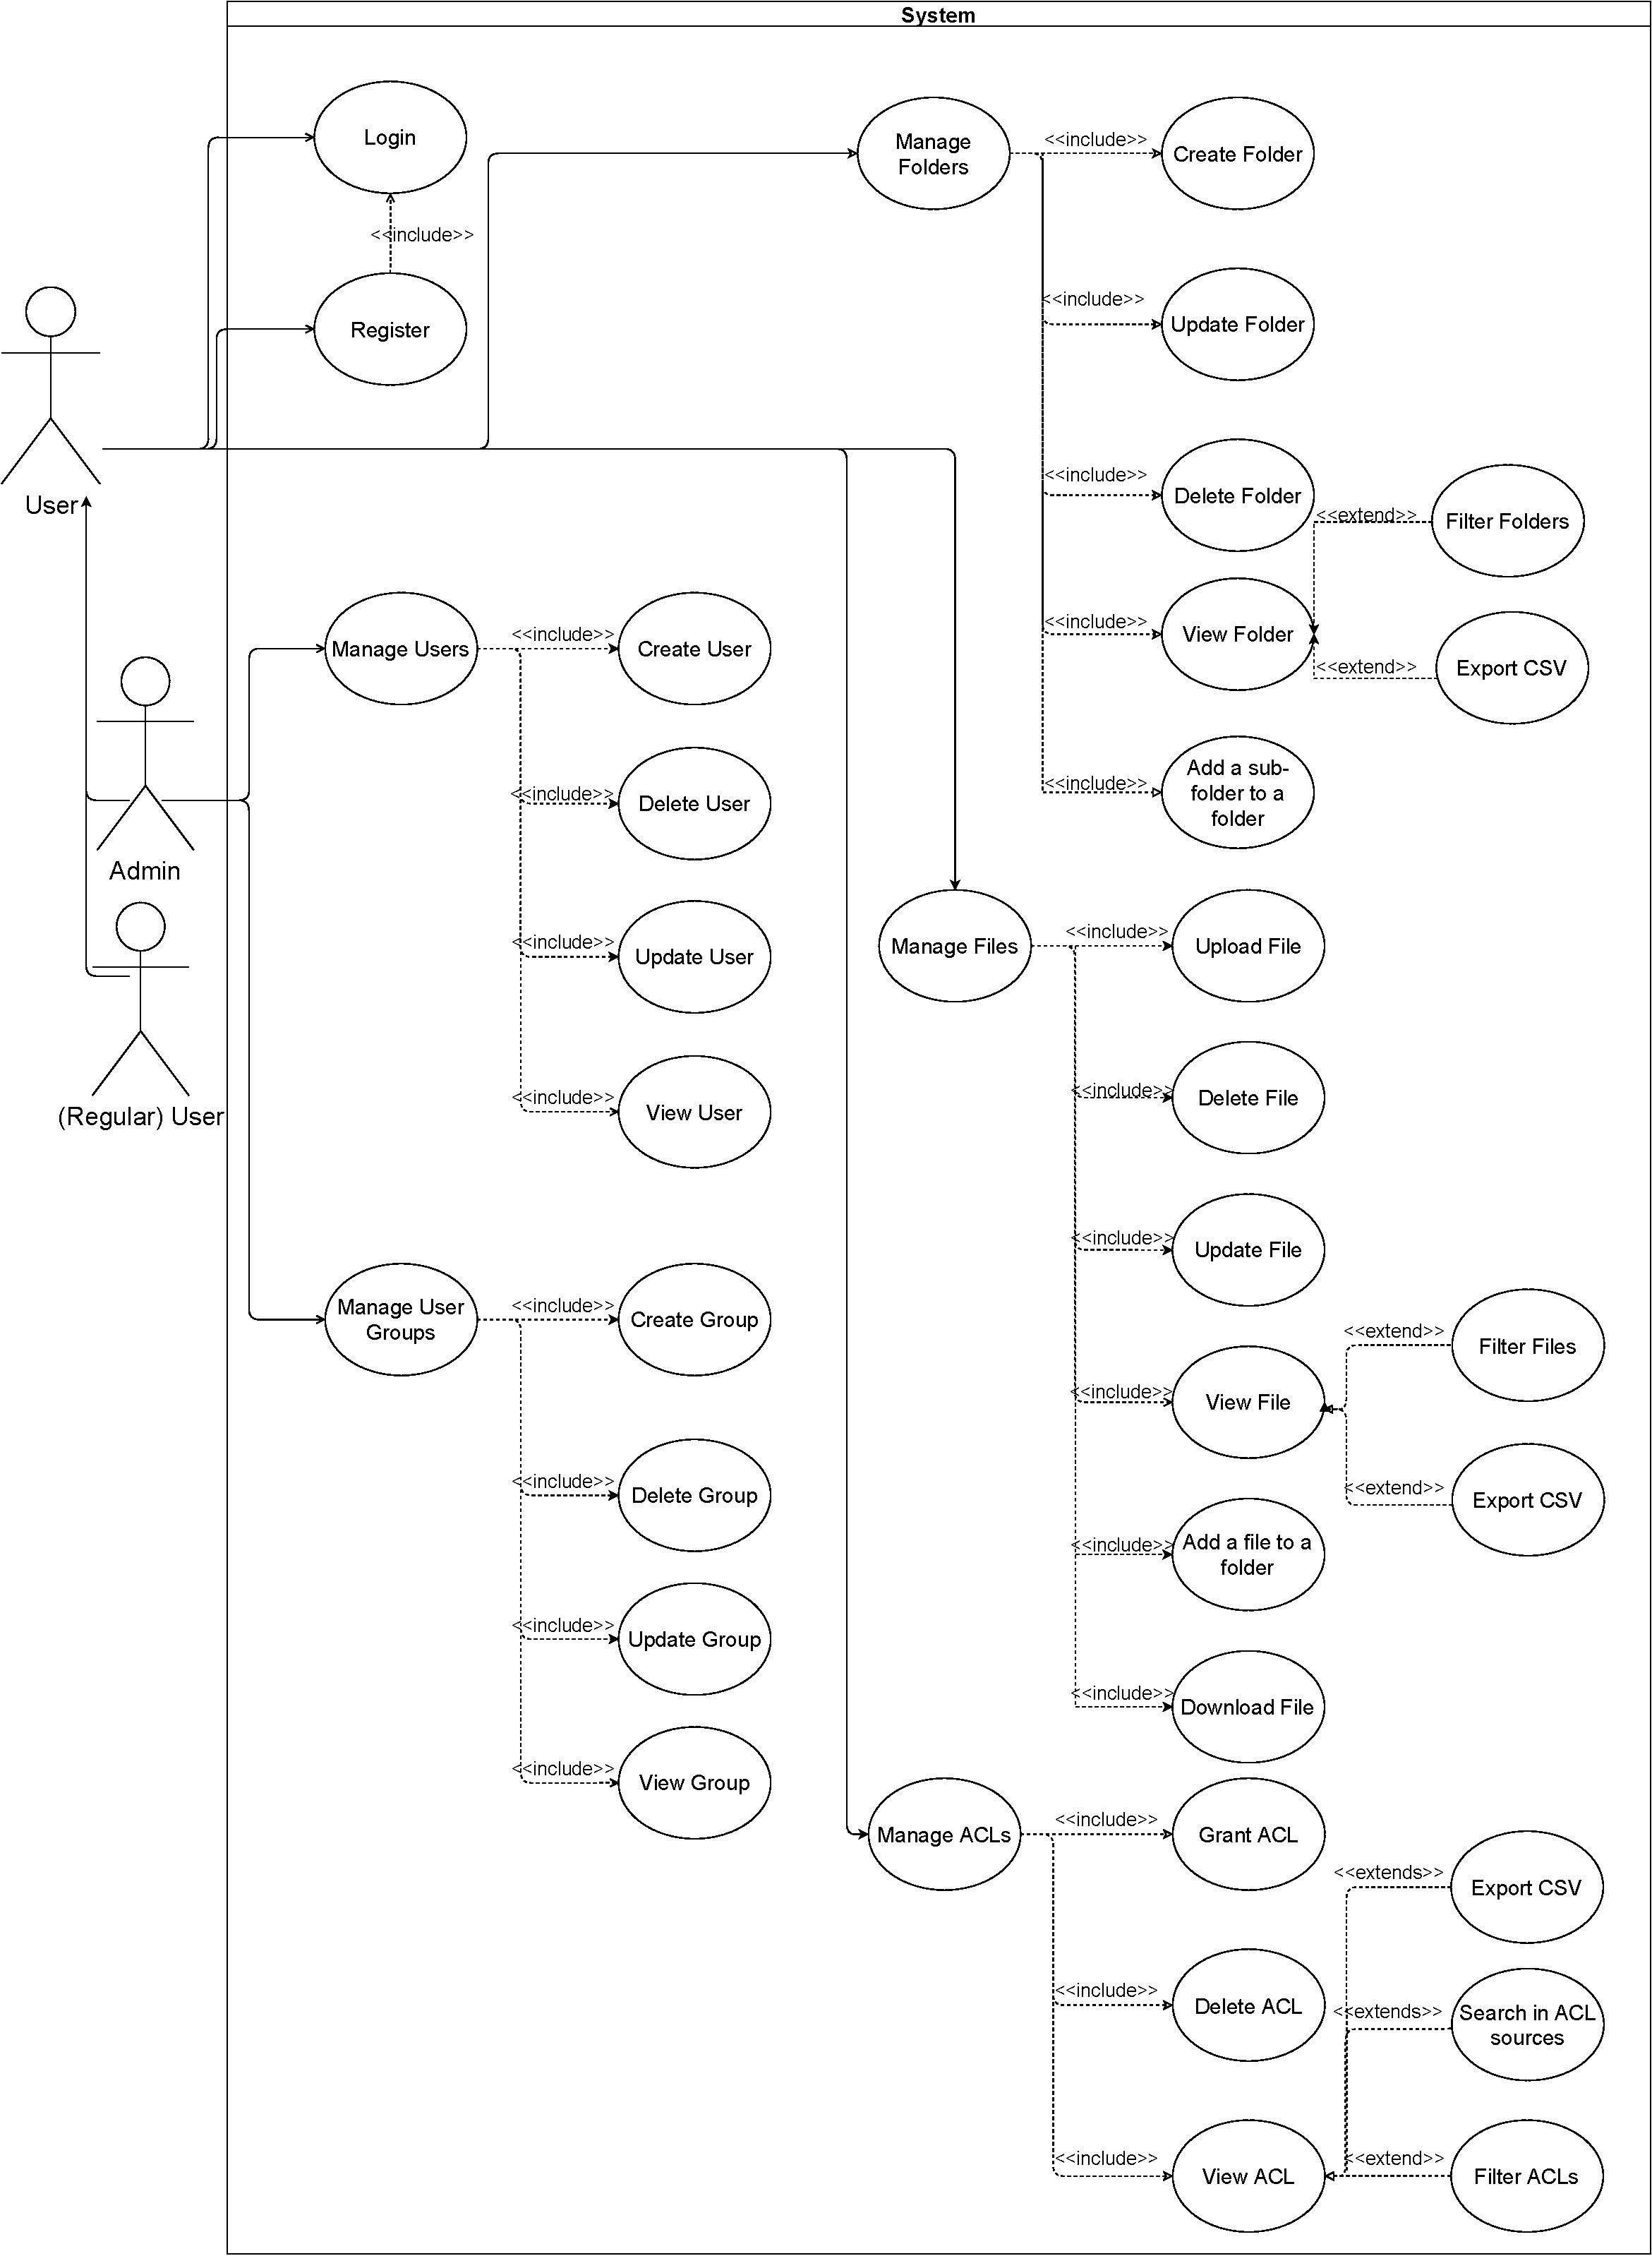
\includegraphics[width=0.95\textwidth]{images/Use_case_diagram_Top_level_All.pdf}
    \caption{Use cases diagram}
    \label{fig:description}
\end{figure}
\subsection{Users Characteristics}
Two types of users interact with the system: \textbf{Admin} and (regular) \textbf{User}. Each user type has different uses in the system, so each of them has its requirements:
\begin{itemize}
    \item \textbf{Admin}: a user who has access to all resources; only admin could manage user groups, total management of users
    \item \textbf{User}: a user who only has access to the resource they have permission to use, only could view and edit their profile.
\end{itemize}

\section{Use Case and Scenario Description}
\subsection{Use case: Register (SUB-FEATURE 1.1)}
\subsubsection{Brief description}
This use case describes how a user registers to the system. 
\subsubsection{Flow of events} 
\textbf{1. Basic Flow}

The table \ref{table:1} takes place when one person wants to create a new account on the system.
\begin{table}[H]
\centering
\begin{tabulary}{1.0\textwidth}{ |L|L|L| }
  \hline
    \rowcolor{gray} 
    \textbf{Actor Action} & 
    \textbf{System Action} & 
    \textbf{Data} \\
  \hline 
   & 1. The system requests that the Actor enter required information & - First name \newline- Last name \newline- Email \newline- Username \newline- Password \newline \\ 
  \hline
  2. The Actor enters their information. & 3. The system check the entered account exists on the system or not with username and email & \\
  \hline
  & 4. The system validates user’s information and create a new 
account for user and log the Actor into the system after created successfully & \\
  \hline 
\end{tabulary}
\caption{Register Basic Flow (SUB-FEATURE 1.1)}
\label{table:1}
\end{table}

\par
\textbf{2. Alternative Flows}

\begin{enumerate}[label=(\roman*)]
    \item Account exists \\
If in the Basic Flow, at step 3, the account has existed on the system, the system displays an error message. If the user goes back, return the form. The Actor can select to cancel the operation, at which point the Use Case ends.
    \item Invalid Format or Insufficient Information \\
If, in the Basic Flow, at step 2, the Actor has not specified sufficient information to create a new account as required, the system will prompt the Actor for the invalid field or the missing information. The Actor can either enter the missing information or cancel the operation, at which point the Use Case ends.
\end{enumerate}

\subsubsection{Special Requirement}
Only Regular Users can Register into the system. Admin is either pre-created or assigned an account. 
\subsubsection{Pre-conditions}
User is not logged in.
\subsubsection{Post-conditions}
If the use case is successful, the user registers successfully. If not, the system state is unchanged.

\subsection{Use case: Login (SUB-FEATURE 1.2)}
\subsubsection{Brief description}
The Use Case describes how a user logs into the system.
\subsubsection{Flow of events} 
\textbf{1. Basic Flow}
The table \ref{table:2} describe when the Actor wishes to Login to the system.
\begin{table}[H]
\centering
\begin{tabulary}{1.0\textwidth}{ |L|L|L| }
  \hline
    \rowcolor{gray} 
    \textbf{Actor Action} & 
    \textbf{System Action} & 
    \textbf{Data} \\
  \hline 
   & 1. The system requests that the Actor enter their username and password & - Username* \newline- Password* \newline* Required fields \\ 
  \hline
  2. The Actor enters their email and password. & 3. The system validates the entered name and password and logs the Actor into the system. & \\
  \hline 
\end{tabulary}
\caption{Login Basic Flow (SUB-FEATURE 1.2)}
\label{table:2}
\end{table}

\par
\textbf{2. Alternative Flows}

\begin{enumerate}[label=(\roman*)]
    \item Invalid Username/Password \\
If in the Basic Flow, at step 2, the Actor enters an invalid username or password, the system displays an error message. The Actor can either return to the beginning of the Basic Flow or cancel the login, at which point the Use Case ends.
\end{enumerate}

\subsubsection{Special Requirement}
None.
\subsubsection{Pre-conditions}
The user account must exist.
\subsubsection{Post-conditions}
If the Use Case was successful, the Actor is now logged into the system. If not, the system state is unchanged.

\subsection{Use case: Manage Users (FEATURE 2)}
\subsubsection{Brief description}
The Use Case allows the system Admin to manage users' information. This includes adding a new user to the system, changing existing users' information on the system, removing a user from the system, and viewing a user.
\subsubsection{Flow of events} 
\textbf{1. Basic Flow}
The table \ref{table:3} describe when the Admin wishes to add, change, and/or delete User information in the system.
\begin{table}[H]
\centering
\begin{tabulary}{1.0\textwidth}{ |L|L|L| }
  \hline
    \rowcolor{gray} 
    \textbf{Actor Action} & 
    \textbf{System Action} & 
    \textbf{Data} \\
   \hline 
  1. The Admin wants to manage users. & 2. The system shows list of all users. & List of all users details.\\
  \hline 
  3. The Admin views the users lists and/or filers them by custom criteria. & 4. The system displays the users by custom criteria. & List of all users with custom criteria.\\
  \hline
  & 5. The system requests that the Admin specifies  the function he/she would like to perform (either Create a User, Update User or Delete User). & - Manage selection \\ 
  \hline
  6. The Admin selects "Create User". & 7. The system requests the
Administrator to enter the User information. &  - Username* \newline- Password* \newline- Email* \newline- First Name \newline- Last Name \newline- Department \newline- Affiliation \newline* Required fields \\
  \hline 
  8. The Admin provides the requested information. & 9. The system generates and assigns a unique User Id number to the user. The User is added to the system.  & \\
  \hline 
\end{tabulary}
\caption{Manage Users Basic Flow (SUB-FEATURE 2.1 \& SUB-FEATURE 2.2)}
\label{table:3}
\end{table}

\emph{Update User Sub Flow} \par
At step 6 of \textbf{Basic Flow }
\begin{table}[H]
\centering
\begin{tabulary}{1.0\textwidth}{ |L|L|L| }
  \hline
    \rowcolor{gray} 
    \textbf{Actor Action} & 
    \textbf{System Action} & 
    \textbf{Data} \\
  \hline 
  1. The Admin selects "Update User". & 2. The system requests the Admin to select User from User list or User profile interface. & \\ 
  \hline
  3. The Admin selects User. & 4. The system retrieves and displays the User. &  \\
  \hline 
  5. The Admin enter the desired changes to the User information. & 6. The system updates the User record with the updated information. & \newline- First Name \newline- Last Name \newline- Department \newline- Affiliation \\
  \hline 
\end{tabulary}
\caption{Update User Sub Flow (SUB-FEATURE 2.3)}
\label{table:5}
\end{table}

\emph{Delete User Sub Flow} \par
At step 6 of \textbf{Basic Flow }
\begin{table}[H]
\centering
\begin{tabulary}{1.0\textwidth}{ |L|L|L| }
  \hline
    \rowcolor{gray} 
    \textbf{Actor Action} & 
    \textbf{System Action} & 
    \textbf{Data} \\
  \hline 
  1. The Admin selects "Delete User". & 2. The system requests the Admin to select User from User list or User profile interface. & \\ 
  \hline
  3. The Admin selects User. & 4. The system retrieves and displays the User. &  \\
  \hline 
  5. The Admin select delete. & 6. The system removes the User from the system.& \\
  \hline 
\end{tabulary}
\caption{Delete User Sub Flow (SUB-FEATURE 2.4)}
\label{table:4}
\end{table}

\par
\textbf{2. Alternative Flows}

\begin{enumerate}[label=(\roman*)]
    \item User not found \\
If in the Update User sub flow, at step 3 or Delete User sub flow, at step 3, a User with the specified id number does not exist, the system displays an error message. The Administrator can cancel the operation, at which point the Use Case ends.
\end{enumerate}

\subsubsection{Special Requirement}
None.
\subsubsection{Pre-conditions}
The Admin must be logged into the system before this Use Case begins.
\subsubsection{Post-conditions}
If the Use Case was successful, the User information is created, updated, deleted from the system. Otherwise, the system state is unchanged.

\subsection{Use case: Manage User Groups (FEATURE 3)}
\subsubsection{Brief description}
The Use Case allows the system Admin to manage user groups' information. This includes adding a new group to the system, changing existing group' information on the system, removing a group from the system, and viewing a group.
\subsubsection{Flow of events} 
\textbf{1. Basic Flow}
The table \ref{table:6} describe when the Admin wishes to add, change, and/or delete Group information in the system.
\begin{table}[H]
\centering
\begin{tabulary}{1.0\textwidth}{ |L|L|L| }
  \hline
    \rowcolor{gray} 
    \textbf{Actor Action} & 
    \textbf{System Action} & 
    \textbf{Data} \\
   \hline 
  1. The Admin wants to manage groups. & 2. The system shows list of all groups. & List of all groups details.\\
  \hline 
  3. The Admin views the groups lists and/or filter groups by custom criteria. & 4. The system displays the groups by custom criteria. & List of all groups with custom criteria.\\
  \hline
  & 5. The system requests that the Admin specify the function he/she would like to perform (either Create a Group, Update Group or Delete Group). & Manage selection \\ 
  \hline
  6. The Admin selects "Create Group". & 7. The system requests the
Administrator to enter the User information. & Name* \\
  \hline 
  8. The Admin provides the requested information. & 9. The system generates and assigns a unique Group Id number to the user. The Group is added to the system.  & \\
  \hline 
\end{tabulary}
\caption{Manage Groups Basic Flow (SUB-FEATURE 3.1 \& SUB-FEATURE 3.1)}
\label{table:6}
\end{table}

\emph{Update Group Sub Flow} \par
At step 6 of \textbf{Basic Flow }
\begin{table}[H]
\centering
\begin{tabulary}{1.0\textwidth}{ |L|L|L| }
  \hline
    \rowcolor{gray} 
    \textbf{Actor Action} & 
    \textbf{System Action} & 
    \textbf{Data} \\
  \hline 
  1. The Admin selects "Update Group". & 2. The system requests the Admin to select Group from Group list or Group details interface. & \\ 
  \hline
  3. The Admin selects Group. & 4. The system retrieves and displays the Group along with a list of all users. &  \\
  \hline 
  5. The Admin adds a user from User list to a group. & 6. The system updates the Group record with the updated information. &  Username  \\
  \hline 
\end{tabulary}
\caption{Update Group Sub Flow (SUB-FEATURE 3.3)}
\label{table:8}
\end{table}

\emph{Delete Group Sub Flow} \par
At step 6 of \textbf{Basic Flow }
\begin{table}[H]
\centering
\begin{tabulary}{1.0\textwidth}{ |L|L|L| }
  \hline
    \rowcolor{gray} 
    \textbf{Actor Action} & 
    \textbf{System Action} & 
    \textbf{Data} \\
  \hline 
  1. The Admin selects "Delete Group". & 2. The system requests the Admin to select Group from Group list or Group details interface. & \\ 
  \hline
  3. The Admin selects Group. & 4. The system retrieves and displays the Group. &  \\
  \hline 
  5. The Admin select delete. & 6. The system removes the Group from the system.& \\
  \hline 
\end{tabulary}
\caption{Delete Group Sub Flow (SUB-FEATURE 3.4)}
\label{table:7}
\end{table}
\par
\textbf{2. Alternative Flows}

\begin{enumerate}[label=(\roman*)]
    \item Group not found \\
If in the Update Group sub flow, at step 3 or Delete Group sub flow, at step 3, a Group with the specified id number does not exist, the system displays an error message. The Administrator can cancel the operation, at which point the Use Case ends.
\end{enumerate}

\subsubsection{Special Requirement}
None.
\subsubsection{Pre-conditions}
The Admin must be logged into the system before this Use Case begins.
\subsubsection{Post-conditions}
If the Use Case was successful, the Group information is created, updated, deleted from the system. Otherwise, the system state is unchanged.

\subsection{Use case: Manage Folders (FEATURE 4)}
\subsubsection{Brief description}
The Use Case allows the system users to manage folders' information. This includes adding a new folder to the system, changing existing folders' information on the system, removing a folder from the system, and viewing a folder.
\subsubsection{Flow of events} 
\textbf{1. Basic Flow}
The table \ref{table:9} describe when the users wish to add, change, and/or delete Folder information in the system.
\begin{table}[H]
\centering
\begin{tabulary}{1.0\textwidth}{ |L|L|L| }
  \hline
    \rowcolor{gray} 
    \textbf{Actor Action} & 
    \textbf{System Action} & 
    \textbf{Data} \\
   \hline 
  1. The users want to manage folders. & 2. The system shows the list of all folders and files details. & \\
  \hline 
  3. The users view the folders and files lists and/or filter them by custom criteria. & 4. The system displays the files and folders by custom criteria. & List of all files and folders with custom criteria.\\
  \hline
  & 5. The system requests that the users specify the function he/she would like to perform (either Create a Folder, Update Folder, Move Folder, or Delete Folder). & - Manage selection \\ 
  \hline
  6. The users select "Create Folder". & 7. The system requests the
users to enter the Folder information. &  - Name* \newline- Source* \newline- Topics* \newline* Required fields \\
  \hline 
  8. The users provide the requested information. & 9. The system generates and assigns a unique Folder Id number to the User. The Folder is added to the system.  The User is recognized as the Folder's owner by the system with read and write permission. Permission for Admin is also automatically added. & \\
  \hline 
\end{tabulary}
\caption{Manage Folders Basic Flow (SUB-FEATURE 4.1 \&  SUB-FEATURE 4.2)}
\label{table:9}
\end{table}

\emph{Edit Folder Sub Flow} \par
At step 6 of \textbf{Basic Flow }
\begin{table}[H]
\centering
\begin{tabulary}{1.0\textwidth}{ |L|L|L| }
  \hline
    \rowcolor{gray} 
    \textbf{Actor Action} & 
    \textbf{System Action} & 
    \textbf{Data} \\
  \hline 
  1. The users select "Update Folder". & 2. The system requests the users to select Folder from Folder list or Folder details interface. & \\ 
  \hline
  3. The users select Folder. & 4. The system retrieves and displays the Folder. &  \\
  \hline 
  5. The users enter the desired changes to the Folder information. & 6. The system updates the Folder record with the updated information. & \newline- Name \newline- Source \newline- Topics \\
  \hline 
\end{tabulary}
\caption{Edit Folder Sub Flow (SUB-FEATURE 4.3)}
\label{table:11}
\end{table}
\par

\emph{Move a Sub-folder to a Folder Sub Flow} \par
At step 6 of \textbf{Basic Flow}
\begin{table}[H]
\centering
\begin{tabulary}{1.0\textwidth}{ |L|L|L| }
  \hline
    \rowcolor{gray} 
    \textbf{Actor Action} & 
    \textbf{System Action} & 
    \textbf{Data} \\
  \hline 
1. The users select "Move Folder". & 2. The system requests the users to select Folder from Folder list or Folder details interface. & \\ 
  \hline
3. The users select Folder. & 4. The system retrieves and displays the Folder. &  \\
  \hline 
5. The users enter the destination folder name. & 6. The system updates the Folder record with the updated information. & Destination Folder name \\
  \hline 
\end{tabulary}
\caption{Move a sub-folder to a Folder Sub Flow (SUB-FEATURE 4.4)}
\label{table:12}
\end{table}
\par

\emph{Delete Folder Sub Flow} \par
At step 6 of \textbf{Basic Flow }
\begin{table}[H]
\centering
\begin{tabulary}{1.0\textwidth}{ |L|L|L| }
  \hline
    \rowcolor{gray} 
    \textbf{Actor Action} & 
    \textbf{System Action} & 
    \textbf{Data} \\
  \hline 
  1. The users selects "Delete Folder". & 2. The system requests the users to select Folder from Folder list or Folder details interface. & \\ 
  \hline
  3. The users selects Folder. & 4. The system retrieves and displays the Folder. &  \\
  \hline 
  5. The users select delete. & 6. The system removes the Folder from the system.& \\
  \hline 
\end{tabulary}
\caption{Delete Folder Sub Flow (SUB-FEATURE 4.5)}
\label{table:10}
\end{table}
\par

\textbf{2. Alternative Flows}

\begin{enumerate}[label=(\roman*)]
    \item Folder not found \\
If in the Update Folder sub flow, at step 3 or Delete Folder sub flow, at step 3, a Folder with the specified id number does not exist, the system displays an error message. The users can cancel the operation, at which point the Use Case ends.
    \item Invalid Format or Insufficient Information\\
If, in the Create Folder sub flow, at step 7; in the Edit Folder and Move Folder sub flow, at step 5, the users have not specified sufficient information to add a new Folder, the system will prompt the users for the missing information. The users can either enter the missing information or choose to cancel the operation, at which point the Use Case ends.
    \item The users do not have the permission to view\\
If, in the Basic Flow at step 2, the users do not have the right to view a folder. The folder doesn't appear in the list of all files and folders.
    \item The users do not have the permission to write\\
If, in the Edit Folder, Move Folder and Delete Folder sub flow, at step 5, the users do not have the right to write folder. The users can choose to cancel the operation, at which point the Use Case ends.
\end{enumerate}

\subsubsection{Special Requirement}
None.
\subsubsection{Pre-conditions}
The users must be logged into the system before this Use Case begins.
\subsubsection{Post-conditions}
If the Use Case was successful, the Folder information is created, updated, deleted from the system. Otherwise, the system state is unchanged.

\subsection{Use case: Manage Files (FEATURE 5)}
\subsubsection{Brief description}
The Use Case allows the system users to manage files' information. This includes upload a new file to the system, changing existing files' information on the system, removing a file from the system, and viewing a file.
\subsubsection{Flow of events} 
\textbf{1. Basic Flow}
The table \ref{table:13} describe when the users wish to upload, change, and/or delete File information in the system.
\begin{table}[H]
\centering
\begin{tabulary}{1.0\textwidth}{ |L|L|L| }
  \hline
    \rowcolor{gray} 
    \textbf{Actor Action} & 
    \textbf{System Action} & 
    \textbf{Data} \\
   \hline 
  1. The users want to manage files. & 2. The system shows the list of all folders and files details. &\\
  \hline 
  3. The users view the folders and files lists and/or filter them by custom criteria. & 4. The system displays the files and folders by custom criteria. & List of all files and folders with custom criteria.\\
  \hline
  & 5. The system requests that the users specify the function he/she would like to perform (either Create a File, Update File, Move File, Download File, or Delete File). & - Manage selection \\ 
  \hline
  6. The users select "Upload File". & 7. The system requests the
users to enter the File information. &  - File(s) Data* \newline- Source* \newline- Topics* \newline* Required fields \\
  \hline 
  8. The users provide the requested information. & 9. The system generates and assigns a unique File Id number to the User. The File is uploaded to the system.  The User is recognized as the File's owner by the system with read and write permission. Permission for Admin is also automatically uploaded. & \\
  \hline 
\end{tabulary}
\caption{Manage Files Basic Flow (SUB-FEATURE 5.1 \& SUB-FEATURE 5.2)} 
\label{table:13}
\end{table}

\emph{Edit File Sub Flow} \par
At step 6 of \textbf{Basic Flow }
\begin{table}[H]
\centering
\begin{tabulary}{1.0\textwidth}{ |L|L|L| }
  \hline
    \rowcolor{gray} 
    \textbf{Actor Action} & 
    \textbf{System Action} & 
    \textbf{Data} \\
  \hline 
  1. The users select "Update File". & 2. The system requests the users to select File from File list or File details interface. & \\ 
  \hline
  3. The users select File. & 4. The system retrieves and displays the File. &  \\
  \hline 
  5. The users enter the desired changes to the File information. & 6. The system updates the File record with the updated information. & \newline- Name \newline- Source \newline- Topics \\
  \hline 
\end{tabulary}
\caption{Update File Sub Flow (SUB-FEATURE 5.3)}
\label{table:15}
\end{table}
\par

\emph{Add a File to a Folder Sub Flow} \par
At step 6 of \textbf{Basic Flow }
\begin{table}[H]
\centering
\begin{tabulary}{1.0\textwidth}{ |L|L|L| }
  \hline
    \rowcolor{gray} 
    \textbf{Actor Action} & 
    \textbf{System Action} & 
    \textbf{Data} \\
  \hline 
1. The users select "Move File". & 2. The system requests the users to select File from File list or File details interface. & \\ 
  \hline
3. The users select File. & 4. The system retrieves and displays the File. &  \\
  \hline 
5. The users enter the destination folder name. & 6. The system updates the File record with the updated information. & Destination File name \\
  \hline 
\end{tabulary}
\caption{Add a File to a Folder Sub Flow (SUB-FEATURE 5.4)}
\label{table:16}
\end{table}
\par

\emph{Download File Sub Flow} \par
At step 6 of \textbf{Basic Flow }
\begin{table}[H]
\centering
\begin{tabulary}{1.0\textwidth}{ |L|L|L| }
  \hline
    \rowcolor{gray} 
    \textbf{Actor Action} & 
    \textbf{System Action} & 
    \textbf{Data} \\
  \hline 
1. The users select "Download File". & 2. The system requests the users to select File from files and folders list or File details interface. & \\ 
  \hline
3. The users select File. & 4. The system retrieves and displays the File. &  \\
  \hline 
5. The users select to download File. & 6. The system return the File data. & File Data \\
  \hline 
\end{tabulary}
\caption{Download File Sub Flow (SUB-FEATURE 5.5)}
\label{table:17}
\end{table}
\par

\emph{Delete File Sub Flow} \par
At step 6 of \textbf{Basic Flow }
\begin{table}[H]
\centering
\begin{tabulary}{1.0\textwidth}{ |L|L|L| }
  \hline
    \rowcolor{gray} 
    \textbf{Actor Action} & 
    \textbf{System Action} & 
    \textbf{Data} \\
  \hline 
  1. The users selects "Delete File". & 2. The system requests the users to select File from File list or File details interface. & \\ 
  \hline
  3. The users selects File. & 4. The system retrieves and displays the File. &  \\
  \hline 
  5. The users select delete. & 6. The system removes the File from the system.& \\
  \hline 
\end{tabulary}
\caption{Delete File Sub Flow (SUB-FEATURE 5.6)}
\label{table:14}
\end{table}
\par
\textbf{2. Alternative Flows}

\begin{enumerate}[label=(\roman*)]
    \item File not found \\
If in the Update File sub flow, at step 3 or Delete File sub flow, at step 3, a File with the specified id number does not exist, the system displays an error message. The users can cancel the operation, at which point the Use Case ends.
    \item Invalid Format or Insufficient Information\\
If, in the Upload File sub flow, at step 7; in the Edit File and Move File sub flow, at step 5, the users have not specified sufficient information to upload new File, the system will prompt the users for the missing information. The users can either enter the missing information or choose to cancel the operation, at which point the Use Case ends.
    \item The users do not have the permission to view\\
If, in the Basic Flow at step 2, and in the Download File sub flow at step 5, the users do not have the right to view a file. The file doesn't appear in the list of all files and folders. And the users can't download the file. 
    \item The users do not have the permission to write\\
If, in the Edit File, Move a File to a Folder and Delete File sub flow, at step 5, the users do not have the right to write folder. The users can choose to cancel the operation, at which point the Use Case ends.
\end{enumerate}

\subsubsection{Special Requirement}
None.
\subsubsection{Pre-conditions}
The users must be logged into the system before this Use Case begins.
\subsubsection{Post-conditions}
If the Use Case was successful, the File information is created, updated, deleted from the system. Otherwise, the system state is unchanged.

\subsection{Use case: Manage ACLs (FEATURE 6)}
\subsubsection{Brief description}
The Use Case allows the system users to manage ACLs' information. This includes adding a new ACL to the system, changing existing ACLs' information on the system, removing a ACL from the system, and viewing a ACL.
\subsubsection{Flow of events} 
\textbf{1. Basic Flow}
The table \ref{table:18} describe when the users wish to add, change, and/or delete ACL information in the system.
\begin{table}[H]
\centering
\begin{tabulary}{1.0\textwidth}{ |L|L|L| }
  \hline
    \rowcolor{gray} 
    \textbf{Actor Action} & 
    \textbf{System Action} & 
    \textbf{Data} \\
   \hline 
  1. The users want to manage ACLs. & 2. The system shows the list of all ACLs details of the selected file or folder. & \\
  \hline
  & 3. The system requests that the users specify the function he/she would like to perform (either Grant a ACL, or Delete ACL). & - Manage selection \\ 
  \hline
  4. The users select "Grant ACL". & 5. The system requests the users to enter the ACL information. &  - Source Name* \newline- Target Id* \newline- Source Type (File or Folder)* \newline- Target Type (User or Group)* \newline- Permission (Read or Write)* \newline* Required fields \\
  \hline 
  6. The users provide the requested information. & 7. The system generates and assigns a ACL permission to the source. The ACL permission is added to the system.  &  \\
  \hline
\end{tabulary}
\caption{Manage ACLs Basic Flow (SUB-FEATURE 6.1 \& SUB-FEATURE 6.2)}
\label{table:18}
\end{table}

\emph{Delete ACL Sub Flow} \par
At step 3 of \textbf{Basic Flow }
\begin{table}[H]
\centering
\begin{tabulary}{1.0\textwidth}{ |L|L|L| }
  \hline
    \rowcolor{gray} 
    \textbf{Actor Action} & 
    \textbf{System Action} & 
    \textbf{Data} \\
  \hline 
  1. The users selects "Delete ACL". & 2. The system requests the users to select ACL from ACL list. & \\ 
  \hline
  3. The users select delete. & 4. The system removes the ACL from the system.& \\
  \hline 
\end{tabulary}
\caption{Delete ACL Sub Flow (SUB-FEATURE 6.3)}
\label{table:19}
\end{table}
\textbf{2. Alternative Flows}

\begin{enumerate}[label=(\roman*)]
    \item ACL not found \\
If in Delete ACL sub flow, at step 3, a ACL with the specified id number does not exist, the system displays an error message. The users can cancel the operation, at which point the Use Case ends.
    \item The users do not have the permission to view\\
If, in the Basic Flow at step 2, the users do not have the right to view a file or a folder. They can not know the file or folder permission details. 
    \item The users do not have the permission to write\\
If, in the Delete sub flow, at step 2, the users do not have the right to write the selected file or folder. The users can choose to cancel the operation, at which point the Use Case ends.
    \item Invalid Format or Insufficient Information\\
If, in the Grant ACL sub flow, at step 5; the users have not specified sufficient information to add a new ACL, the system will prompt the users for the missing information. The users can either enter the missing information or choose to cancel the operation, at which point the Use Case ends.
\end{enumerate}

\subsubsection{Special Requirement}
None.
\subsubsection{Pre-conditions}
The users must be logged into the system before this Use Case begins.
\subsubsection{Post-conditions}
If the Use Case was successful, the ACL information is created or deleted from the system. Otherwise, the system state is unchanged.


\chapter{Methodology}
\label{chap:methods}
In this section, we will list all the tools and techniques used in this project, the reasons why they are chosen with overall system architecture and the detailed use cases implementations.

\section{System Architecture}
Here, we will continue from the figure \ref{fig:C1} as stated in the Introduction, zooming in to each container and component to see the details of the system architecture.

\paragraph{Level 2: Container diagram}

This is the Container diagram for ComLake Sytem. It shows that the application is made up of 3 containers: a web application Dashboard, a server-side API Application, and a Database. The Dashboard is an ReactJS application that runs in the user's web browser, providing all of the ComLake features. The Dashboard Web Application uses a JSON/HTTP API, which is provided by another Java/Spring MVC application running on the server. The Backend API Application gets user information and other information from the Database (MySQL).

\begin{figure}[H]
    \centering
    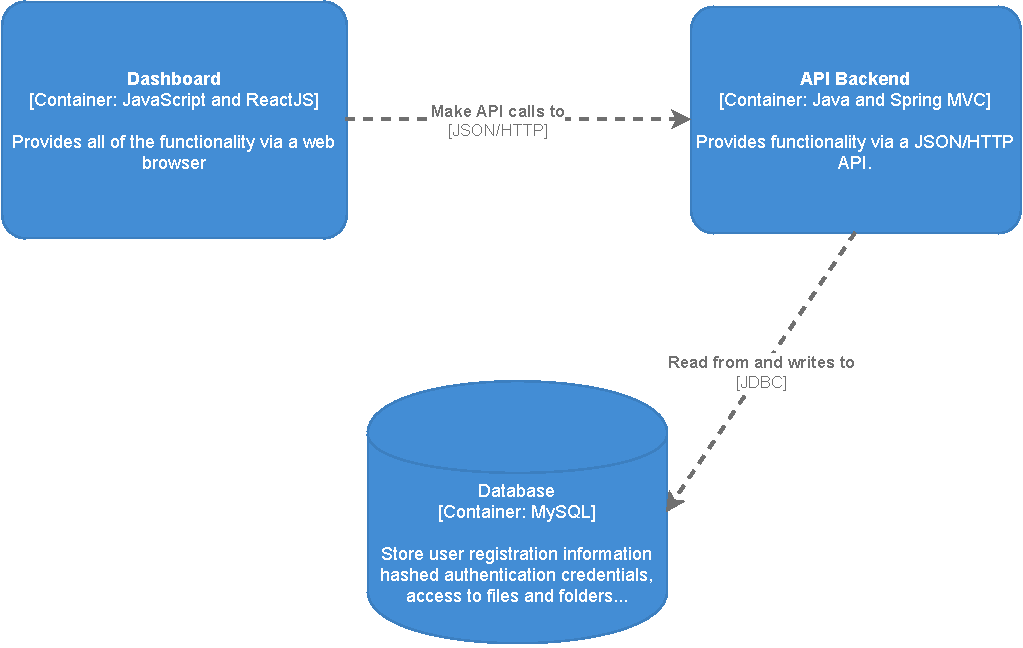
\includegraphics[width=1.0\textwidth]{images/C2.pdf}
    \caption{Container diagram for ComLake System - Backend API and Dashboard}
    \label{fig:C2}
\end{figure}

\paragraph{Level 3: Component diagram}
This is the Component diagram for ComLake system, showing some of the components within the Backend API application. Here, there are six Spring MVC Rest Controllers providing access points for the JSON/HTTP API, with each controller subsequently using other components to access data from the Database.
\begin{figure}[H]
    \centering
    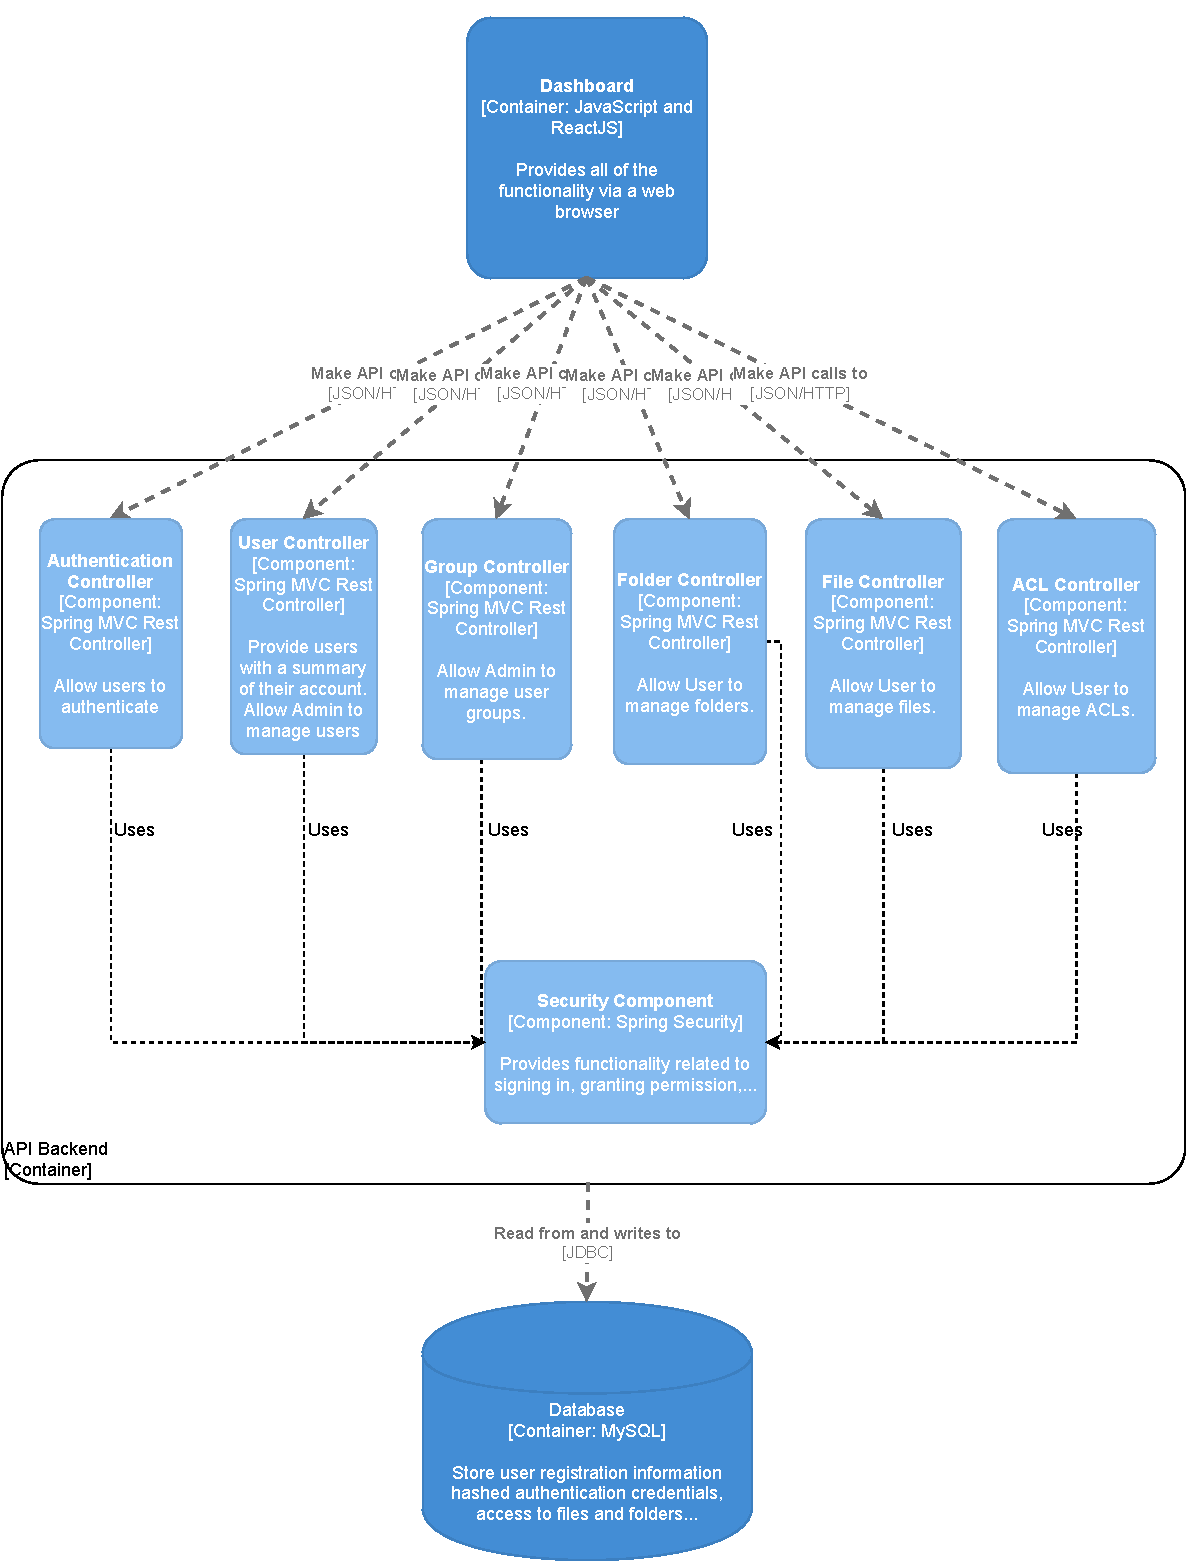
\includegraphics[width=0.9\textwidth]{images/C3.pdf}
    \caption{Component diagram for ComLake Sytem - Backend API}
    \label{fig:C3}
\end{figure}

\paragraph{Level 4: Code}
Finally, this is how the API Backend is implemented as code. This package contains classes for major processing functionality within the system. Control classes exist to support authentication management, user management, user group management, permission management, file and folder management.
\begin{figure}[H]
    \centering
    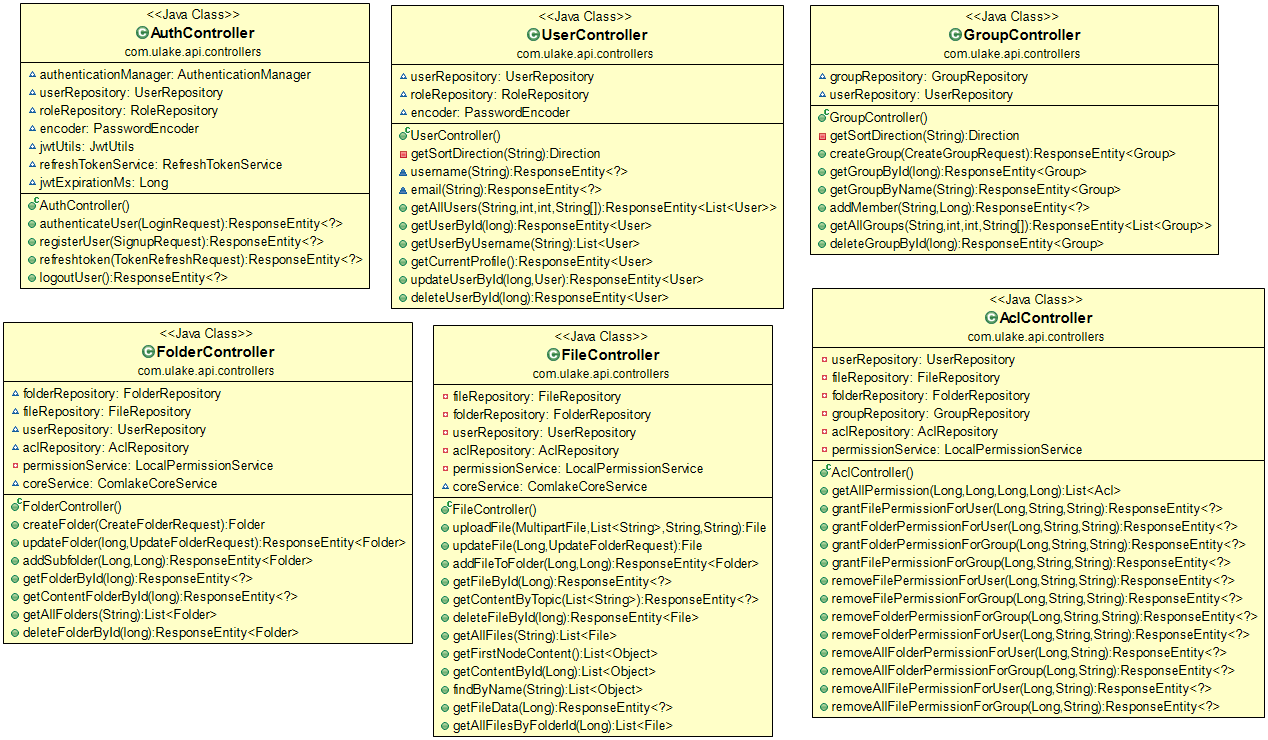
\includegraphics[width=1.0\textwidth]{images/package.png}
    \caption{API Backend Application Package Class diagram}
    \label{fig:C4}
\end{figure}

\section{Database Design}
Every table has the prefix "clake" to distinguish different services of the ComLake service from each other. 

\begin{figure}[H]
    \centering
    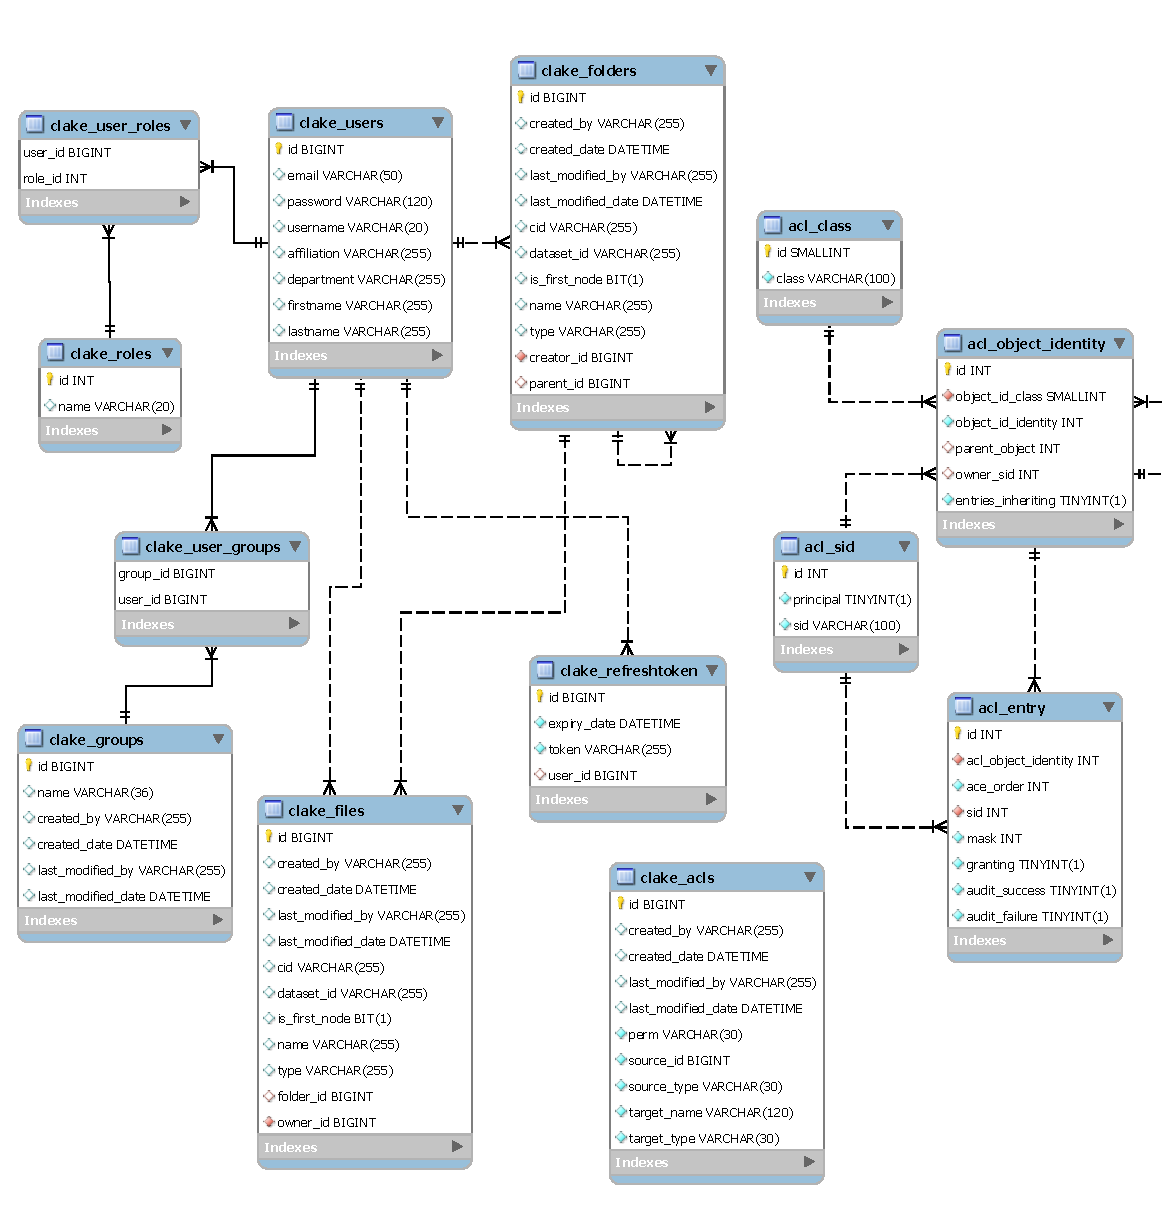
\includegraphics[width=1.0\textwidth]{images/OverallDatabaseDesign.pdf}
    \caption{Overall Database Design}
    \label{fig:DatabaseDesign}
\end{figure}

\begin{table}[H]
  \centering
  \caption{Database User Design}
  \label{tbl:dbUser}
  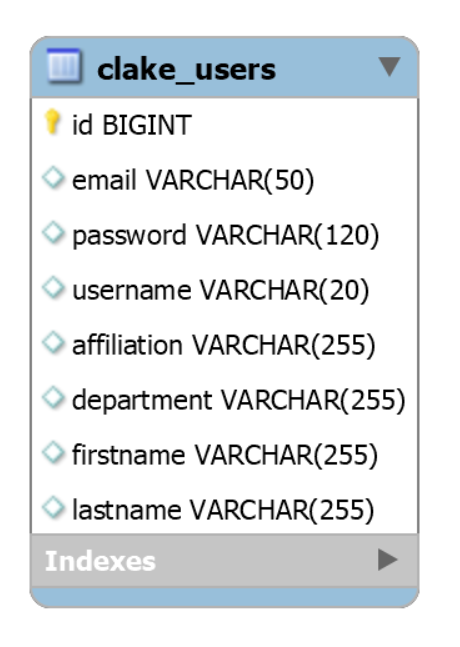
\includegraphics[width=0.3\textwidth]{images/DatabaseUserDesign.PNG}
\end{table}
\begin{itemize}
    \item "clake\_users" is the table that contains the information of accounts. This table has sensitive data of users such as "password". 
    \item The 'password' field in this table is saved in an encrypted form not easily used by attackers. 
    \item After the user register, the system saves the user information and assign a unique "id" to the user, and this "id" is the Primary key of the table. 
\end{itemize}

\begin{table}[H]
  \centering
  \caption{Database Role Design}
  \label{tbl:dbRole}
  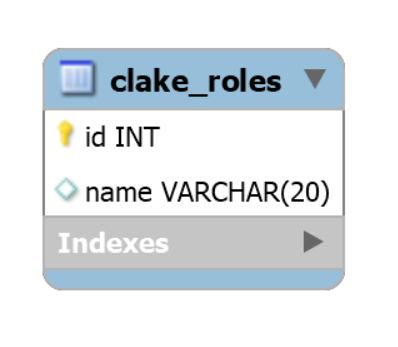
\includegraphics[width=0.3\textwidth]{images/DatabaseRoleDesign.PNG}
\end{table}
\begin{itemize}
    \item "clake\_roles" is the table that contains the information of roles, for example role name. 
    \item In this system, we only have 2 role. Role Admin and role (Regular) User.
    \item This table has "id" as Primary Key. Each role has an unique "id". 
\end{itemize}

\begin{table}[H]
  \centering
  \caption{Database User Role Design}
  \label{tbl:dbUserRole}
  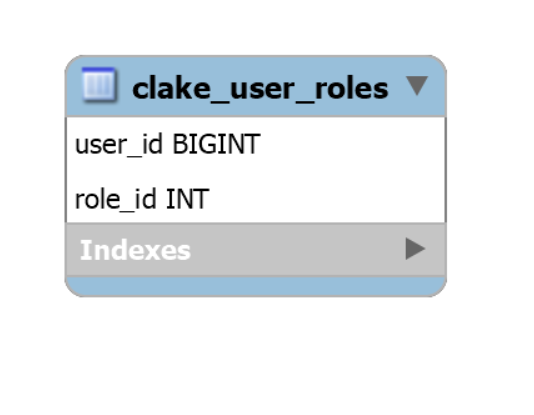
\includegraphics[width=0.3\textwidth]{images/DatabaseUserRoleDesign.PNG}
\end{table}
\begin{itemize}
    \item "clake\_user\_roles" is a table containing user and their associated role.
    \item This table connects with the "clake\_users" table and "clake\_roles" table with the Foreign Key: 'user\_id' and 'role\_id'. This is "many to many" relationship: Each "User" could have many roles. Each "Role" could have many users.  
\end{itemize}

\begin{table}[H]
  \centering
  \caption{Database Group Design}
  \label{tbl:dbGroup}
  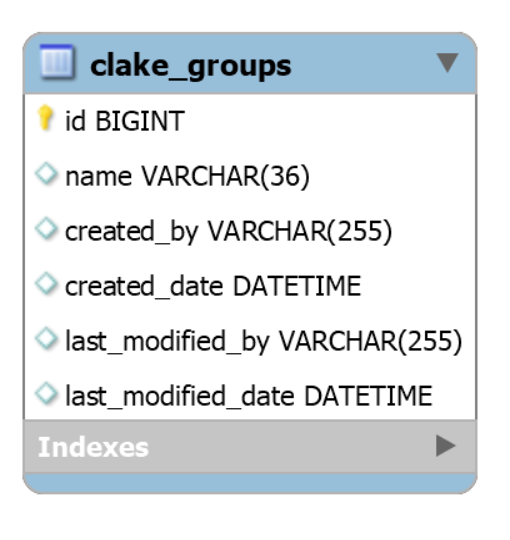
\includegraphics[width=0.3\textwidth]{images/DatabaseUserGroupDesign.PNG}
\end{table}
\begin{itemize}
    \item "clake\_groups" is the table that contains the information of groups, for example group name. 
    \item This table has "id" as Primary Key. Each group has an unique "id". 
    \item Group name must be unique from each other.
    \item This table is audit-able, by the field 'created\_by', 'created\_date', 'last\_modified\_by' and 'last\_modified\_date'. It will monitoring and recording of selected user database actions.
\end{itemize}

\begin{table}[H]
  \centering
  \caption{Database User Group Design}
  \label{tbl:dbUserGroup}
  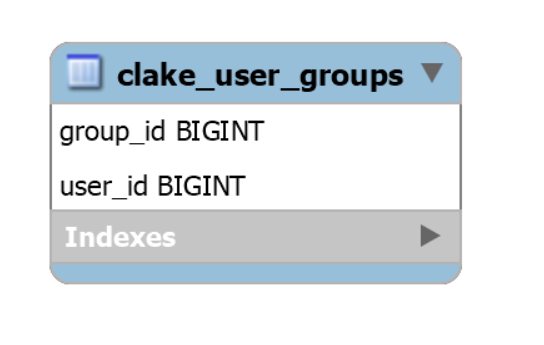
\includegraphics[width=0.3\textwidth]{images/DatabaseUserAGroupDesign.PNG}
\end{table}
\begin{itemize}
    \item "clake\_user\_groups" is a table containing user and their associated group.
    \item This table connects with the "clake\_users" table and "clake\_groups" table with the Foreign Key: 'user\_id' and 'group\_id'. This is "many to many" relationship: Each "User" could have many groups. Each "Group" could have many users.  
\end{itemize}

\begin{table}[H]
  \centering
  \caption{Database Refresh Token Design}
  \label{tbl:dbRefreshToken}
  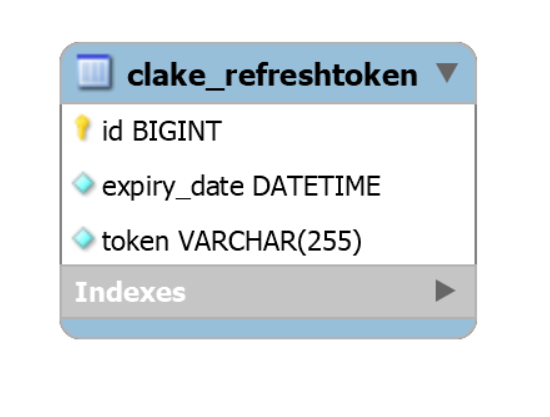
\includegraphics[width=0.3\textwidth]{images/DatabaseRefreshTokenDesign.PNG}
\end{table}
\begin{itemize}
    \item "clake\_refreshtoken" is the table that contains the refresh token information of an user.
    \item This will keep user logged in longer time with silent authentication because it has longer expiry date than the access token. 
    \item This table has "id" as Primary Key.
    \item This has one-to-one relationship with "User".
\end{itemize}

\begin{table}[H]
  \centering
  \caption{Database Folder Design}
  \label{tbl:dbFolder}
  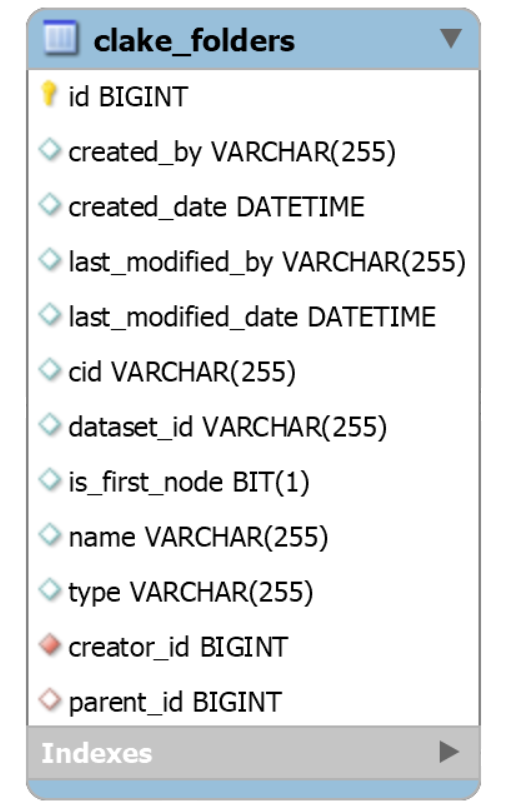
\includegraphics[width=0.3\textwidth]{images/DatabaseFolderDesign.PNG}
\end{table}
\begin{itemize}
    \item "clake\_folders" is the table that contains the information of folders.
    \item This table has "id" as Primary Key. Each folder has an unique "id". 
    \item This table connects with the "clake\_users" table with the Foreign Key 'creator\_id'. This is "many to one" relationship: Many "Folder" belongs to a "User". 
    \item The column 'parent\_id' is a foreign key that refers to the primary key column 'id' of the table itself. This is parent-child relationship, it needed to represent nested, hierarchical structures: A "Folder" can have one or many children folders below it. And vice-versa, a "Folder" can have one or many parent folders above it. There is no limit for the nested level.
    \item Noted that this table doesn't include 'source' and 'topics' fields because that metadata is stored in the ComLake Core. We use 'cid' and 'dataset\_id' as identifier to connect to the Core. 
    \item This table is audit-able, by the field 'created\_by', 'created\_date', 'last\_modified\_by' and 'last\_modified\_date'. It will monitoring and recording of selected user database actions.
\end{itemize}
\begin{table}[H]
  \centering
  \caption{Database File Design}
  \label{tbl:dbFile}
  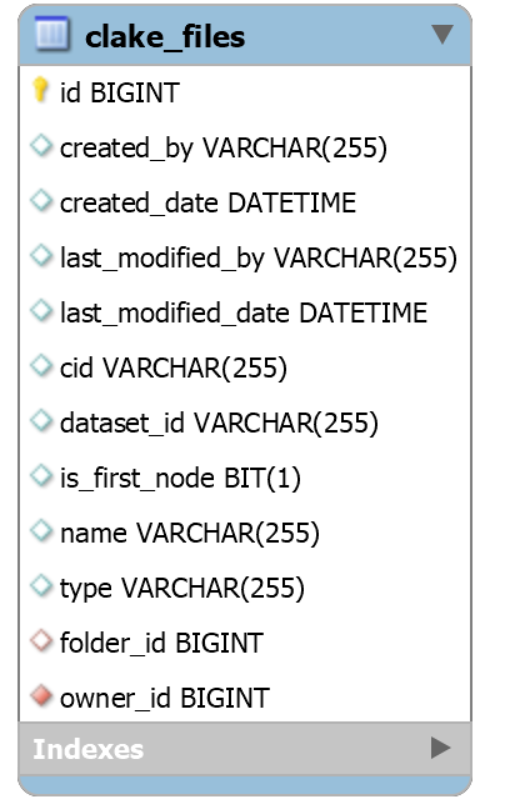
\includegraphics[width=0.3\textwidth]{images/DatabaseFileDesign.PNG}
\end{table}
\begin{itemize}
    \item "clake\_files" is the table that contains the information of files.
    \item This table has "id" as Primary Key. Each file has an unique "id". 
    \item This table connects with the "clake\_users" table with the Foreign Key 'owner\_id'. This is "many to one" relationship: Many "File" belongs to a "User".
    \item This table connects with the "clake\_folders" table with the Foreign Key 'folder\_id'. This is "many to one" relationship: Many "File" could be in a "Folder". 
    \item Noted that this table doesn't include 'source' and 'topics' fields because that metadata is stored in the ComLake Core. We use 'cid' and 'dataset\_id' as identifier to connect to the Core. 
    \item This table is audit-able, by the field 'created\_by', 'created\_date', 'last\_modified\_by' and 'last\_modified\_date'. It will monitoring and recording of selected user database actions.
\end{itemize}

\begin{table}[H]
  \centering
  \caption{Database ACL Class Design}
  \label{tbl:dbACL}
  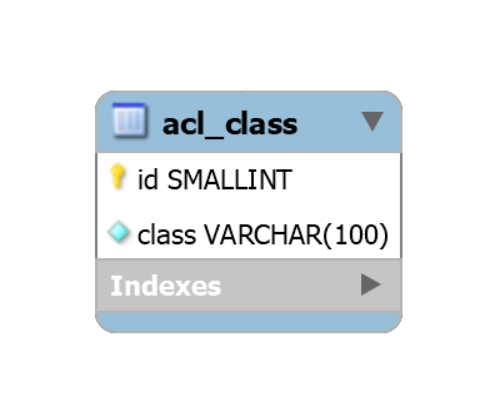
\includegraphics[width=0.3\textwidth]{images/DatabaseAclClassDesign.PNG}
\end{table}
\begin{itemize}
    \item "acl\_class" is the table that stores the class name of the domain object. 
    \item This table has "id" as Primary Key. Each file has an unique "id".
    \item In this system, we only have two classes that need to be secured: "File" and "Folder". So it will store two values: "com.ulake.api.models.File" and "com.ulake.api.models.Folder". 
\end{itemize}

\begin{table}[H]
  \centering
  \caption{Database ACL Sid Design}
  \label{tbl:dbACL}
  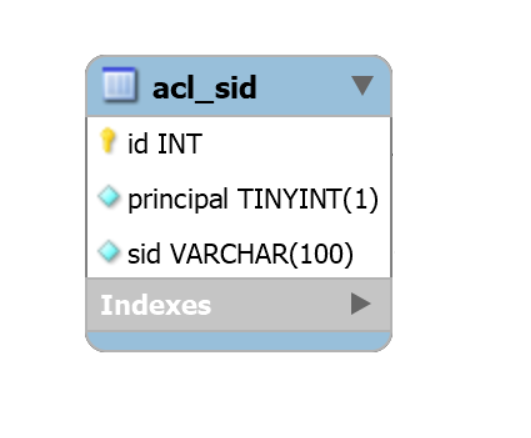
\includegraphics[width=0.3\textwidth]{images/DatabaseAclSidDesign.PNG}
\end{table}
\begin{itemize}
    \item "acl\_sid" is the table that allows us to universally identify any users, roles or groups in the system. 
    \item This table has "id" as Primary Key. Each file has an unique "id".
    \item The field 'sid' could be username of the user or role name like "ROLE\_ADMIN" or group name. SID stands for "Security Identity".
    \item The field 'principal' could be 0 or 1. It is a Boolean value indicate if the corresponding 'sid' is a principal (user) or an authority (role or group). 
\end{itemize}

\begin{table}[H]
  \centering
  \caption{Database ACL Object Identity Design}
  \label{tbl:dbACL}
  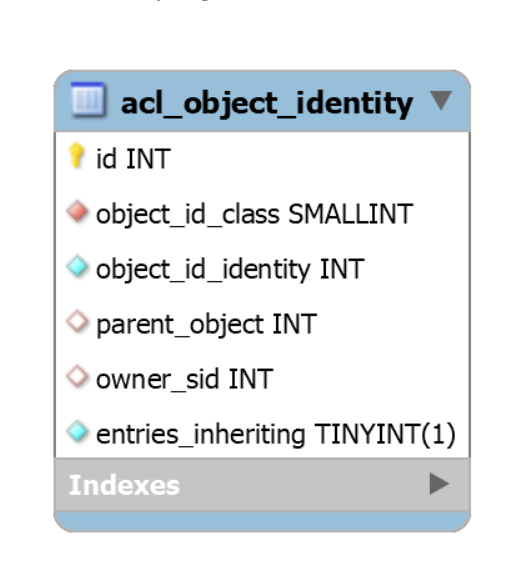
\includegraphics[width=0.3\textwidth]{images/DatabaseAclOIDesign.PNG}
\end{table}
\begin{itemize}
    \item "acl\_object\_identity" is the table that stores the information for each unique domain object (File or Folder). 
    \item This table has "id" as Primary Key. Each file has an unique "id".
    \item The field 'object\_id\_class' indicate if it is File or Folder.
    \item The field 'owner\_sid' links to "acl\_sid" table. It is the Id of the owner. 
\end{itemize}

\begin{table}[H]
  \centering
  \caption{Database ACL Entry}
  \label{tbl:dbACL}
  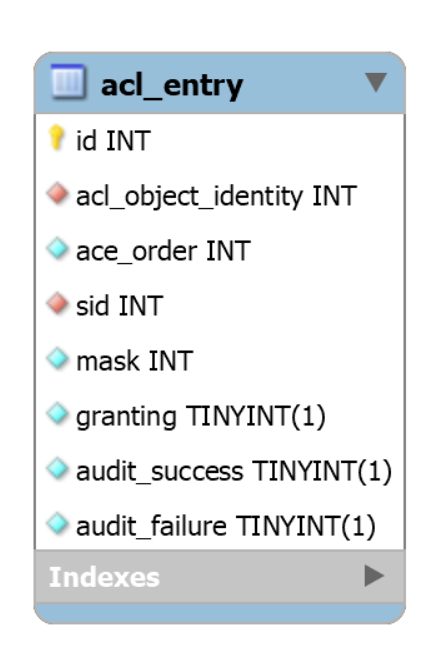
\includegraphics[width=0.3\textwidth]{images/DatabaseAclEntryDesign.PNG}
\end{table}
\begin{itemize}
    \item "acl\_entry" is the table that stores individual permission assigns to each SID on an Object Identity.
    \item This table has "id" as Primary Key. Each file has an unique "id".
    \item The field 'acl\_object\_identity' specify the object identity, links to "acl\_object\_identity" table. 
    \item The field 'ace\_order' is the order of current entry in the ACL entries list of corresponding Object Identity.
    \item The field 'sid' is the target SID which the permission is granted to or denied from, links to "acl\_sid" table.
\end{itemize}

\begin{table}[H]
  \centering
  \caption{Database ACL Design}
  \label{tbl:dbACL}
  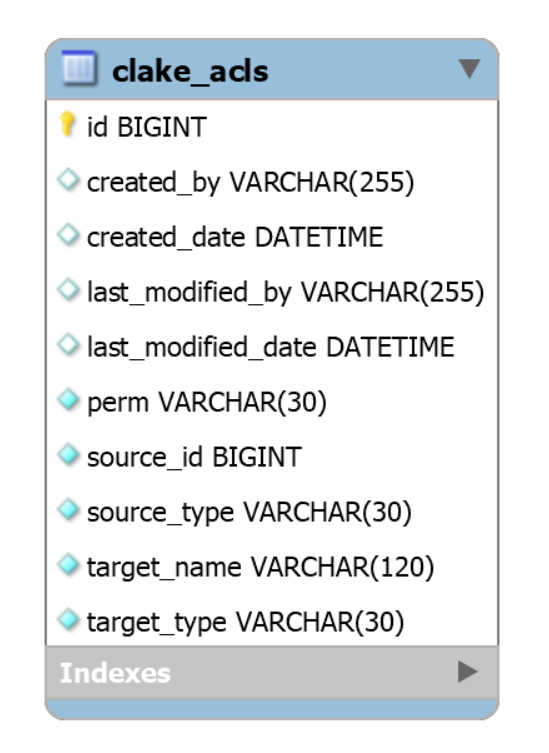
\includegraphics[width=0.3\textwidth]{images/DatabaseAclDesign.PNG}
\end{table}
\begin{itemize}
    \item "clake\_acls" is the table that mimics the table "acl\_entry" for easier interface.
    \item This table has "id" as Primary Key. Each file has an unique "id".
    \item The field 'source\_type' could be "File" or "Folder".
    \item The field 'target\_type' could be "User" or "Group". 
    \item The field 'perm' could be "Read" or "Write". 
    \item This table is audit-able, by the field 'created\_by', 'created\_date', 'last\_modified\_by' and 'last\_modified\_date'. It will monitoring and recording of selected user database actions.
\end{itemize}
\section{Use Cases Implementation}
\subsection{Login}
This use case describes how a user logs into the system. This user can be a Admin or a (Regular) User. When a user wants to login, the system requests the actor to enter username and password (Figure \ref{fig:login} in Appendices). Once the user enters the username and password, the system will check if the information is valid and logs the user in. Otherwise, the system displays and error message and asks the user to re-enter the information. 
\begin{figure}[H]
    \centering
    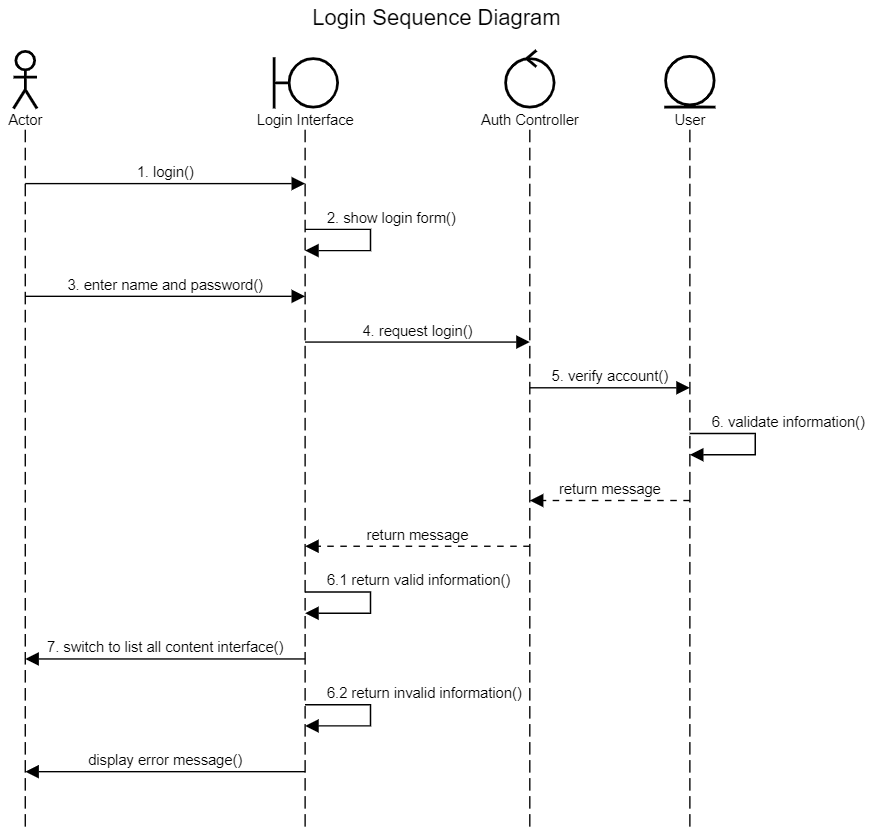
\includegraphics[width=1.0\textwidth]{images/LoginSequence.png}
    \caption{Login Sequence diagram}
    \label{fig:LoginSeq}
\end{figure}

\subsection{Register}
This use case describes how a user registers to the system. When a user wants to register into the system, the system will display a register interface and requests that the user enter first name, last name, email, username, and password (Figure \ref{fig:register} in Appendices). After the user enters the required information, the system checks if the entered email and username are unique from the table "comlake\_users" in Database. If unique, the system encrypts the password, saves the user information, assigns a unique id to the user, and redirects to the login interface. Otherwise, the system displays an error message and asks the user to re-enter the information.

\begin{figure}[H]
    \centering
    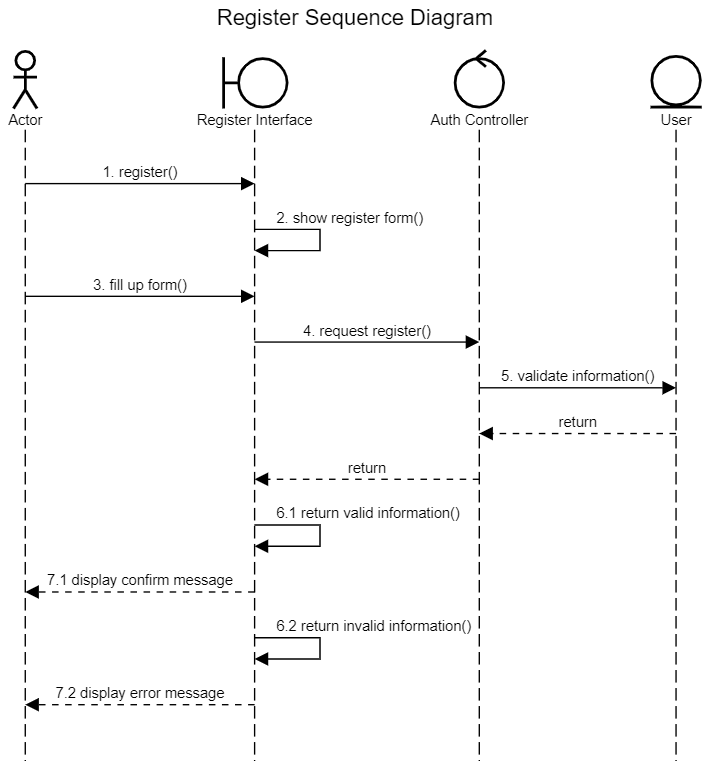
\includegraphics[width=1.0\textwidth]{images/RegisterSequence.png}
    \caption{Register Sequence diagram}
    \label{fig:RegisterSeq}
\end{figure}

\subsection{Manage Users}
This Use Case describes how an Admin can manage users.

\subsubsection{Manage Users - Basic flow}
When the Admin logged into the system, there will be a User tab if the Admin wishes to manage users. The system lists all of the users (Figure \ref{fig:adminAllUsers} in Appendices). The Admin can filter users with desired criteria, and the system will respond to a list of users according to the criteria. The Admin could choose to perform an action (create, edit, delete). If the Admin chooses to create a user, there will be a create user form (Figure \ref{fig:adminCreateUser} in Appendices). After the Admin enters the required information, the system checks if the entered email and username are unique from the table "comlake\_users" in Database. If unique, the system encrypts the password, saves the user information, assigns a unique id to the user, and redirects to the login interface. Otherwise, the system displays an error message and asks the Admin to re-enter the information. 
\begin{figure}[H]
    \centering
    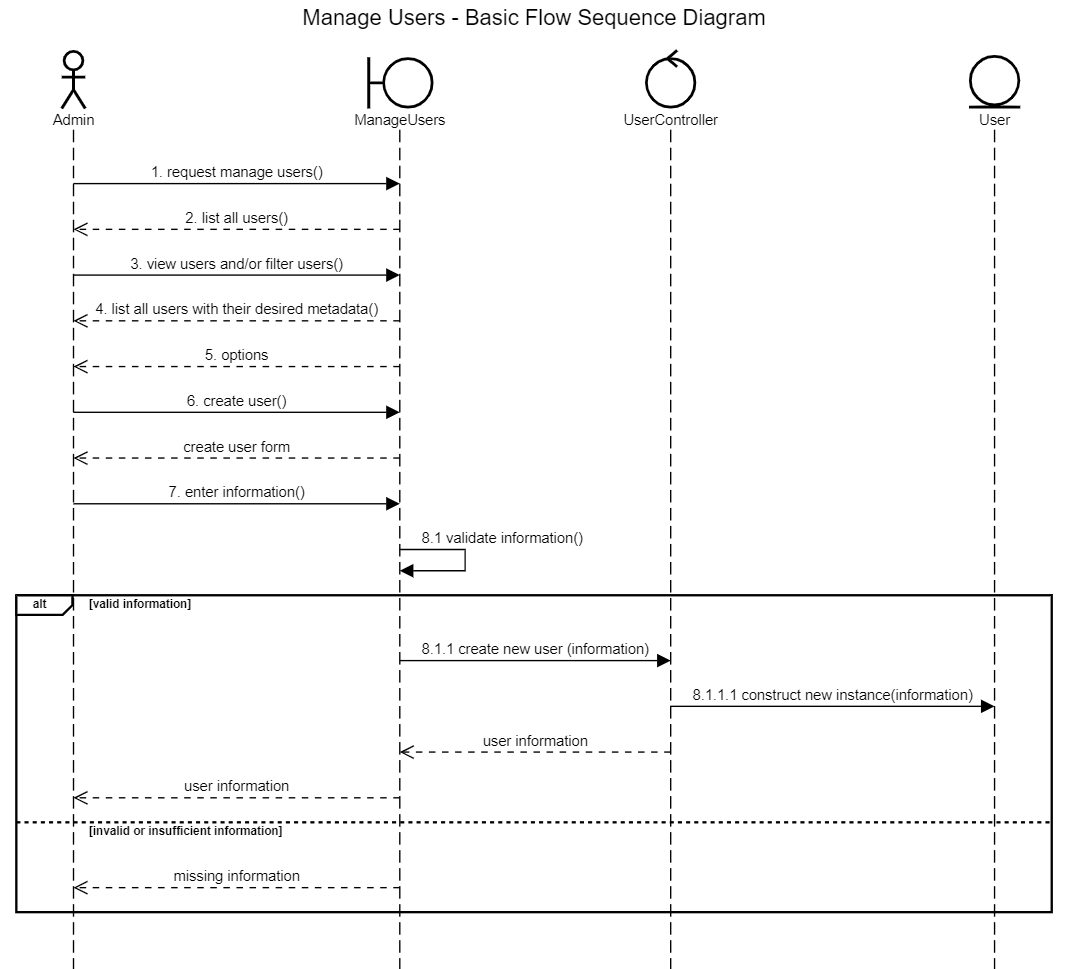
\includegraphics[width=1.0\textwidth]{images/Manage Users - Basic Flow Sequence Diagram.png}
    \caption{Manage Users - Basic Flow Sequence diagram}
    \label{fig:SeqUsersBasic}
\end{figure}

\subsubsection{Update User - Sub flow}
If the Admin wishes to edit a user by select the target user, the system will display an update user form (Figure \ref{fig:adminEditDeleteUser} in Appendices). After the Admin enters the updated information, the system will check if the user exists or not. If the user exists, the system will save the updated information of the user. If not, the system displays an error message. 

\begin{figure}[H]
    \centering
    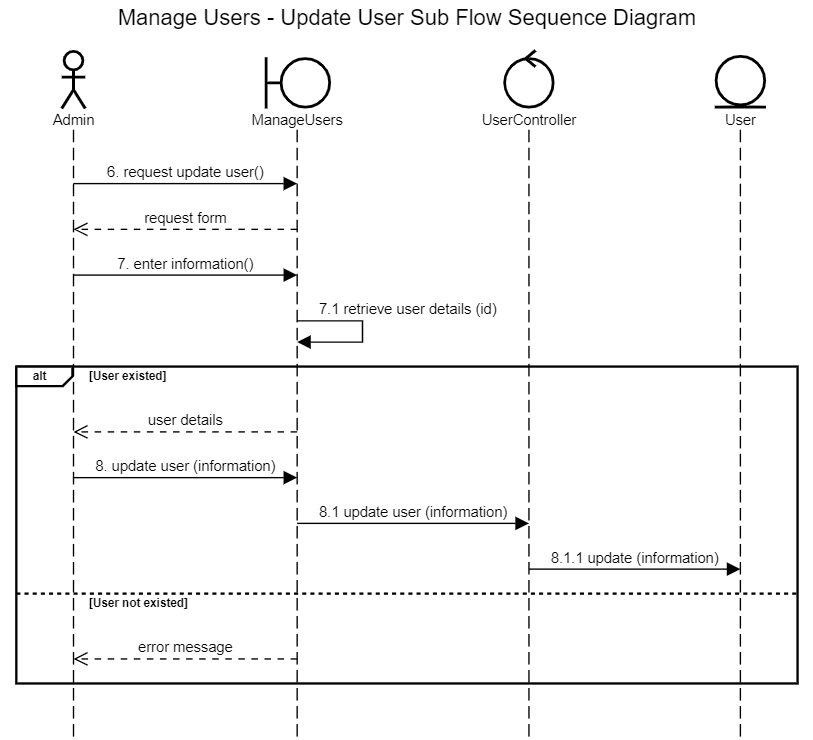
\includegraphics[width=1.0\textwidth]{images/Manage Users - Update User Sub Flow Sequence Diagram.png}
    \caption{Manage Users - Update User Sub Flow Sequence diagram}
    \label{fig:SeqUsersUpdate}
\end{figure}

\subsubsection{Delete User - Sub flow}
If the Admin wished to delete a user by selecting the target user, the system would display the full details of the user. When Admin clicks on the "Delete" button, the system will checks if the user exists or not. If the user exists, the system will remove the user. If not, the system displays an error message.
\begin{figure}[H]
    \centering
    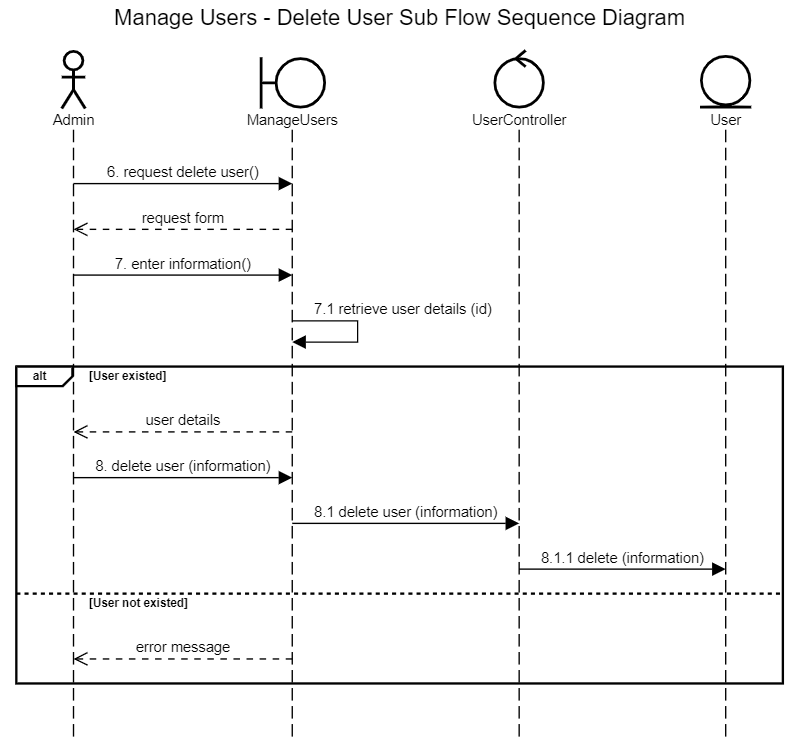
\includegraphics[width=1.0\textwidth]{images/Manage Users - Delete User Sub Flow Sequence Diagram.png}
    \caption{Manage Users - Delete User Sub Flow Sequence diagram}
    \label{fig:SeqUsersDelete}
\end{figure}

\subsection{Manage User Groups}
This Use Case describes how an Admin can manage user groups.
\subsubsection{Manage User Groups - Basic flow}
When the Admin logged into the system, there will be a User tab if the Admin wishes to manage user groups. The system lists all of the user groups (Figure \ref{fig:adminListAllGroups} in Appendices). The Admin can filter user groups with desired criteria, and the system will respond to a list of user groups according to the criteria. The Admin could choose to perform action (create, edit, delete). If the Admin choose to create group, there will be a create group form (Figure \ref{fig:adminCreateGroup} in Appendices). After the Admin enters the required information, the system checks if the entered name are unique from the table "comlake\_user\_groups" in Database. If unique, the system saves the group information, assigns a unique id to the group, and redirects to the login interface. Otherwise, the system displays an error message and asks the Admin to re-enter the information. 
\begin{figure}[H]
    \centering
    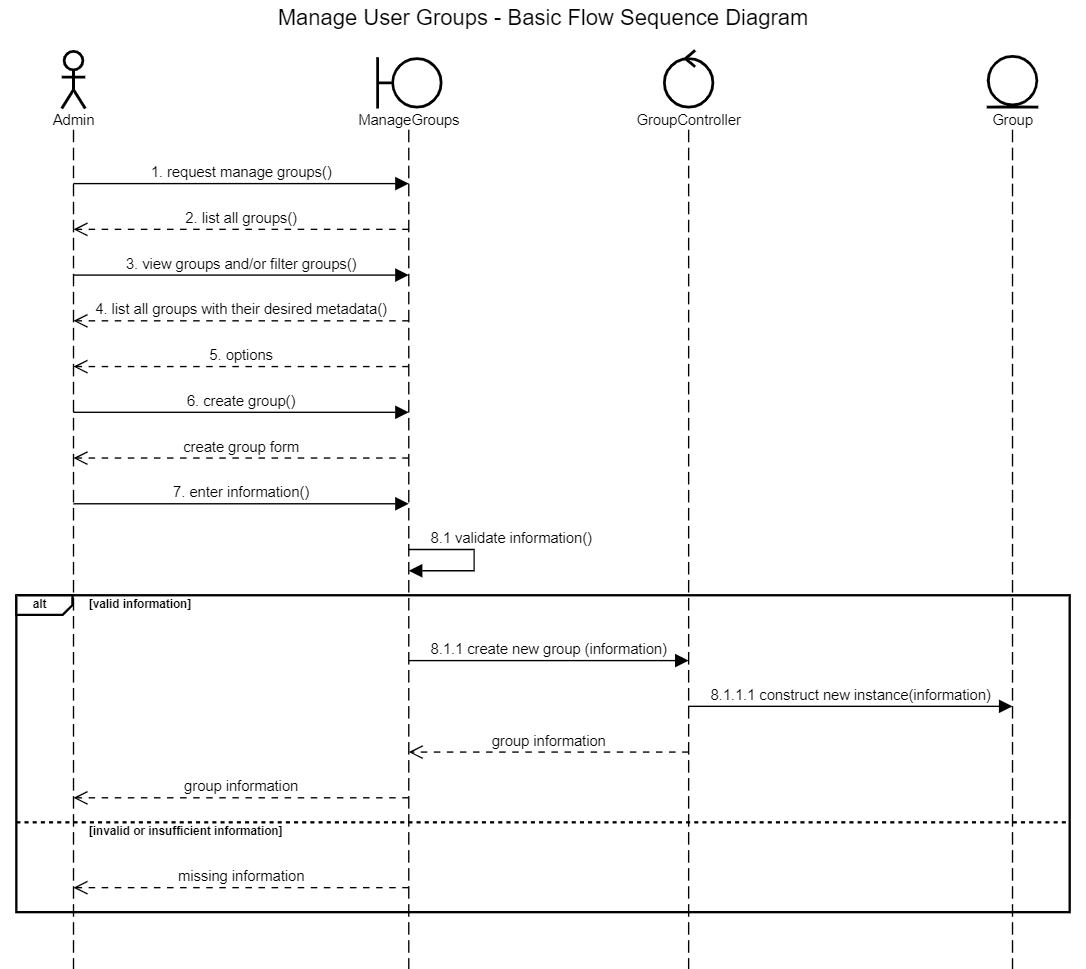
\includegraphics[width=1.0\textwidth]{images/Manage User Groups - Basic Flow Sequence Diagram.png}
    \caption{Manage Groups - Basic Flow Sequence diagram}
    \label{fig:SeqGroupsBasic}
\end{figure}
\subsubsection{Update Group - Sub flow}
If the Admin wishes to edit by selecting the target group, the system will display an update group[ form (Figure \ref{fig:adminUpdateGroup} in Appendices). After the Admin enters the updated information, the system will check if the group exists or not. If the group exists, the system will save the updated information of the group. If not, the system displays an error message. 
\begin{figure}[H]
    \centering
    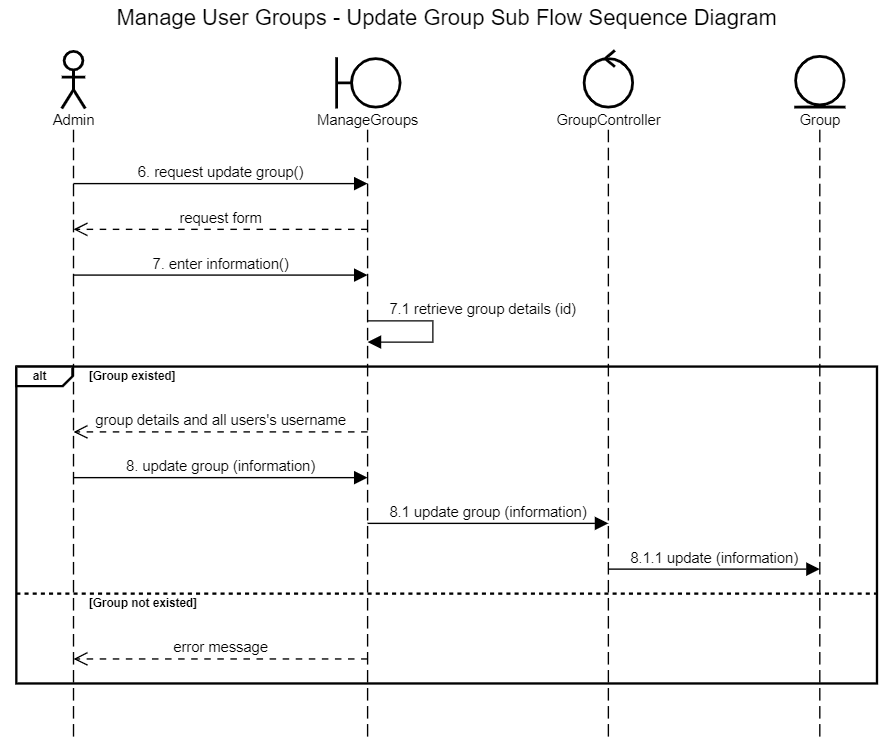
\includegraphics[width=1.0\textwidth]{images/Manage User Groups - Update Group Sub Flow Sequence Diagram.png}
    \caption{Manage User Groups - Update Group Sub Flow Sequence diagram}
    \label{fig:SeqGroupsUpdate}
\end{figure}
\subsubsection{Delete Group - Sub flow}
If the Admin wished to delete a group by selecting the target group, the system would display the full details of the group. When Admin clicks on the "Delete" button, the system will checks if the group exists or not. If the group exists, the system will remove the group. If not, the system displays an error message.
\begin{figure}[H]
    \centering
    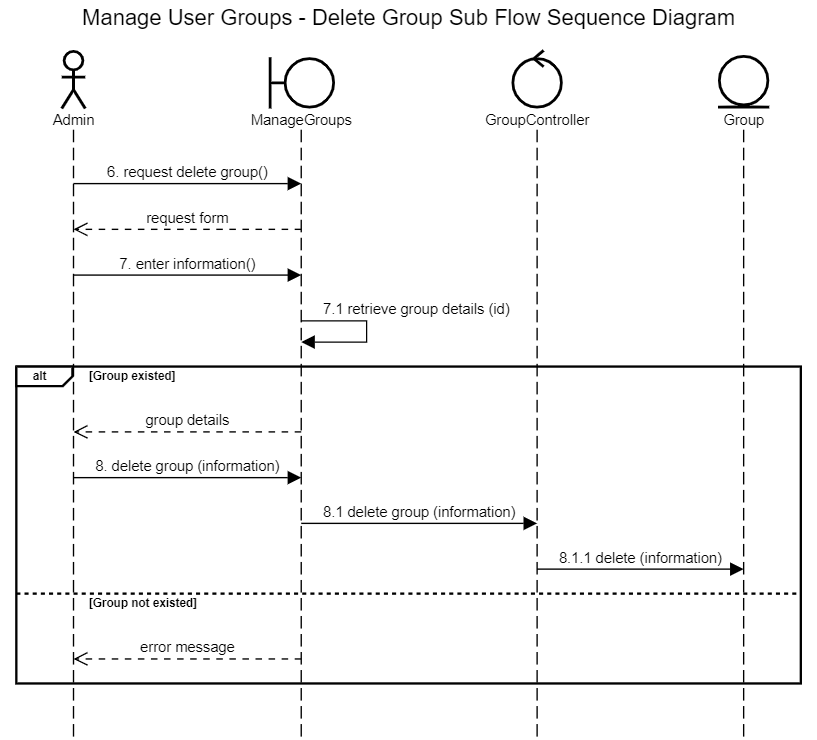
\includegraphics[width=1.0\textwidth]{images/Manage User Groups - Delete Group Sub Flow Sequence Diagram.png}
    \caption{Manage User Groups - Delete Group Sub Flow Sequence diagram}
    \label{fig:SeqGroupsDelete}
\end{figure}

\subsection{Manage Folders}
This Use Case describes how a User can manage folders.

\subsubsection{Manage Folders - Basic flow}
When the User logged into the system, the system lists all of the files and folders (Figure \ref{fig:listContent} in Appendices). The User can filter folders with desired criteria, and the system will respond to a list of folders. The User could choose to perform an action (create, edit, delete, move). If the User does not have permission to view a folder, that folder will not appear in the folder list. If the User chooses to create a folder, there will be a create folder form (Figure \ref{fig:createFolder} in Appendices). After the User enters all the required information, the system saves the folder information, assigns a unique id to the folder, and redirects to the files and folders interface. Otherwise, the system displays an error message and asks the User to re-enter the information. 

\begin{figure}[H]
    \centering
    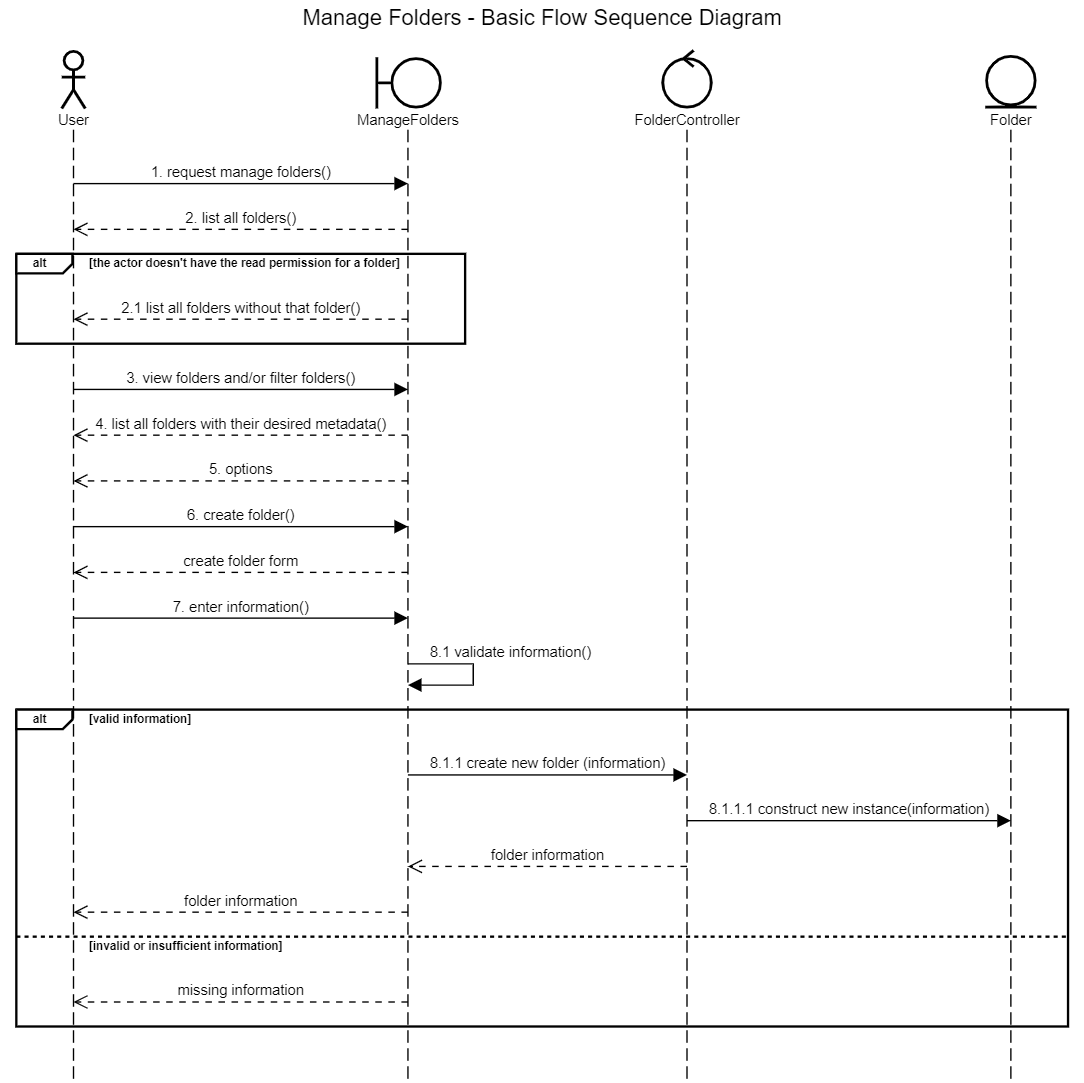
\includegraphics[width=1.0\textwidth]{images/Manage Folders - Basic Flow Sequence Diagram.png}
    \caption{Manage Folders - Basic Flow Sequence diagram}
    \label{fig:SeqFoldersBasic}
\end{figure}

\subsubsection{Update Folder - Sub flow}
If the User wishes to edit a folder by select the target folder, the system will check if the User have the right to write the folder. If the User does not have a write permission to a folder, the system will display en error message. Else, the system will display an update folder f\ref{fig:editFolder} in Appendices). After the User enters the updated information, the system will check if the folder exists or not. If the folder exists, the system will save the updated information of the folder. If not, the system displays an error message. 

\begin{figure}[H]
    \centering
    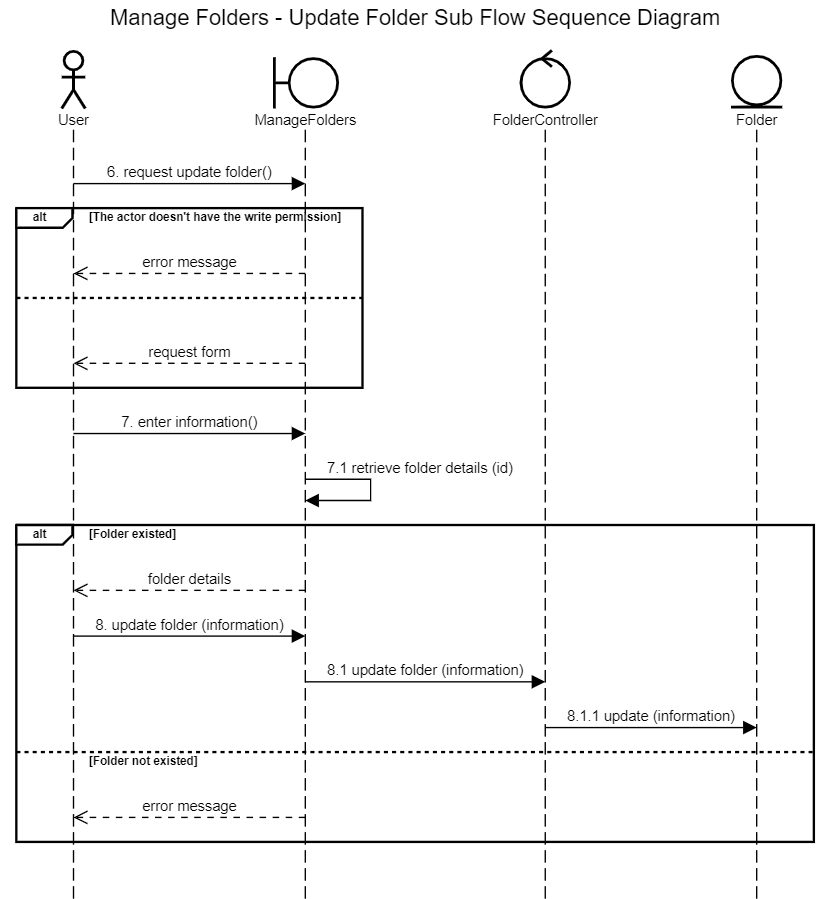
\includegraphics[width=1.0\textwidth]{images/Manage Folders - Update Folder Sub Flow Sequence Diagram.png}
    \caption{Manage Folders - Update Folder Sub Flow Sequence diagram}
    \label{fig:SeqFoldersUpdate}
\end{figure}

\subsubsection{Delete Folder - Sub flow}
If the User wished to delete a folder by selecting the target folder, the system will check if the User have the right to write the folder. If the User does not have a write permission to a folder, the system will display en error message. Else, the system would display the full details of the folder. When User clicks on the "Delete" button, the system will checks if the folder exists or not. If the folder exists, the system will remove the folder. If not, the system displays an error message.
\begin{figure}[H]
    \centering
    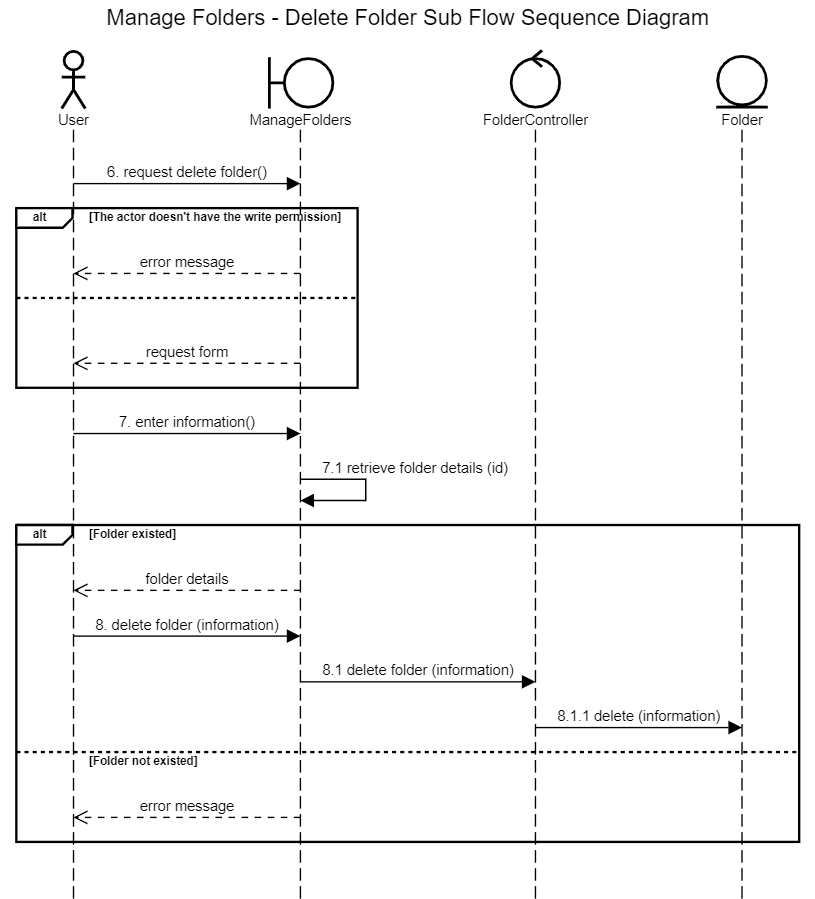
\includegraphics[width=1.0\textwidth]{images/Manage Folders - Delete Folder Sub Flow Sequence Diagram.png}
    \caption{Manage Folders - Delete Folder Sub Flow Sequence diagram}
    \label{fig:SeqFoldersDelete}
\end{figure}
\subsubsection{Move a Sub-folder a Folder - Sub flow}
If the User wishes to move a folder, the system will check if the User have the right to write the folder. If the User does not have a write permission to a folder, the system will display en error message. Else, the system will display a move folder form (Figure \ref{fig:moveContent}). The User will select a folder as source and enter the targeted folder and the destination folder. The system will move the targeted folder accordingly.  
\begin{figure}[H]
    \centering
    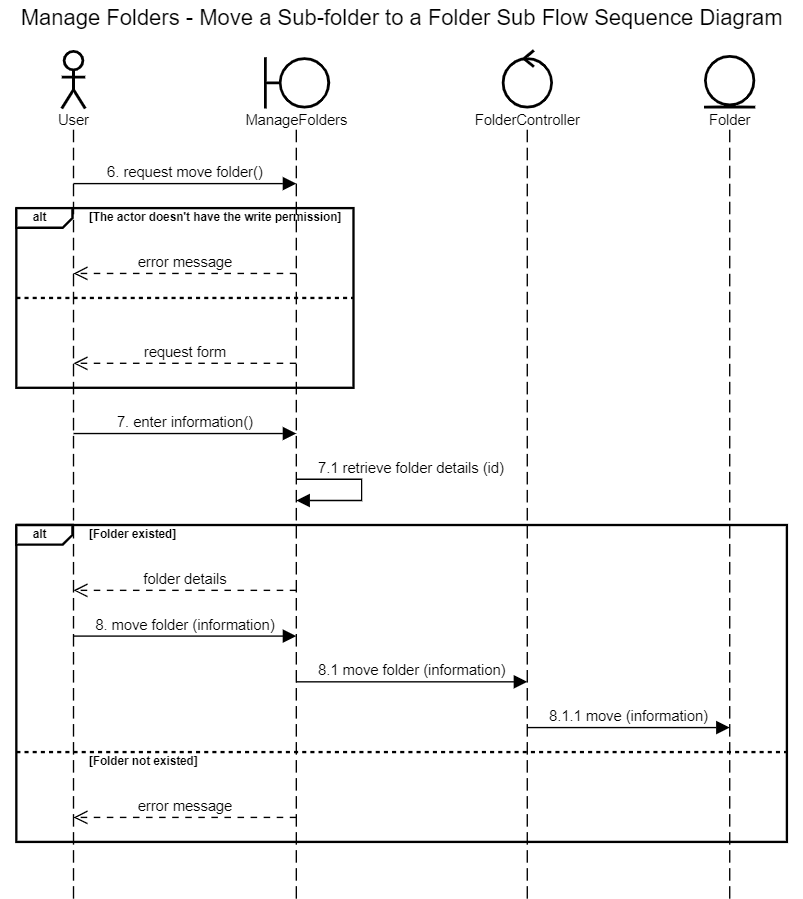
\includegraphics[width=1.0\textwidth]{images/Manage Folders - Move a Sub-folder to a Folder Sub Flow Sequence Diagram.png}
    \caption{Manage Folders - Move a Sub-folder to a Folder Sub Flow Sequence diagram}
    \label{fig:SeqFoldersMove}
\end{figure}

\subsection{Manage Files}
This Use Case describes how a User can manage files.
\subsubsection{Manage Files - Basic flow}
When the User logged into the system, the system lists all of the files and folders (Figure \ref{fig:listContent} in Appendices). The User can filter files with desired criteria, and the system will respond to a list of files. If the User does not have permission to view a file, that file will not appear in the file list. The User could choose to perform an action (upload, edit, delete, move, download). If the User chooses to upload, there will be an upload file form (Figure \ref{fig:uploadFile} in Appendices). After the User enters all the required information, the system saves the file information, assigns a unique id to the file, and redirects to the files and folders interface. Otherwise, the system displays an error message and asks the User to re-enter the information. 
\begin{figure}[H]
    \centering
    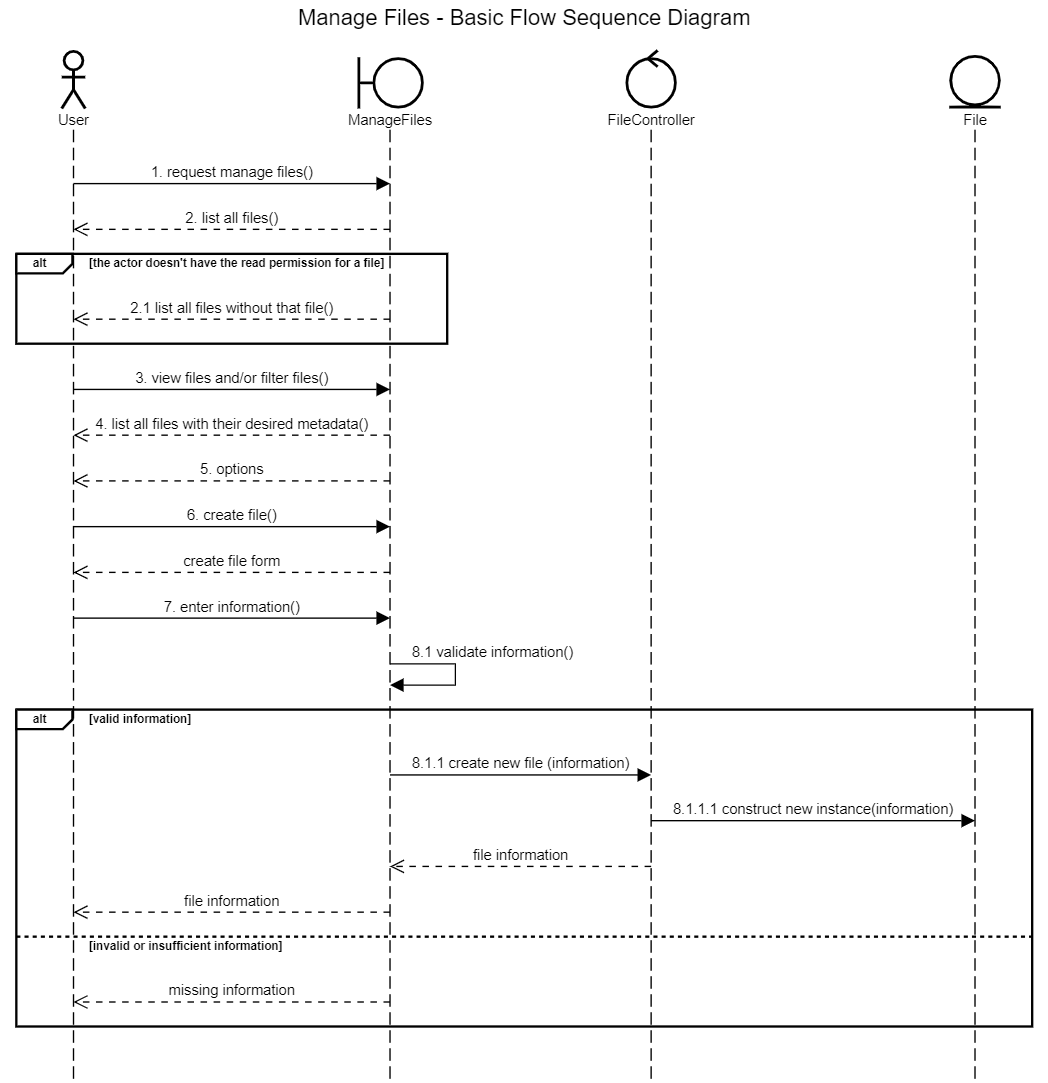
\includegraphics[width=1.0\textwidth]{images/Manage Files - Basic Flow Sequence Diagram.png}
    \caption{Manage Files - Basic Flow Sequence diagram}
    \label{fig:SeqFilesBasic}
\end{figure}
\subsubsection{Update File - Sub flow}
If the User wishes to edit a file by select the target file, the system will check if the User have the right to write the file. If the User does not have a write permission to a file, the system will displays en error message. Else, the system will display an update file f\ref{fig:editFile} in Appendices). After the User enters the updated information, the system will check if the file exists or not. If the file exists, the system will save the updated information of the file. If not, the system displays an error message. 

\begin{figure}[H]
    \centering
    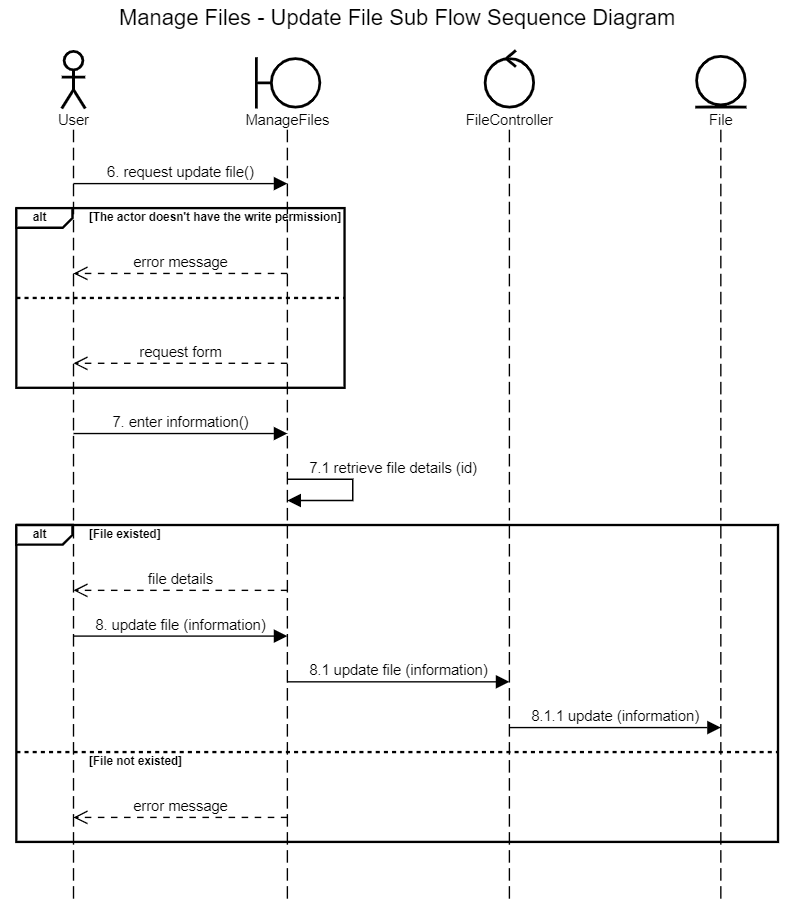
\includegraphics[width=1.0\textwidth]{images/Manage Files - Update File Sub Flow Sequence Diagram.png}
    \caption{Manage Files - Update File Sub Flow Sequence diagram}
    \label{fig:SeqFilesUpdate}
\end{figure}
\subsubsection{Delete File - Sub flow}
If the User wished to delete a file by selecting the target file, the system will check if the User have the right to write the file. If the User does not have a write permission to a file, the system would display an error message. Else, the system would display the full details of the file. When User clicks on the "Delete" button, the system will checks if the file exists or not. If the file exists, the system will remove the file. If not, the system displays an error message.
\begin{figure}[H]
    \centering
    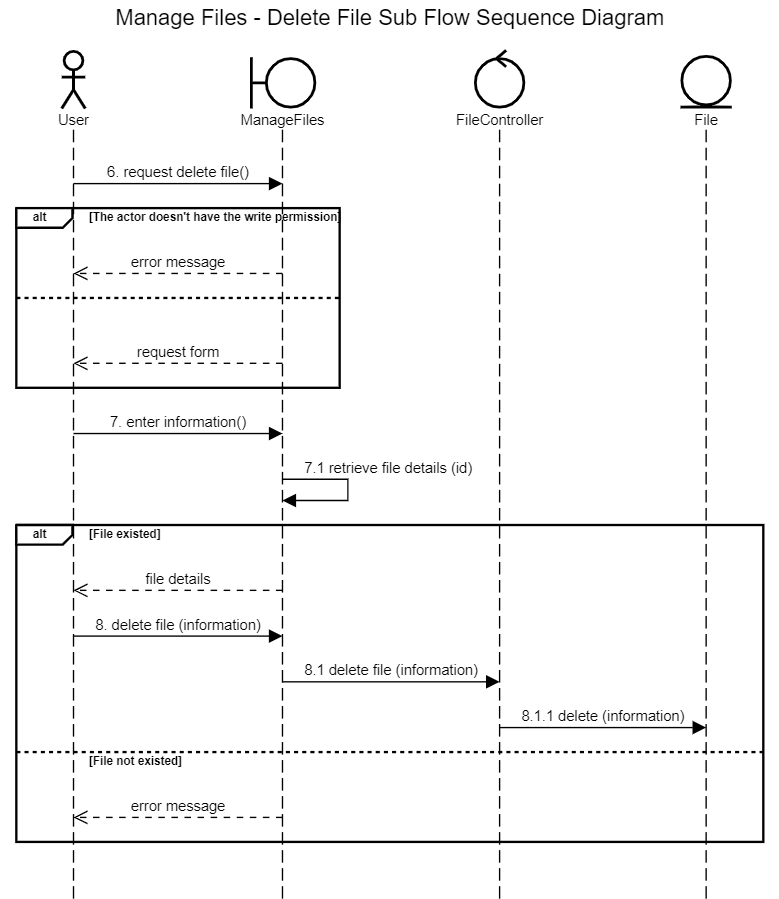
\includegraphics[width=1.0\textwidth]{images/Manage Files - Delete File Sub Flow Sequence Diagram.png}
    \caption{Manage Files - Delete File Sub Flow Sequence diagram}
    \label{fig:SeqFilesDelete}
\end{figure}
\subsubsection{Move a File a Folder - Sub flow}
If the User wishes to move a file, the system will check if the User have the right to write the file. If the User does not have a write permission to a file, the system will display an error message. Else, the system will display a move file form (Figure \ref{fig:moveContent}). The User will select a file as source and enter the targeted folder and the destination folder. The system will move the targeted file accordingly.  
\begin{figure}[H]
    \centering
    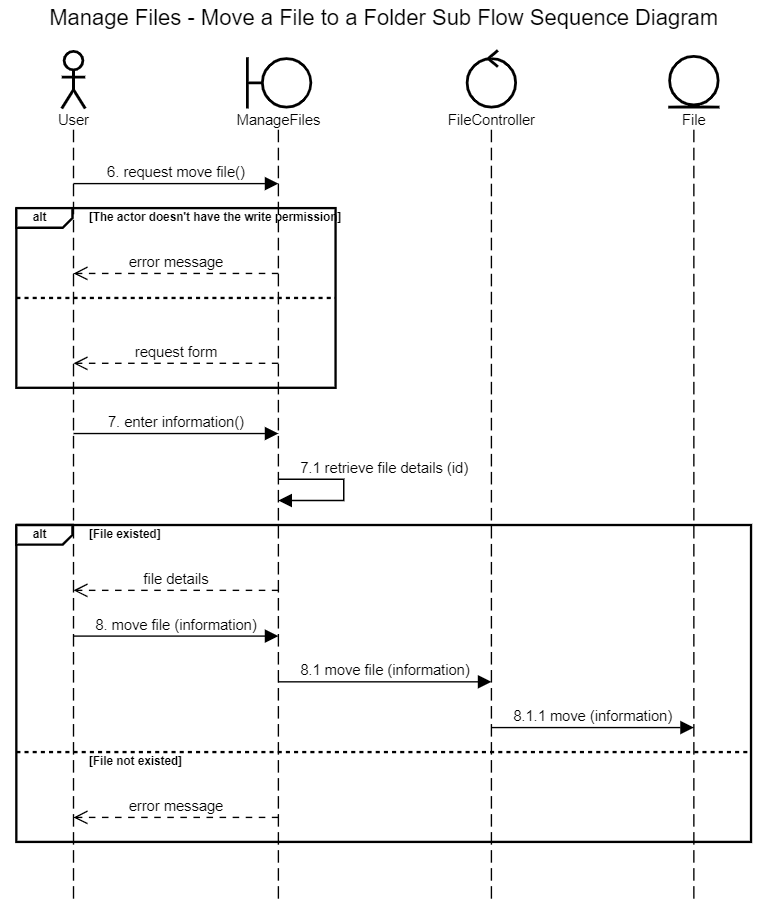
\includegraphics[width=1.0\textwidth]{images/Manage Files - Move a File to a Folder Sub Flow Sequence Diagram.png}
    \caption{Manage Files - Move a File to a Folder Sub Flow Sequence diagram}
    \label{fig:SeqFilesMove}
\end{figure}
\subsubsection{Download File - Sub flow}
If the User wishes to download a file, the system will check if the User have the right to view the file. If the User does not have a view permission to a file, the system will display an error message. Else, the system will process to return the file data for the user.  
\begin{figure}[H]
    \centering
    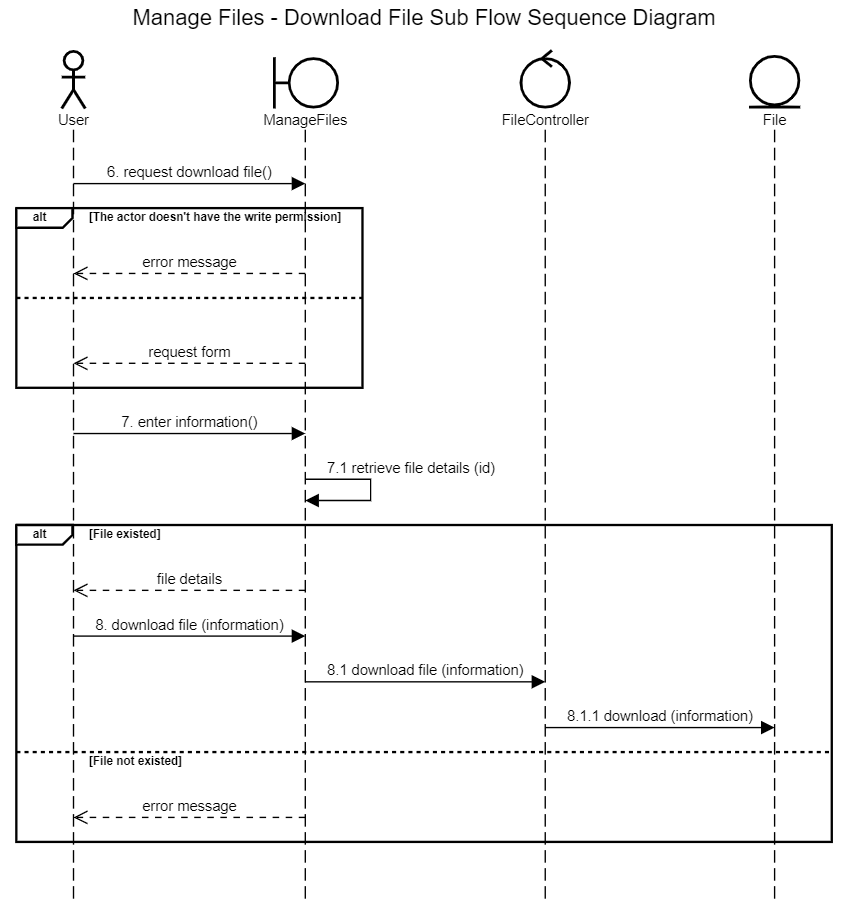
\includegraphics[width=1.0\textwidth]{images/Manage Files - Download File Sub Flow Sequence Diagram.png}
    \caption{Manage Files - Download File Sub Flow Sequence diagram}
    \label{fig:SeqFilesDownload}
\end{figure}

\subsection{Manage ACLs}
This Use Case describes how a User can manage ACLs permission.
\subsubsection{Manage ACLs - Basic flow}
In the selected file or folder, the User wishes to manage ACL permissions (grant or delete). If the User chooses to grant, there will be an grant ACL form (Figure \ref{fig:viewFile} and Figure \ref{fig:viewFolder} in Appendices). After the User enters all the required information, the system saves the ACL information, assigns a unique id to the ACL. Otherwise, the system displays an error message and asks the User to re-enter the information. 
\begin{figure}[H]
    \centering
    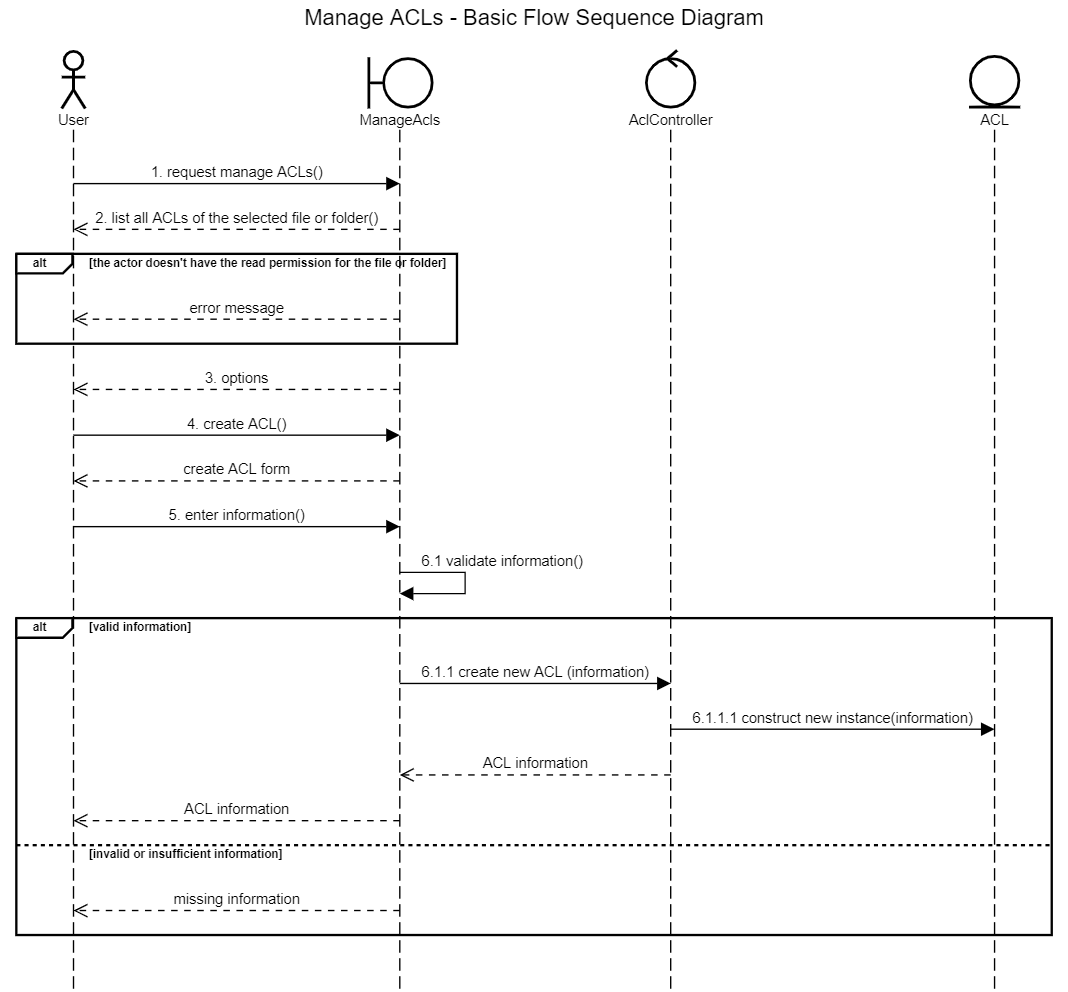
\includegraphics[width=1.0\textwidth]{images/Manage ACLs - Basic Flow Sequence Diagram.png}
    \caption{Manage ACLs - Basic Flow Sequence diagram}
    \label{fig:SeqACLsBasic}
\end{figure}
\subsubsection{Delete ACL - Sub flow}
If the User wished to delete a ACL by selecting the target ACL, the system will check if the User have the right to write the file or folder. If the User does not have a write permission, the system would display an error message. Else, the system would display the full details of the file or folder. When User clicks on the "Delete" button, the system will checks if the ACL exists or not. If the ACL exists, the system will remove the ACL. If not, the system displays an error message.
\begin{figure}[H]
    \centering
    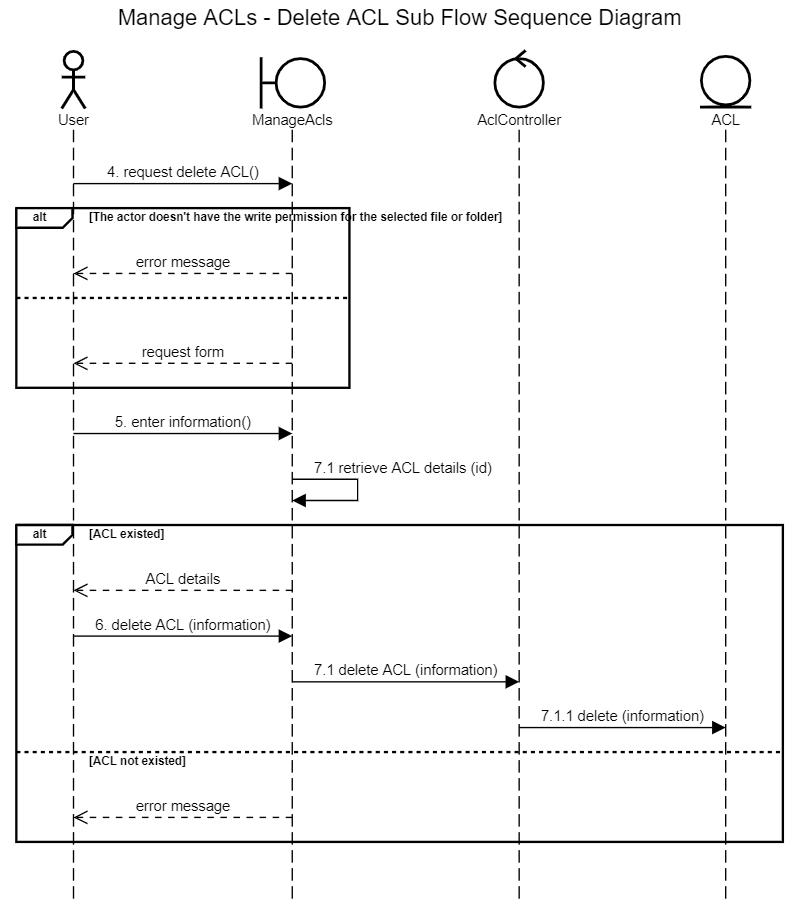
\includegraphics[width=1.0\textwidth]{images/Manage ACLs - Delete ACL Sub Flow Sequence Diagram.png}
    \caption{Manage ACLs - Delete ACL Sub Flow Sequence diagram}
    \label{fig:SeqACLsDelete}
\end{figure}

\section{Tools and Techniques}
\subsection{SQL}
With so much data and business relationships in our system, selecting a suitable database to manage it is critical. SQL is the clear choice because the project needs a close consistency between the data with high transactions and data security. While NoSQL has unstable schemas and is not fit for complex queries. Therefore, the best solution for our system is using SQL Database.\cite{mysql}

\subsection{Spring Boot}
Spring Boot is based on the Spring framework and has several dependencies that can be integrated into a Spring application. Spring Kafka, Spring LDAP, Spring Web Services, and Spring Security are some examples. \cite{spring}

Spring Boot uses Java, which is one of the most popular programming languages in the world. It reduces development time, increases the development team's overall productivity, and helps autoconfigure all components for a production-grade Spring application.

The dependency injection element of the Spring framework focuses on offering flexibility. It facilitates the injection of required dependencies and the development of a loosely linked application. It is a lightweight framework that is compatible with many middleware services.

\subsection{ReactJS}
React.js is an open-source JavaScript package to create single-page apps' user interfaces. For web and mobile apps, it is used to manage the view layer. We can also make reusable UI components with React. \cite{reactjs}
 
React allows developers to create large web applications that can change data without reloading the page. The primary purpose of React is to be fast, scalable, and straightforward. It works only on user interfaces in the application. This corresponds to the view in the MVC template. It can be used with other JavaScript libraries or frameworks, such as Angular JS in MVC.

There are so many open-source platforms for making front-end web application development more accessible, like Angular. React has some benefits over other competitive technologies or frameworks. The component-based approach, well-defined lifecycle, and plain JavaScript make React very simple to learn, build a professional web (and mobile applications), and support it. React uses a special syntax called JSX, which allows us to mix HTML with JavaScript. It has a better learning curve than Angular because Angular is a 'Domain-specific Language'. React only requires basic knowledge of CSS and HTML.

For this project, according to the condition and the requirement of the system environment, React is a great choice compared to others. 

\subsection{Axios}
Axios is a popular, promise-based HTTP client \cite{axios} that sports an easy-to-use API and can be used in both the browser and Node.js.

One of the most common activities a client-side JavaScript application will have to perform is making HTTP requests to fetch or save data. Third-party libraries have long been a popular approach to deal with more verbose browser APIs while abstracting away any variations across browsers.

Axios can be used in both the browser and Node.js compared with Fetch API built in many modern browsers. One such difference is in how the two libraries treat HTTP error codes \cite{http}. When using Fetch, if the server returns a 4xx or 5xx series error, the catch() callback will not be triggered, and it is down to the developer to check the response status code to determine if the request was successful. On the other hand, Axios will reject the request promise if one of these status codes is returned.

One distinction that may prove to be a deal-breaker for some is status updates on uploads and downloads. We may register callback functions for onUploadProgress and onDownloadProgress to display the percentage completion in the app's UI because Axios is built on top of the older XHR API. Fetch cannot currently do so. Therefore, the best choice is using Axios.

\subsection{Material-UI}
Material-UI is based on Google's Material Design guidelines. Like other design systems, Material Design was intended to provide a uniform user experience across various devices, platforms, and input methods. Google adopted Material Design to ensure that users had a uniform user experience regardless of how they accessed their products. Apple embraced flat design principles as their standard. \cite{material}

Material-UI is the world's most popular React UI framework. It provides a strong foundation for building dynamic UIs. It is blazing fast. It uses JSS at its core – a high performance JavaScript to CSS compiler which works at runtime and server-side, with less than 15 KB gzipped; and no bundle size increase if used alongside Material-UI.

\subsection{Swagger}
API Documentation is needed because the application is connected to many other services. It will improve user adaption, save support time and costs, and easier maintenance.

Swagger with API description formats like the OpenAPI/Swagger Specification is an excellent choice for that purpose. It has automated the documentation process, making it easier for teams to generate and maintain them. \cite{swagger}

\subsection{JWT (JSON Web Token)}
JWT is now widely used for authentication and data exchange. The Server encodes data into a JSON Web Token and transmits it to the Client instead of starting a Session (Session-based Authentication). After the Client saves the JWT, it should be appended to every request from the Client to protected routes or resources (commonly at header). The Server will validate the JWT, and the response will be returned.

Compared to Session-based Authentication, which requires the storage of the session on a cookie, JWT (Token-based Authentication) has the substantial advantage of storing the token on the client-side: Local Storage for browsers, Keychain for iOS, and SharedPreferences for Android... As a result, we will not need to create a separate backend project for Native Apps or a separate Authentication module for Native App users. 

For that, using JWT is ideal for this project.

\subsection{RBAC and ACL Authorization}
We developed the authentication from JWT, which establishes the principal's identity. After then, authorization is required, which determines what the principal is permitted to do. We start with role-based authorization (RBAC), which involves assigning roles to specific users and then utilizing those roles to define what they may see and do, ideally through related permissions. Role Admin and Role User are two types of roles. 

When we have to maintain predicates on principals regarding specific targets, the problem occurs. When we discuss the data lake, we want to make it so that only the file owner and the admin may update a file after it has been posted and that no one else can do so without authorization. "Can User1 edit files in general?" is a question that role-based permission helps us answer. ACL-based authorization (Access Control List) is more fine-grained, requiring the management of relationships between actors and targets to answer the question, "Can User1 edit file 10?". \cite{authorization}

We implement ACL Authorization Model with the help of Spring Security's ACL module. 

\chapter{Results and Discussion}
\label{chap:results}
\section{Result}
After three months of development, the APIs and Dashboard for Data Lake has basically been completed, meeting the initial criteria. To be more specific, a website has been designed with the following functions:
\begin{itemize}
    \item \textbf{Register and Login}: Allows users to create an account and log in using the registered account based on username and a real email.
    \item \textbf{Manage Users}: Allow Admin to read, create, edit, and delete information about users.
    \item \textbf{Manage User Groups}: Allow Admin to read, create, edit, and delete information about groups.
    \item \textbf{Manage Folders and Manage Files}: Authorized users are allowed to read, create, edit, and delete information about files and folders. To increase productivity, users can filter them by custom criteria.
    \item \textbf{Manage ACLs}: Authorized users are allowed to grant permission for other users on the files or folders they selected.
\end{itemize}

\subsection{API}
These are all the endpoints for the API we have been building: 
\begin{longtable}{|p{2cm}|p{5cm}|p{5cm}|}
\caption{All API Endpoints}
\label{table:APIendpoints} \\

\hline \multicolumn{1}{|c|}{\textbf{Methods}} & \multicolumn{1}{c|}{\textbf{URLs}} & \multicolumn{1}{c|}{\textbf{Action}} \\ \hline 
\endfirsthead
  \hline 
POST & /api/auth/signup & Signup new account\\ \hline
POST & /api/auth/signin & Login an account\\ \hline
POST & /api/auth/refresh-token & Get access token from refresh token \\ \hline
GET & /api/auth/logout & Logout current user\\ \hline
GET & /api/users/check\_email & Check if Email is available to use \\ \hline
GET &
/api/users/my-profile &
Get the logged in's user profile \\ \hline

GET &
/api/users/\{id\} &
Get user by ID \\ \hline

PUT &
/api/users/\{id\} &
Update user by ID \\ \hline

DELETE &
/api/users/\{id\} &
Delete user by ID \\ \hline

GET &
/api/users/check\_username &
Check if Username is available to use \\ \hline

GET &
/api/users/find/{username} &
Get user by user name \\ \hline

GET &
/api/users &
Get a list of all users in the system \\ \hline

GET &
/api/groups/\{id\} &
Get a group by ID \\ \hline

DELETE &
/api/groups/\{id\} &
Delete a group \\ \hline

PUT &
/api/groups/\{groupId\}/users/ \newline\{username\} &
Add a user to a group \\ \hline

GET &
/api/groups/find/\{name\} &
Get a group by name \\ \hline

GET &
/api/groups &
Get all groups \\ \hline

POST &
/api/groups &
Add an user group \\ \hline

GET &
/api/find/name/\{name\} &
Find all files and folders by name containing \\ \hline

GET &
/api/find/topics &
Get files and folders by topics \\ \hline

GET &
/api/folders/ls/\{folderId\} &
List all files and subfolders inside the folder by ID \\ \hline

GET &
/api/content &
Get all first node files and folders \\ \hline

GET & 
/api/folders &
Get all folders \\ \hline

POST & 
/api/folders &
Add a folder \\ \hline

GET & 
/api/folders/\{id\} &
Get a folder by ID \\ \hline

PUT & 
/api/folders/\{id\} &
Update a folder by ID \\ \hline

DELETE & 
/api/folders/\{id\} &
Delete a folder \\ \hline

GET & 
/api/folders/content/\{id\} &
Get a list of content inside folder by ID \\ \hline

PUT & 
/api/folders/\{folderId\}/\newline subfolders/\{subfolderId\} &
Add a subfolder to folder \\ \hline

PUT & 
/api/folders/\{folderId\}/files/\newline\{fileId\} &
Add a file to a folder \\ \hline

GET &
/api/files/data/\{id\} &
Get File Data \\ \hline

GET &
/api/files/\{id\} &
Get a file by ID \\ \hline

PUT &
/api/files/\{id\} &
Update a file by ID \\ \hline

DELETE &
/api/files/\{id\} &
Delete a file by ID \\ \hline

GET &
/api/folder/\{folderId\}/files &
Get All Files by Folder Id \\ \hline

GET &
/api/files &
Get all files \\ \hline

POST & 
/api/files &
Upload a file \\ \hline

PUT &
/api/acl/file/user &
Grant File Permission For User \\ \hline

DELETE &
/api/acl/file/user &
Remove a File Permission For User \\ \hline

GET &
/api/acl/perm &
Get All Permissions \\ \hline

PUT &
/api/acl/folder/user &
Grant Folder Permission For User \\ \hline

DELETE &
/api/acl/folder/user &
Remove a File Permission For User \\ \hline

PUT &
/api/acl/file/group &
Grant File Permission For Group \\ \hline

DELETE &
/api/acl/file/group &
Remove a File Permission For Group \\ \hline

PUT &
/api/acl/folder/group &
Grant Folder Permission For Group \\ \hline

DELETE &
/api/acl/folder/group &
Remove a Folder Permission For Group \\ \hline
\end{longtable}

\subsection{Web Dashboard}
Following are the screenshots for the Manage Files Use Case, of the Web Dashboard we have been building. The rest is included in the Appendices section. 
\begin{figure}[H]
    \centering
    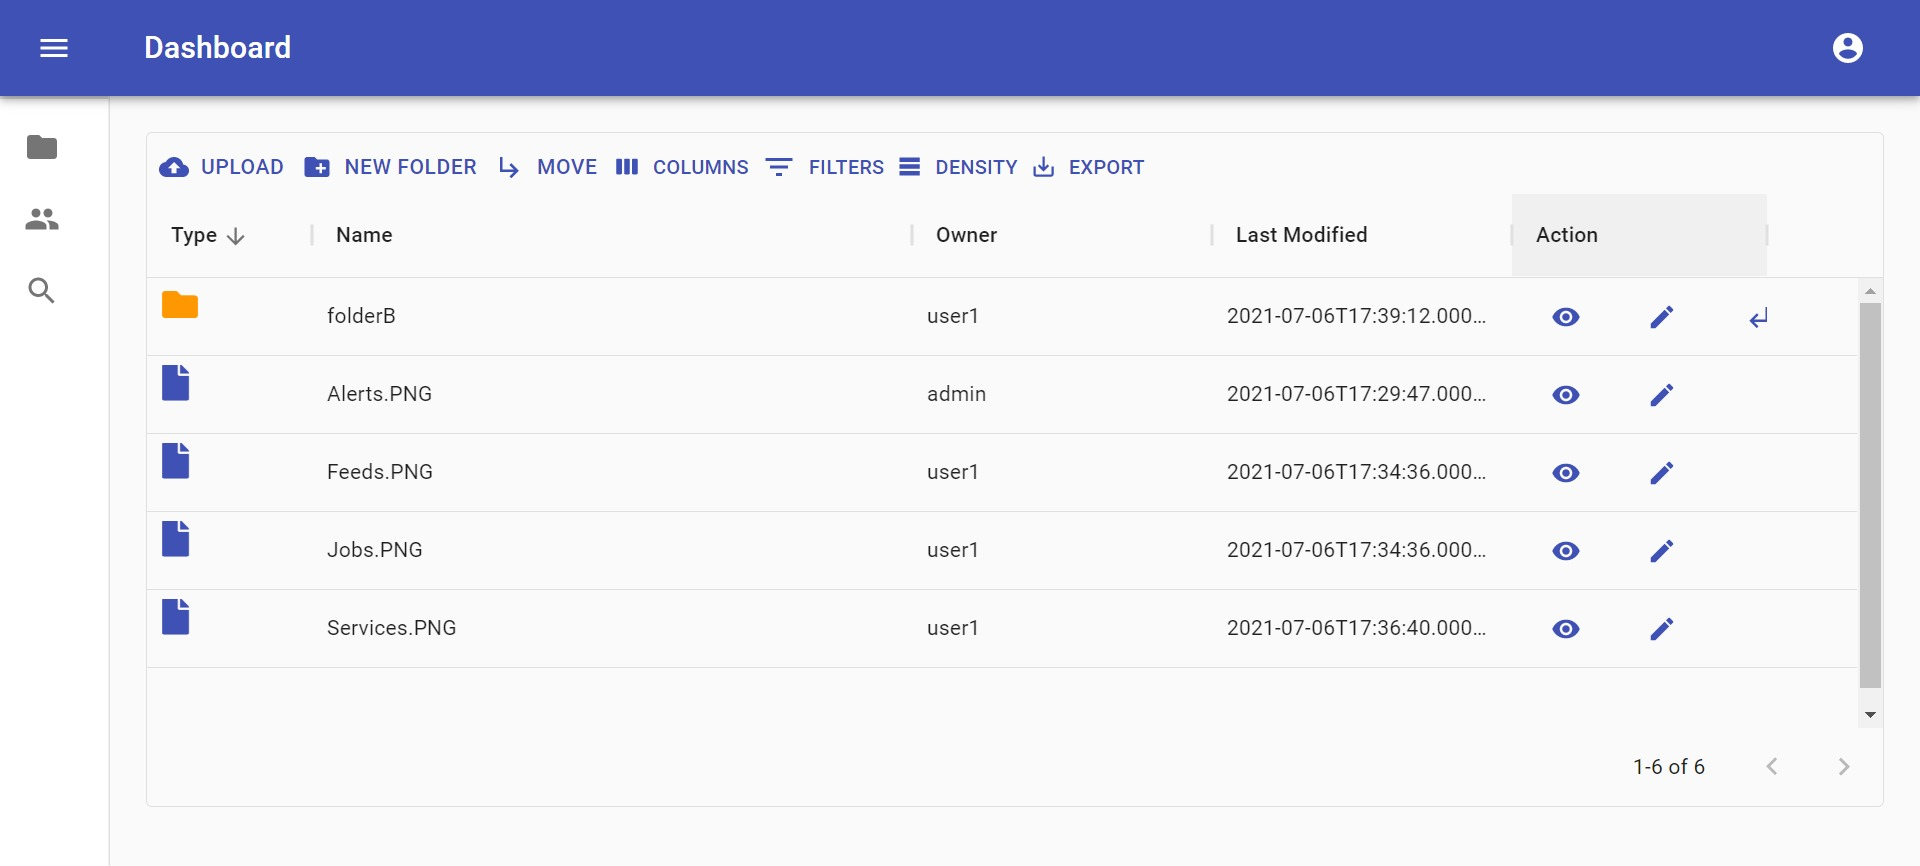
\includegraphics[width=1.0\textwidth]{images/Directory-Listing.jpg}
    \caption{List all files and folders user interface}
    \label{fig:listContent}
\end{figure}
\begin{figure}[H]
    \centering
    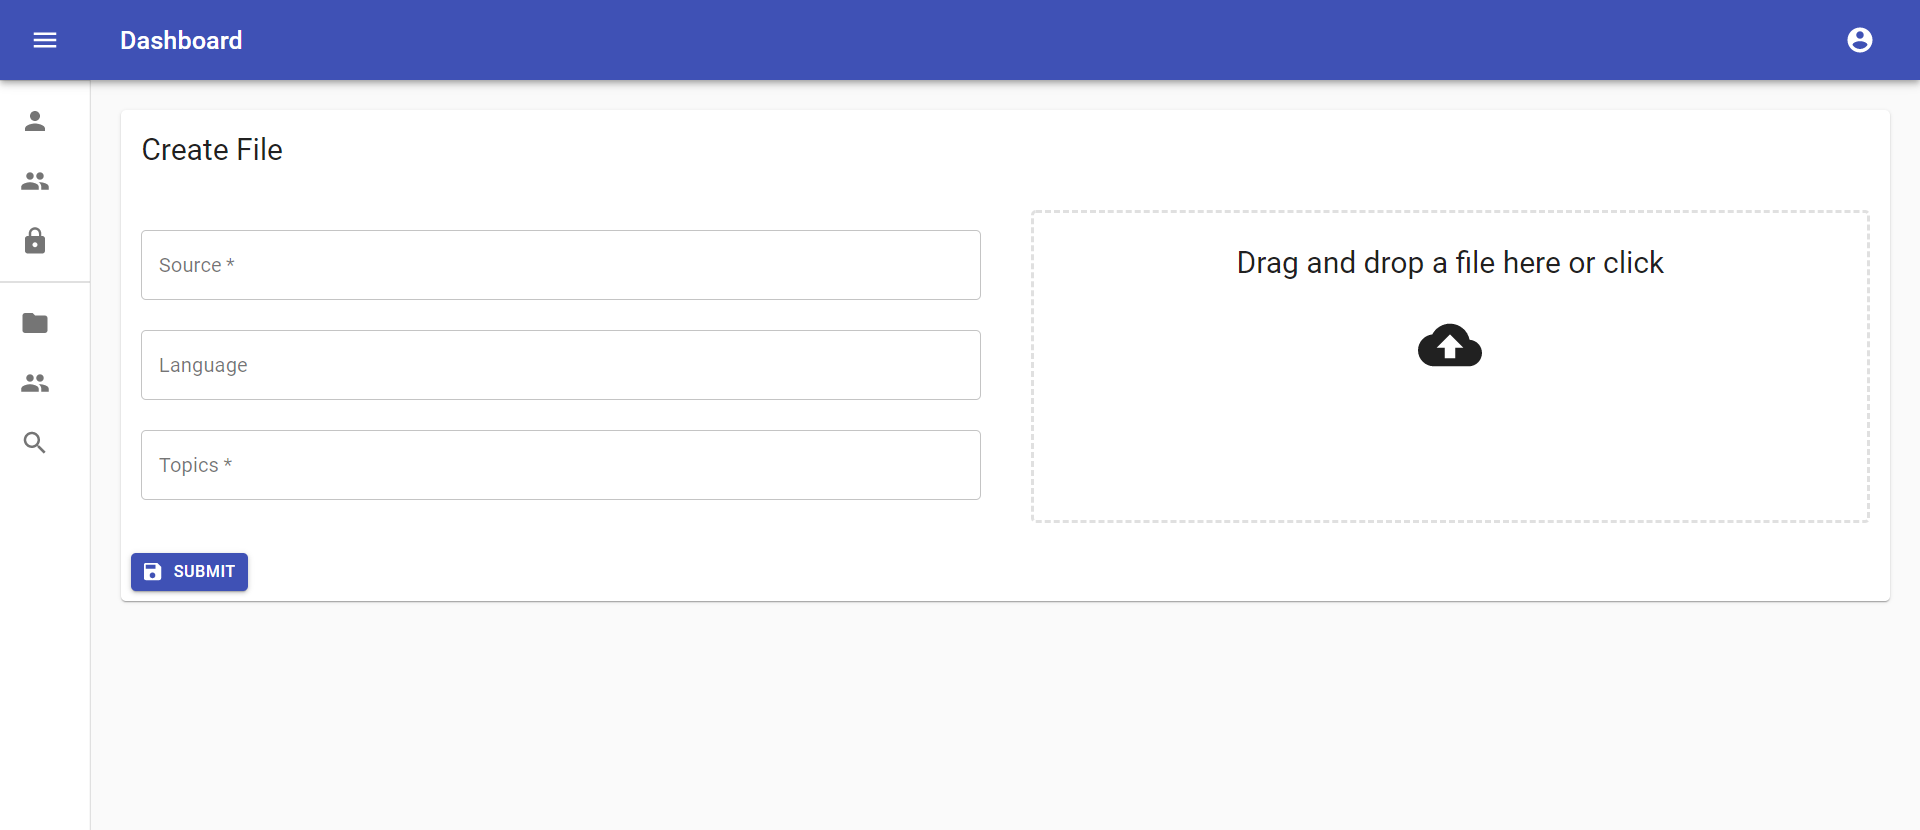
\includegraphics[width=1.0\textwidth]{images/File-Upload.png}
    \caption{Upload File user interface}
    \label{fig:uploadFile}
\end{figure}
\begin{figure}[H]
    \centering
    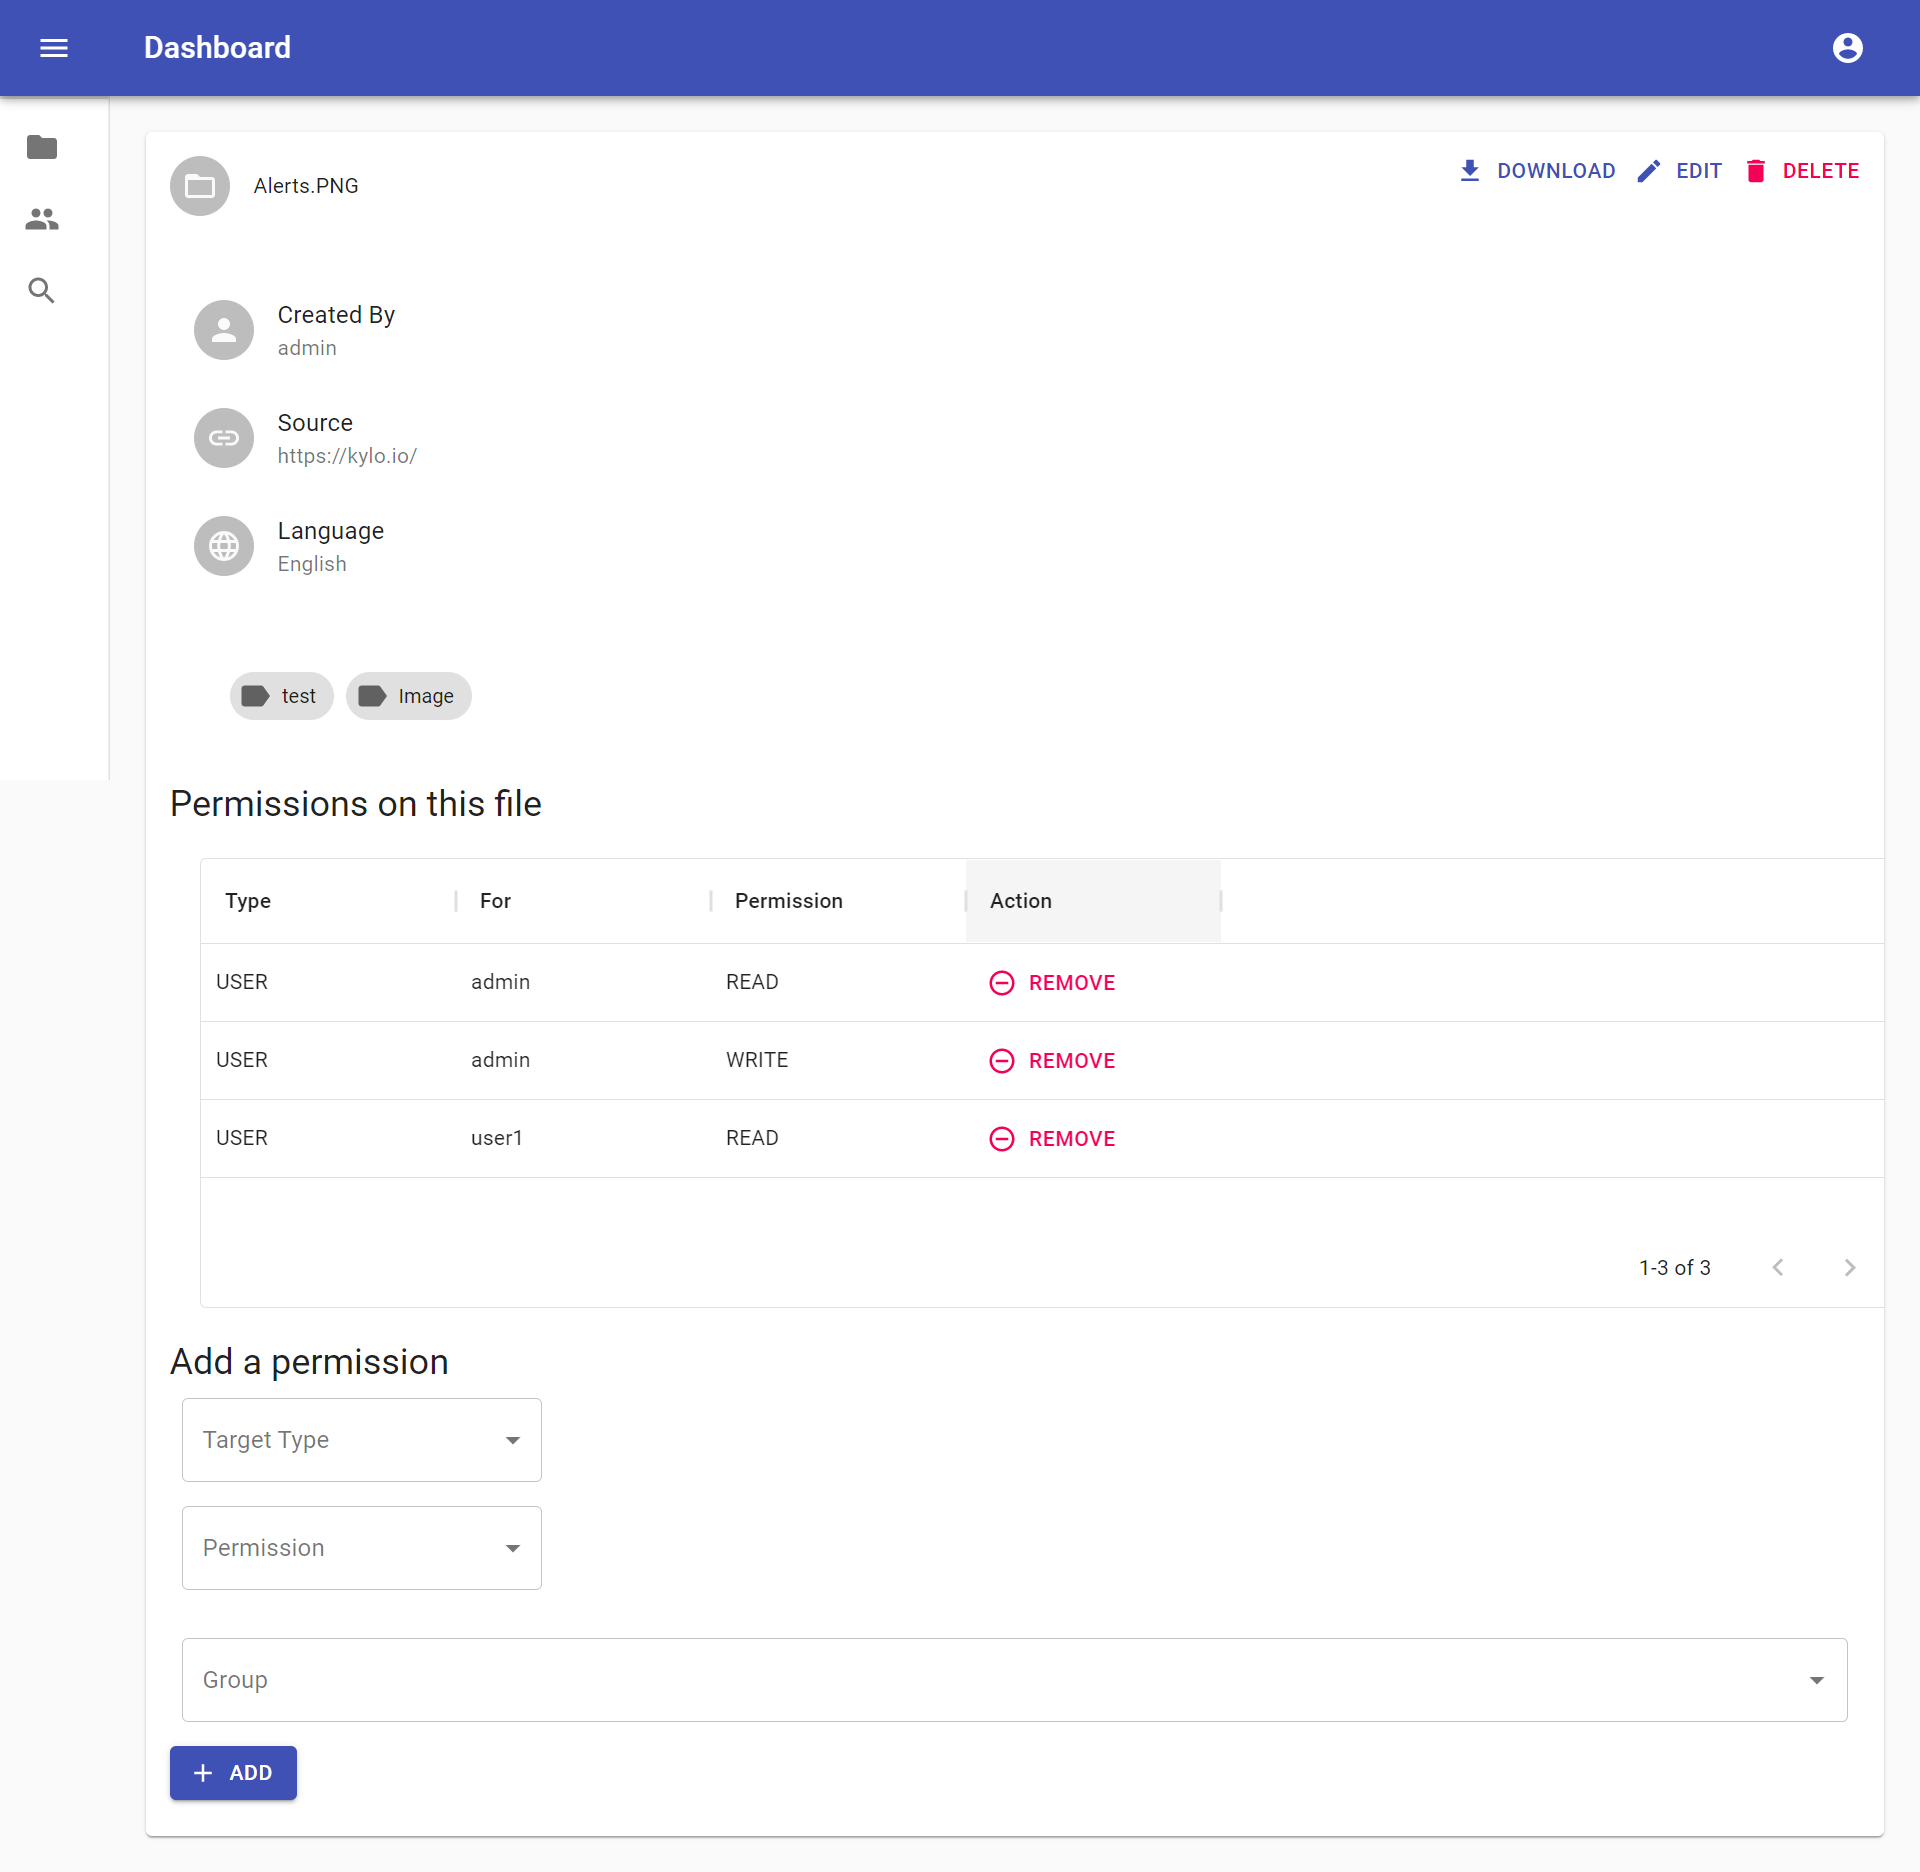
\includegraphics[width=1.0\textwidth]{images/File-ViewDetails.png}
    \caption{View File Details user interface}
    \label{fig:viewFile}
\end{figure}
\begin{figure}[H]
    \centering
    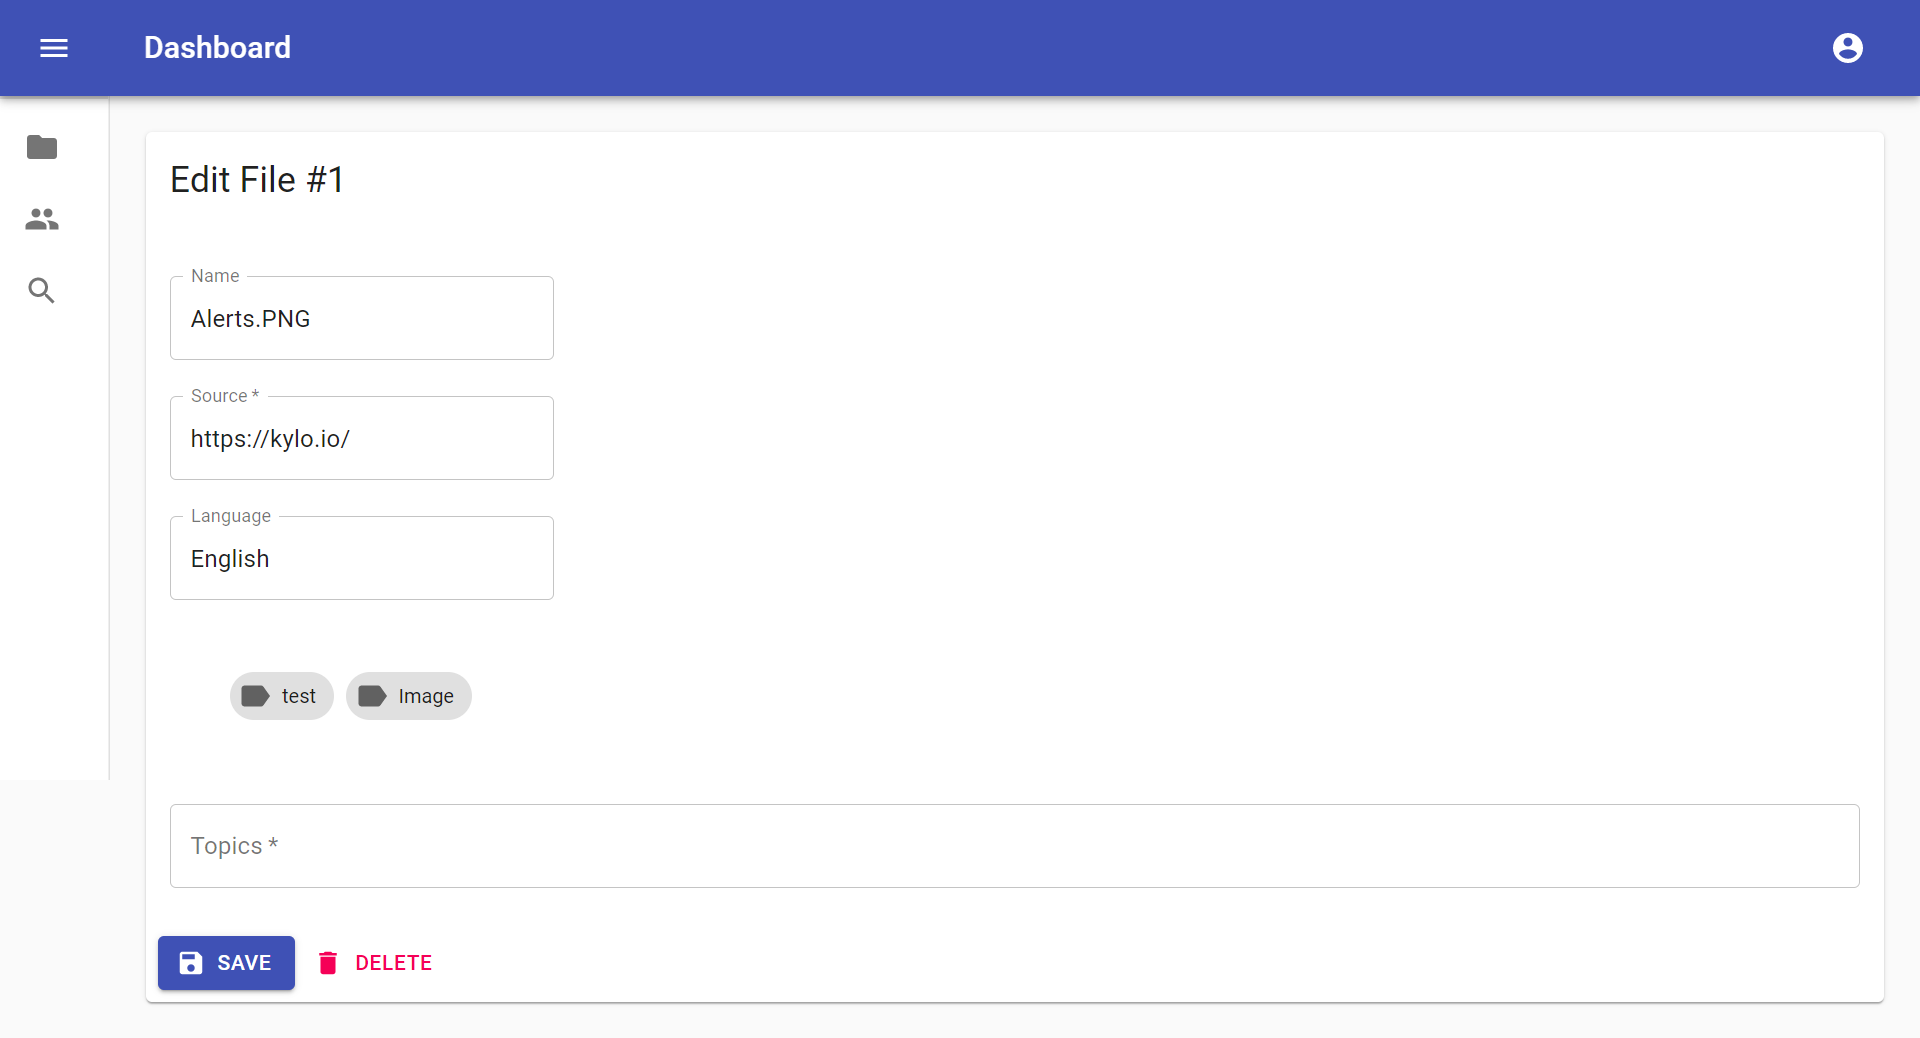
\includegraphics[width=1.0\textwidth]{images/File-Edit.png}
    \caption{Edit File user interface}
    \label{fig:editFile}
\end{figure}
\section{Discussion}
Despite being implemented completely, the main functions in this project have some existing
problems. 

The concept of Data Lake is new to us. And it takes a long time to get a sense of what it is and how to do.

Furthermore, because this website was not created by a team of experienced creators but by a novice individual, it contains numerous flaws in terms of design and features.

Finally, time constraints prevent the testing process from being completed completely and methodically, potentially resulting in a large number of minor problems. On the other hand, this website has accomplished all of the initial objectives listed in the Objectives chapter.

%\chapter{Discussion}
%\label{chap:results}
%\input{chapters/discussion.tex}

\chapter{Conclusions}
\label{chap:conclusions}
\section{Conclusion}
In conclusion, the purposes and objectives of the APIs and Dashboard for Data Lake are achieved. By providing a user-friendly interface on the web, managing data becomes more accessible and more effective.

The main functions have already been implemented:
\begin{itemize}
    \item User can register and log in the system. 
    \item Admin can manage users and user groups. 
    \item User can upload, update and remove any files and folders.
    \item User can grant or remove permission to file or folders they own. 
\end{itemize}
\section{Future Works}
To further improve this web application in the future, the following tasks need to be done: 
\begin{itemize}
    \item Improve web security.
    \item Forgot password. 
    \item Account verification by email.
    \item Scale better when upload and download files.
    \item Upload Folder. 
    \item Create a Guideline for using the system. 
    \item Improve the performance of the application to be more responsive and user-friendly.
\end{itemize}


%%%%%%% Bibliography %%%%%%%%
\printglossary
\printglossary[type=\acronymtype]
\glsaddallunused

\bibliographystyle{bst/IEEEtran} 
\bibliography{bib/IEEEreferences} 
% \addbibresource{references.bib}
% \printbibliography

%%%%%%% Bibliography %%%%%%%%    

\appendix  
\clearpage % o \cleardoublepage
\addappheadtotoc 
\appendixpage 
\stoplist[main]{lof}% stops main list of figures
\startlist[appendix]{lof}% starts list of figures in appendices
\printlist[appendix]{lof}{}{\chapter*{List of Figures in Appendices}}% prints list of figures in appendices
\clearpage
\begin{figure}[H]
    \centering
    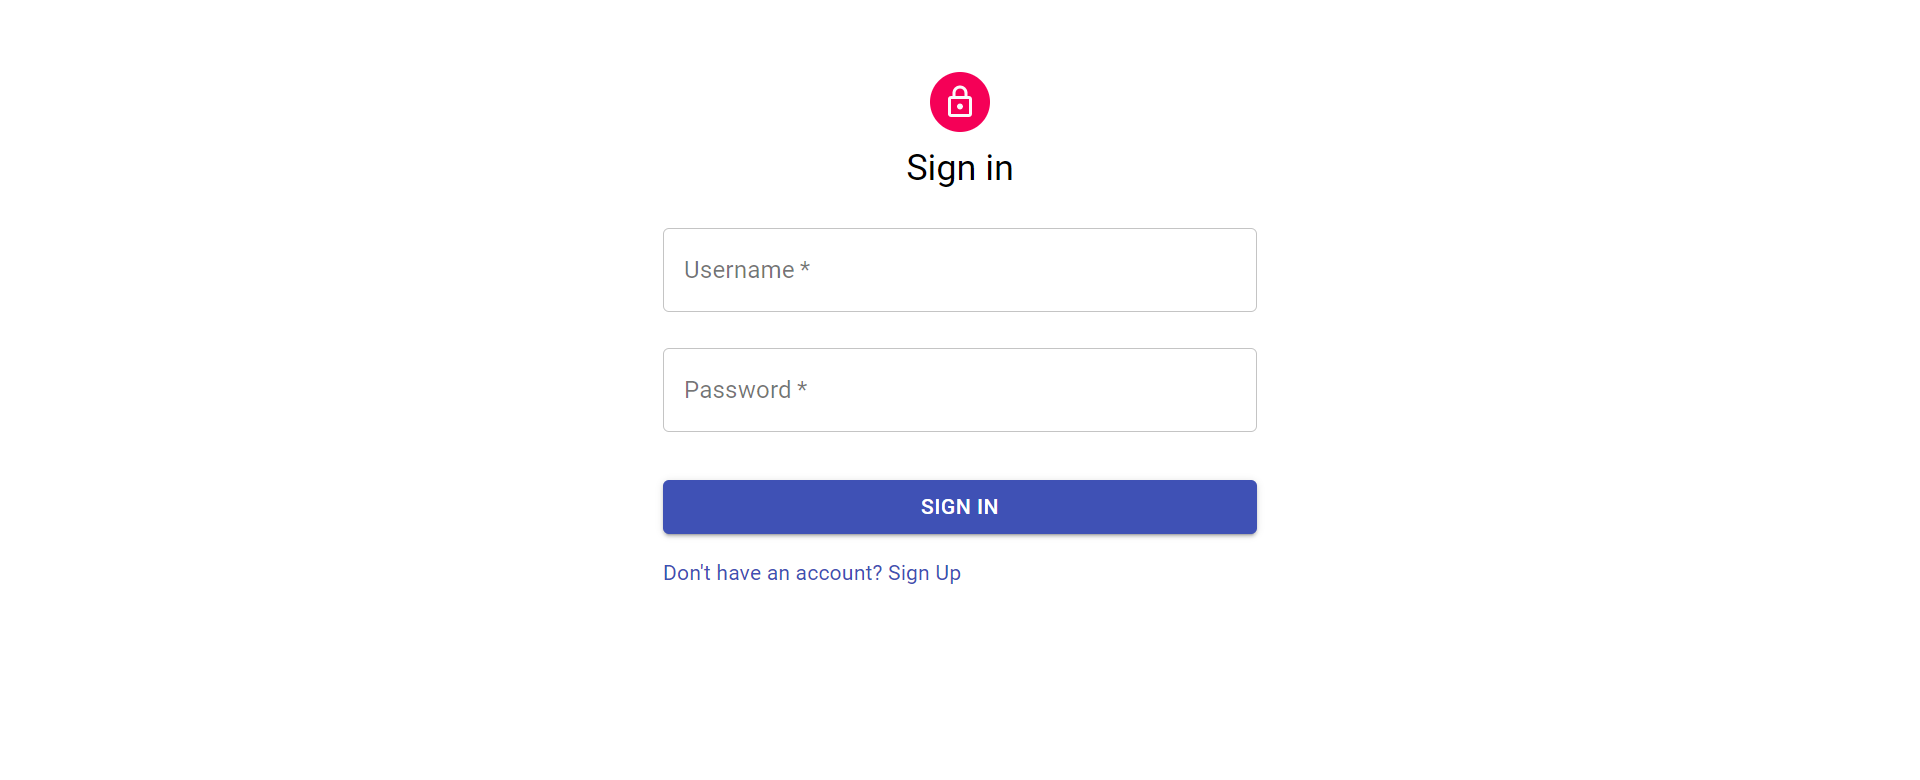
\includegraphics[width=1.0\textwidth]{images/SignIn.png}
    \caption{Login user interface}
    \label{fig:login}
\end{figure}
\begin{figure}[H]
    \centering
    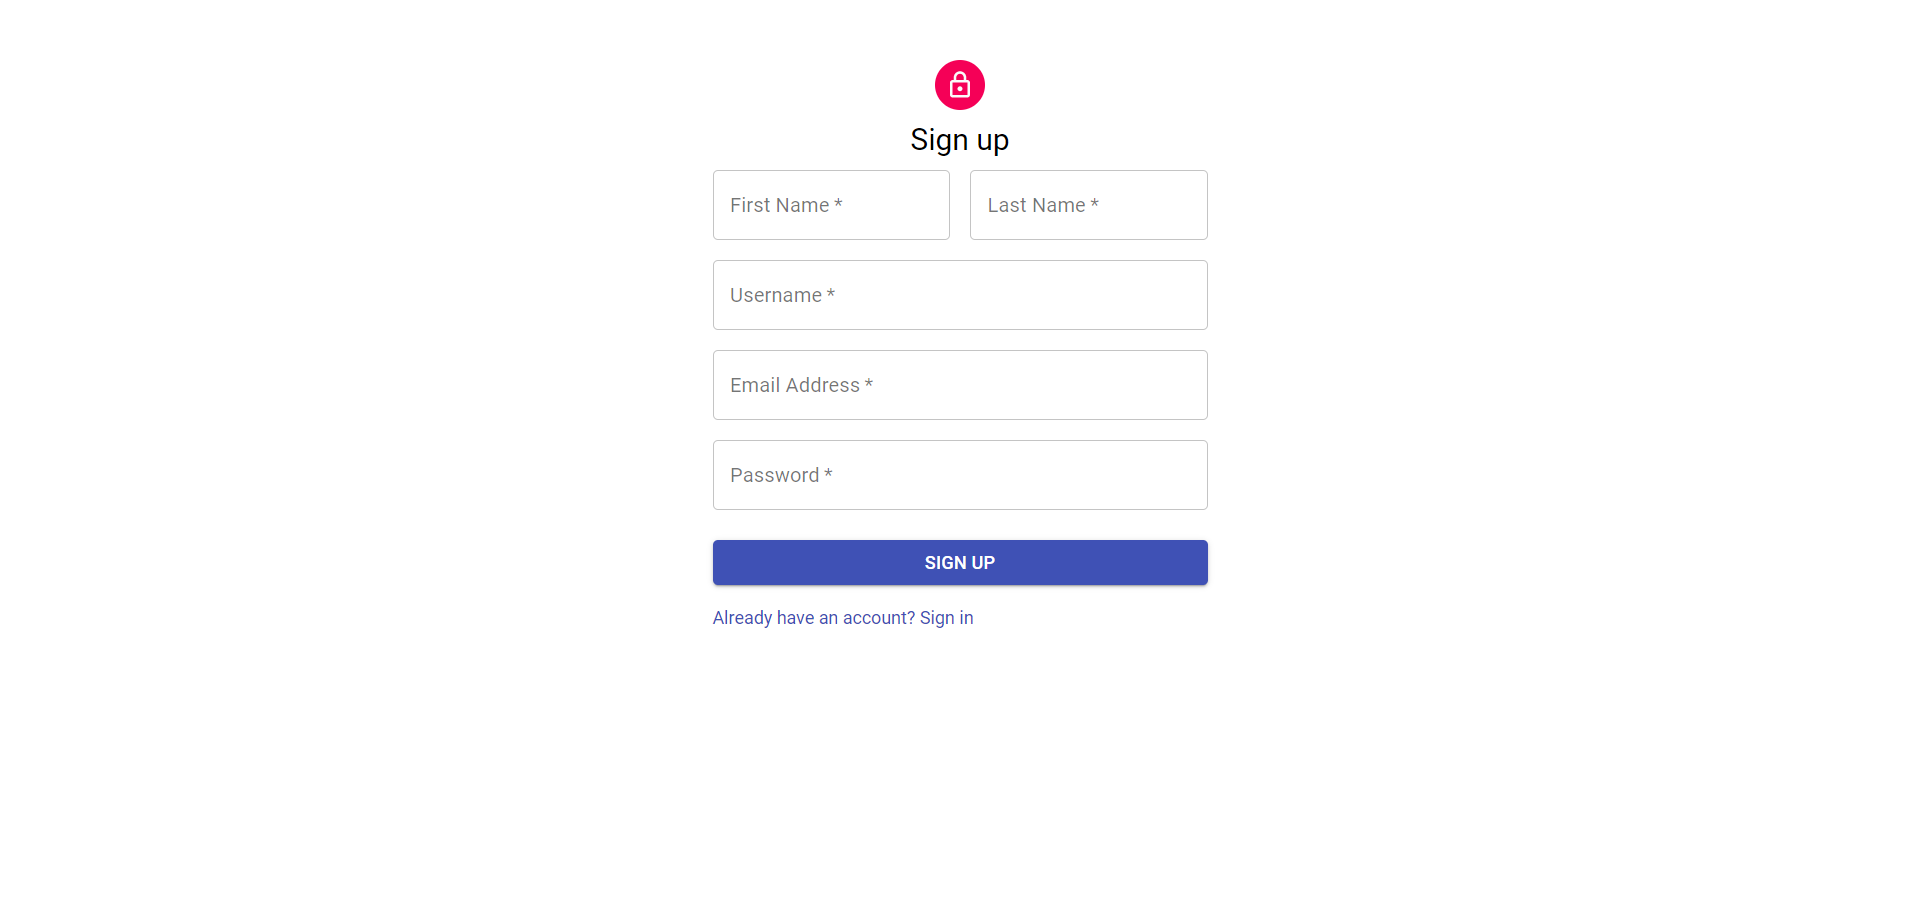
\includegraphics[width=1.0\textwidth]{images/Register.png}
    \caption{Register user interface}
    \label{fig:register}
\end{figure}
\begin{figure}[H]
    \centering
    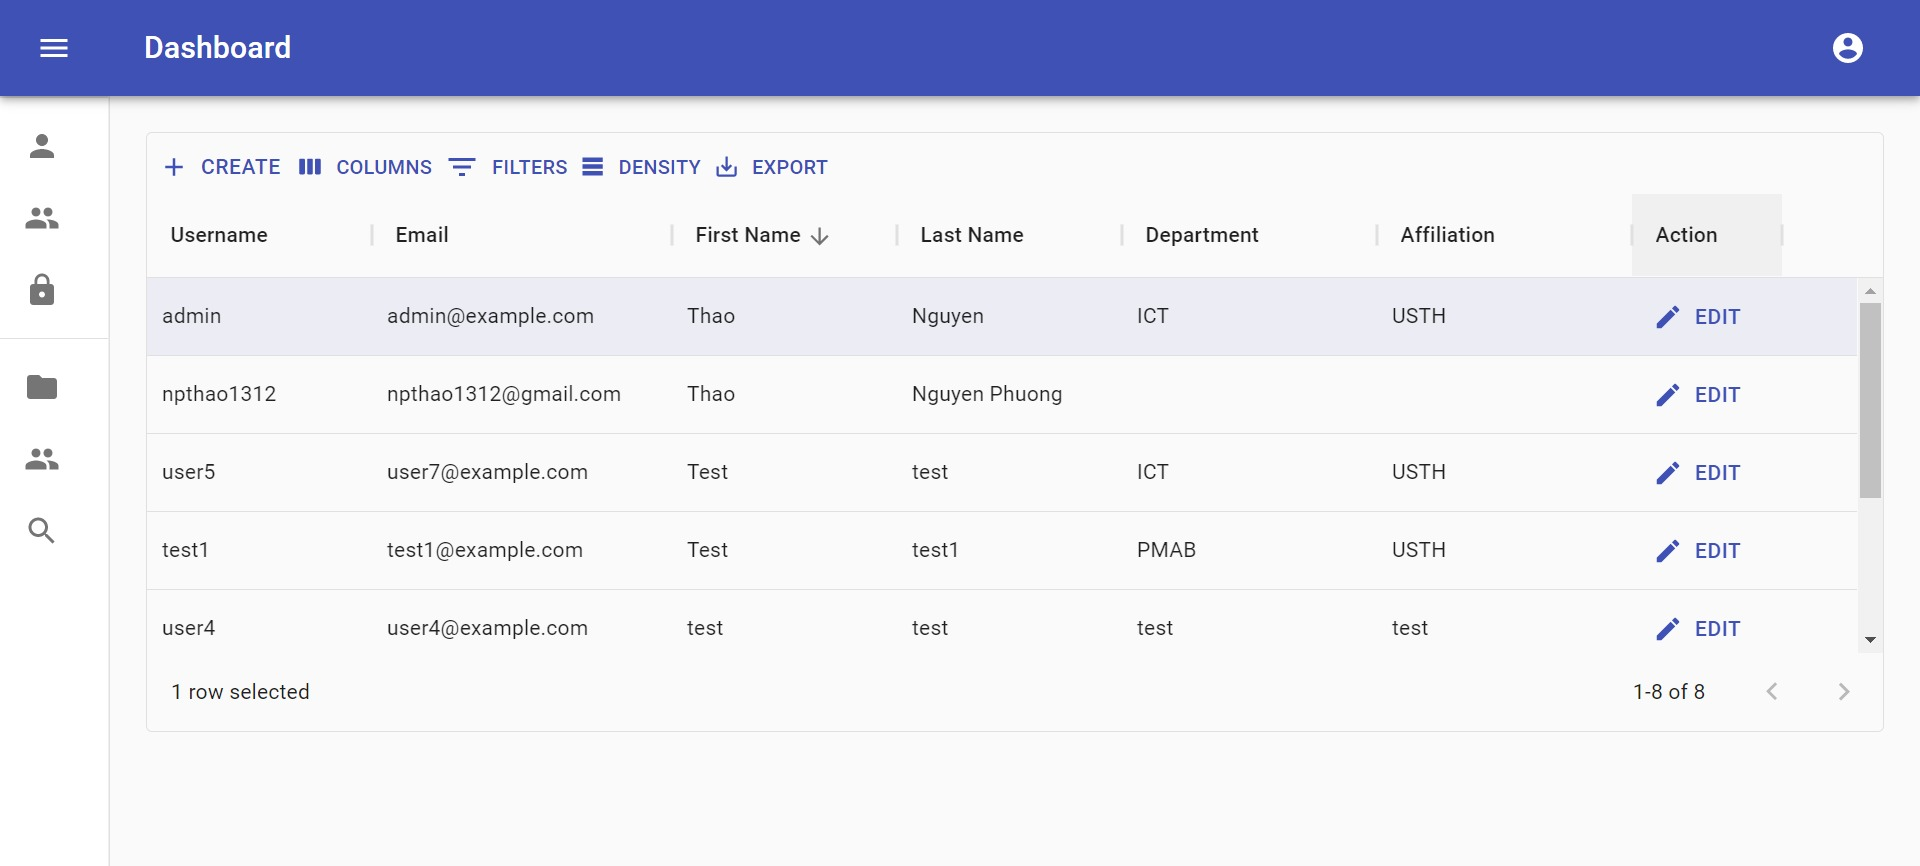
\includegraphics[width=1.0\textwidth]{images/Admin-All-Users.jpg}
    \caption{Admin List All Users user interface}
    \label{fig:adminAllUsers}
\end{figure}
\begin{figure}[H]
    \centering
    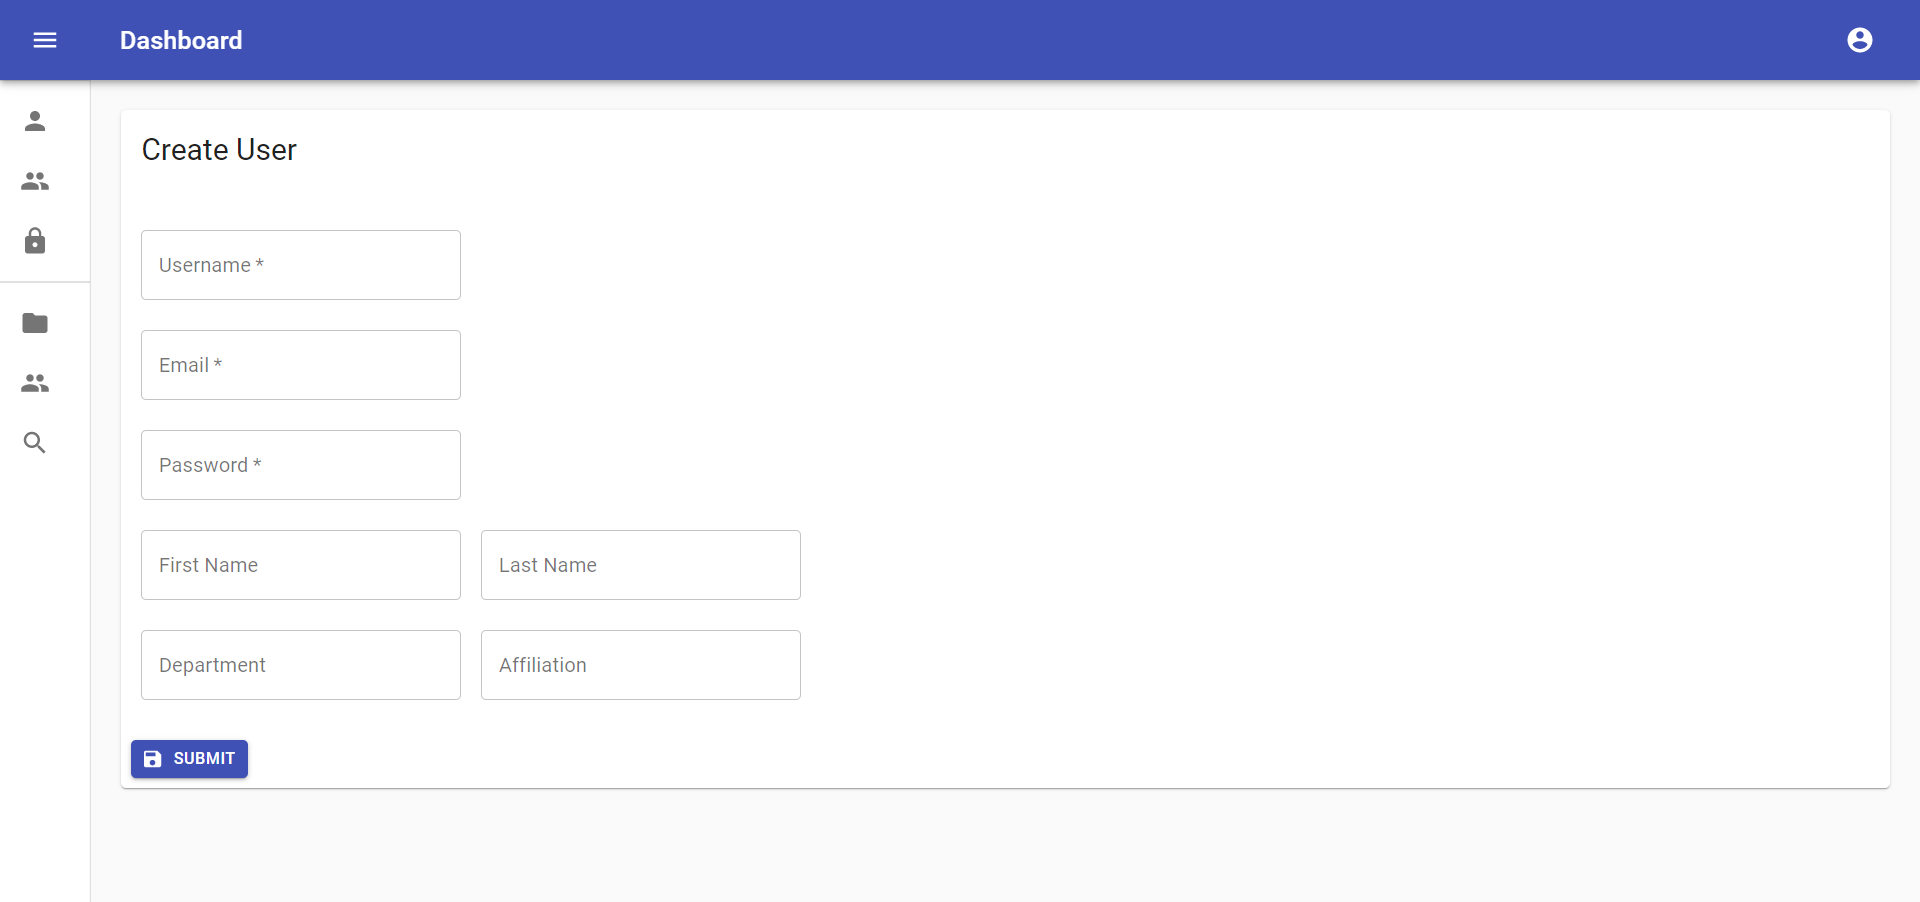
\includegraphics[width=1.0\textwidth]{images/Admin-Create-User.png}
    \caption{Admin Create User user interface}
    \label{fig:adminCreateUser}
\end{figure}
\begin{figure}[H]
    \centering
    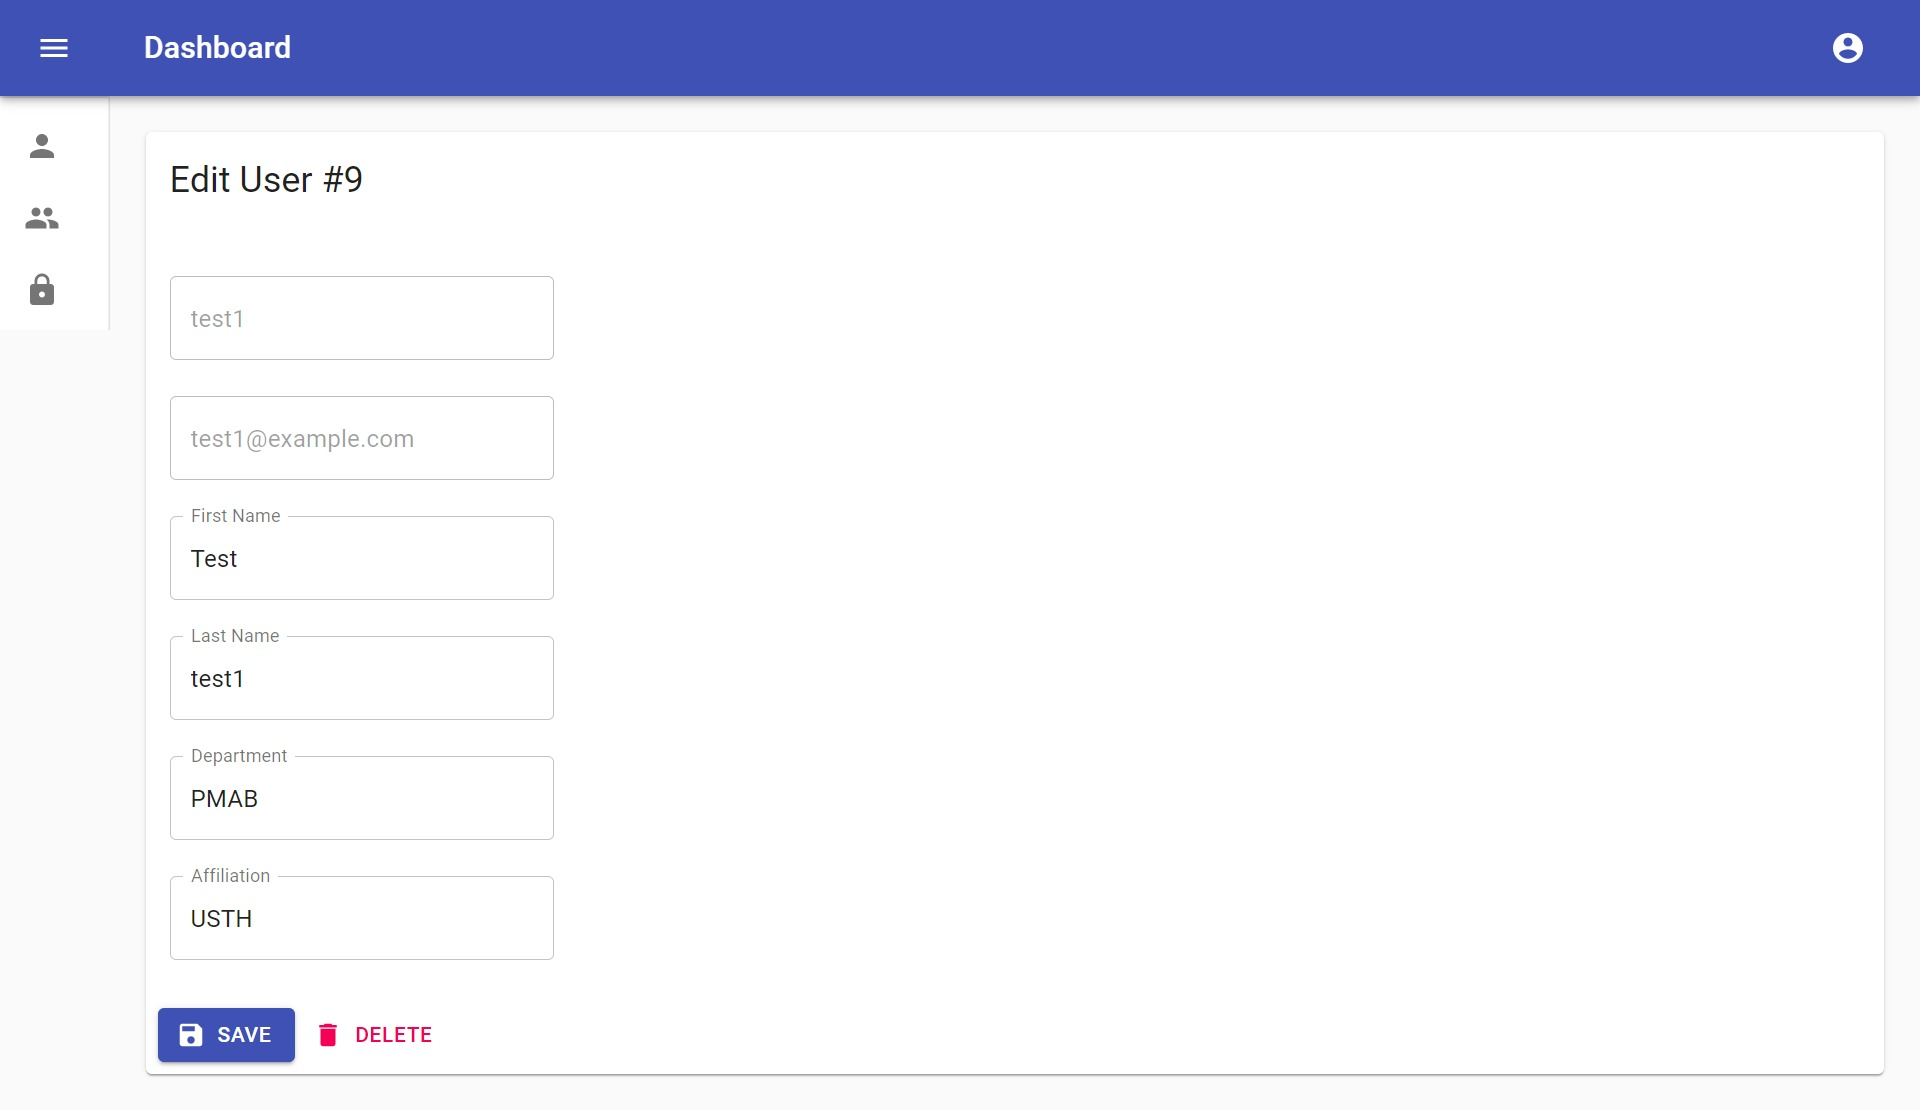
\includegraphics[width=1.0\textwidth]{images/Admin-Edit-User.jpg}
    \caption{Admin Edit and Delete a User user interface}
    \label{fig:adminEditDeleteUser}
\end{figure}
\begin{figure}[H]
    \centering
    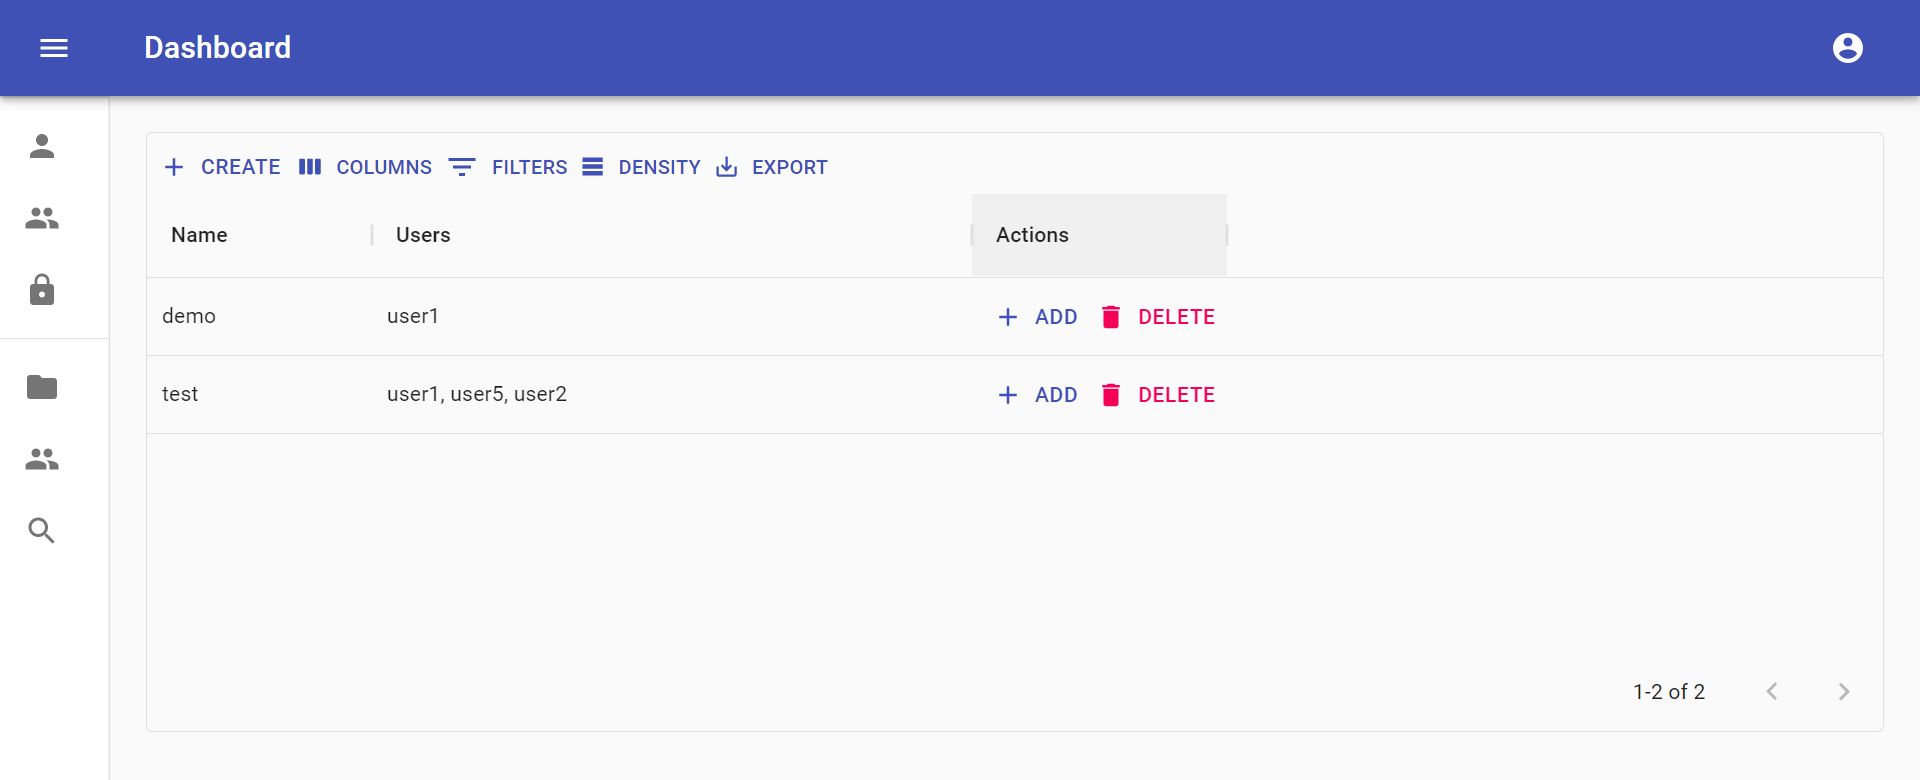
\includegraphics[width=1.0\textwidth]{images/Group-List-Admin.png}
    \caption{Admin List all Groups user interface}
    \label{fig:adminListAllGroups}
\end{figure}
\begin{figure}[H]
    \centering
    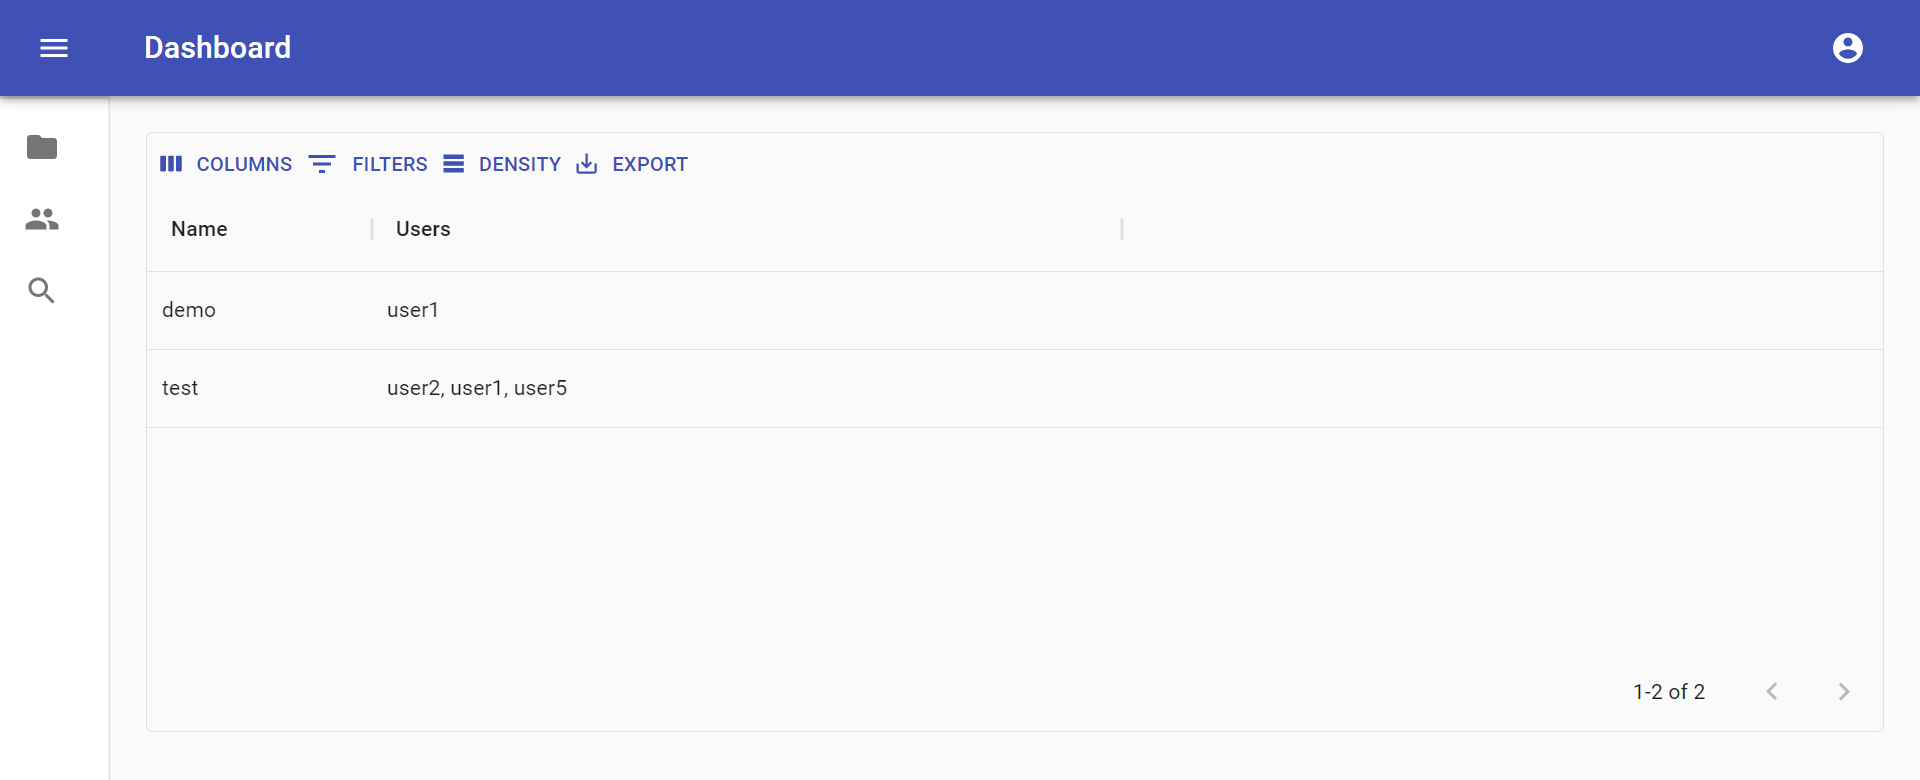
\includegraphics[width=1.0\textwidth]{images/Group-List-Limited-For-User.png}
    \caption{User Limited View List all Groups user interface}
    \label{fig:userListAllGroups}
\end{figure}
\begin{figure}[H]
    \centering
    \includegraphics[width=1.0\textwidth]{images/Group-Create.png}
    \caption{Admin Create Group user interface}
    \label{fig:adminCreateGroup}
\end{figure}
\begin{figure}[H]
    \centering
    \includegraphics[width=1.0\textwidth]{images/Group-Add-User.png}
    \caption{Admin Update Group user interface}
    \label{fig:adminUpdateGroup}
\end{figure}

\begin{figure}[H]
    \centering
    \includegraphics[width=1.0\textwidth]{images/Folder-Create.png}
    \caption{Create Folder user interface}
    \label{fig:createFolder}
\end{figure}
\begin{figure}[H]
    \centering
    \includegraphics[width=1.0\textwidth]{images/Folder-ViewDetails.png}
    \caption{View Folder Details user interface}
    \label{fig:viewFolder}
\end{figure}
\begin{figure}[H]
    \centering
    \includegraphics[width=1.0\textwidth]{images/Folder-Edit.jpg}
    \caption{Edit Folder user interface}
    \label{fig:editFolder}
\end{figure}
\begin{figure}[H]
    \centering
    \includegraphics[width=1.0\textwidth]{images/Move.png}
    \caption{Move File or Folder user interface}
    \label{fig:moveContent}
\end{figure}
\begin{figure}[H]
    \centering
    \includegraphics[width=1.0\textwidth]{images/Update-Profile.png}
    \caption{Update Profile user interface}
    \label{fig:updateProfile}
\end{figure}
\begin{figure}[H]
    \centering
    \includegraphics[width=1.0\textwidth]{images/Search-Dataset.png}
    \caption{Search ACL sources user interface}
    \label{fig:searchContent}
\end{figure}
\begin{figure}[H]
    \centering
    \includegraphics[width=1.0\textwidth]{images/Admin-Acl-List-All.jpg}
    \caption{Admin List all ACLs user interface}
    \label{fig:AdminListAllACLs}
\end{figure}
\begin{figure}[H]
    \centering
    \includegraphics[width=1.0\textwidth]{images/Admin-Grant-Permission.png}
    \caption{Admin Grant a ACL user interface}
    \label{fig:AdminGrantACL}
\end{figure}





\end{document}